\documentclass[12pt]{article}
\usepackage{hyperref}
\usepackage{amsmath}
%\usepackage{amsmath}
\usepackage{graphicx}
\usepackage{xspace}
% \usepackage[extendedchars]{grffile}
\usepackage{chngpage}
\usepackage{calc}
\usepackage{topcapt}
\usepackage{subfig}
\newcommand{\unit}[1]{\ensuremath{\text{\,#1}}\xspace}
\newcommand{\fbinv} {\mbox{\ensuremath{\,\text{fb}^{-1}}}\xspace}
\newcommand{\pbinv} {\mbox{\ensuremath{\,\text{pb}^{-1}}}\xspace}
\newcommand{\npe} {\mbox{\ensuremath{\textrm{N}_\textrm{PE}}\xspace}}


\title{Analysis of the milliQan demonstrator data at the LHC}

\author{M. Citron}

\begin{document}
\maketitle

\section{Introduction}

The collection, calibration and analysis of the milliqan demonstrator data is described below.
The major remaining tasks are:
\begin{itemize}
    \item Rerun excluding bad runs 1350-1380
    \item Make time dependent dark rate estimate (ideally using physics runs)
    \item Add cosmic shower section
    \item Add after pulse section
    \item Add radiation section
    \item Refine signal selection based on simulation for background and signal
    \item \npe dependent signal selection to target higher and lower charges
\end{itemize}

\section{The milliQan demonstrator}

The milliQan demonstrator is positioned in the PX56 drainage gallery in
the site envisioned for the full milliQan detector. PX56 has a diameter of $\sim 2.7$~m. 
With the aid of a 3D model constructed from a laser scan of the tunnel, 
an optimized location has been determined to place milliQan 
that intercepts maximal mCP flux given the constraint that, at the 
chosen angle to the IP, it must be able accommodate the length of the detector. 
The chosen location is almost directly above CMS with a distance to the IP of 
33\unit{m} (17\unit{m} of which is through rock), and at an azimuthal angle of 
43.1 degrees from the horizontal plane. The 3D model showing the location 
of the demonstrator is shown in Fig.~\ref{fig:site}.

The milliQan demonstrator is shown in Figure~\ref{fig:demo}. It
consists of eighteen $5\times5\times80\unit{cm}$ scintillator bars arranged in three layers of 
$2\times3$ scintillator+PMT units. In addition to the bars, ``slabs" of $2.5 \times 20 \times 30\unit{cm}$ 
scintillator and thin panels of $1 \times 18 \times 100\unit{cm}$ scintillator are 
inserted to tag charged particles such as muons from the CMS IP, study backgrounds 
from radiation, and to simulate the active veto of the full detector. There are also 
several hodoscope packs composed of small arrays of $0.75 \times 18$ inch rectangular 
pieces of plastic scintillator readout via SiPMs attached at one end. These provide 
finer grained position information that allows crude tracking through the device. 

\begin{figure}
    \centering
    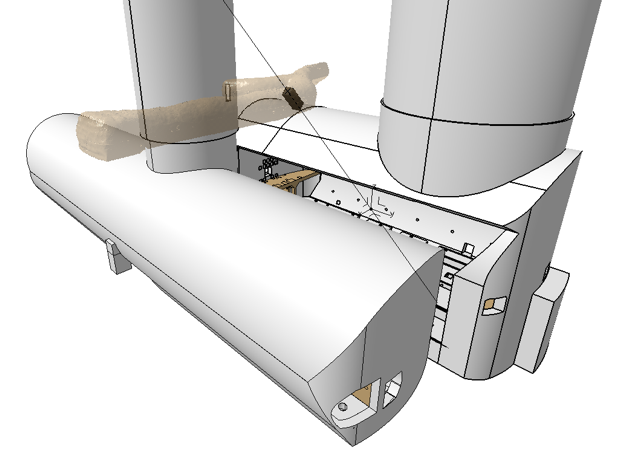
\includegraphics[width=0.6\textwidth]{figures/site_selection_image.png}
  \caption{3D model showing optimal position of milliQan within the PX56 Drainage and Observation gallery located above CMS UXC.\label{fig:site}}
\end{figure}

The demonstrator is held in place using a support structure 
that is able to rotate the demonstrator components into a position
aligned towards the CMS IP. The structure is constructed from a
steel frame that sits on the floor of the tunnel and hosts a 
large bearing allowing the upper part of the structure to rotate 
into alignment. 

The alignment of the demonstrator was performed with the help of the CERN alignment team, 
who installed a set of laser corner cubes that were surveyed into alignment 
with the CMS coordinate system. Laser cubes positioned on the detector are 
aligned by the CERN team with this external coordinate system. The estimated 
accuracy of the procedure is to point the detector to within $10\unit{cm}$ of 
the CMS IP, or about 0.1 degrees, which is more than sufficient for this experiment. 
The alignment is cross-checked using muons from the LHC collisions at the IP using 
the slabs (see Section~\ref{sec:alignment}).

\begin{figure}[bp!]
\centering
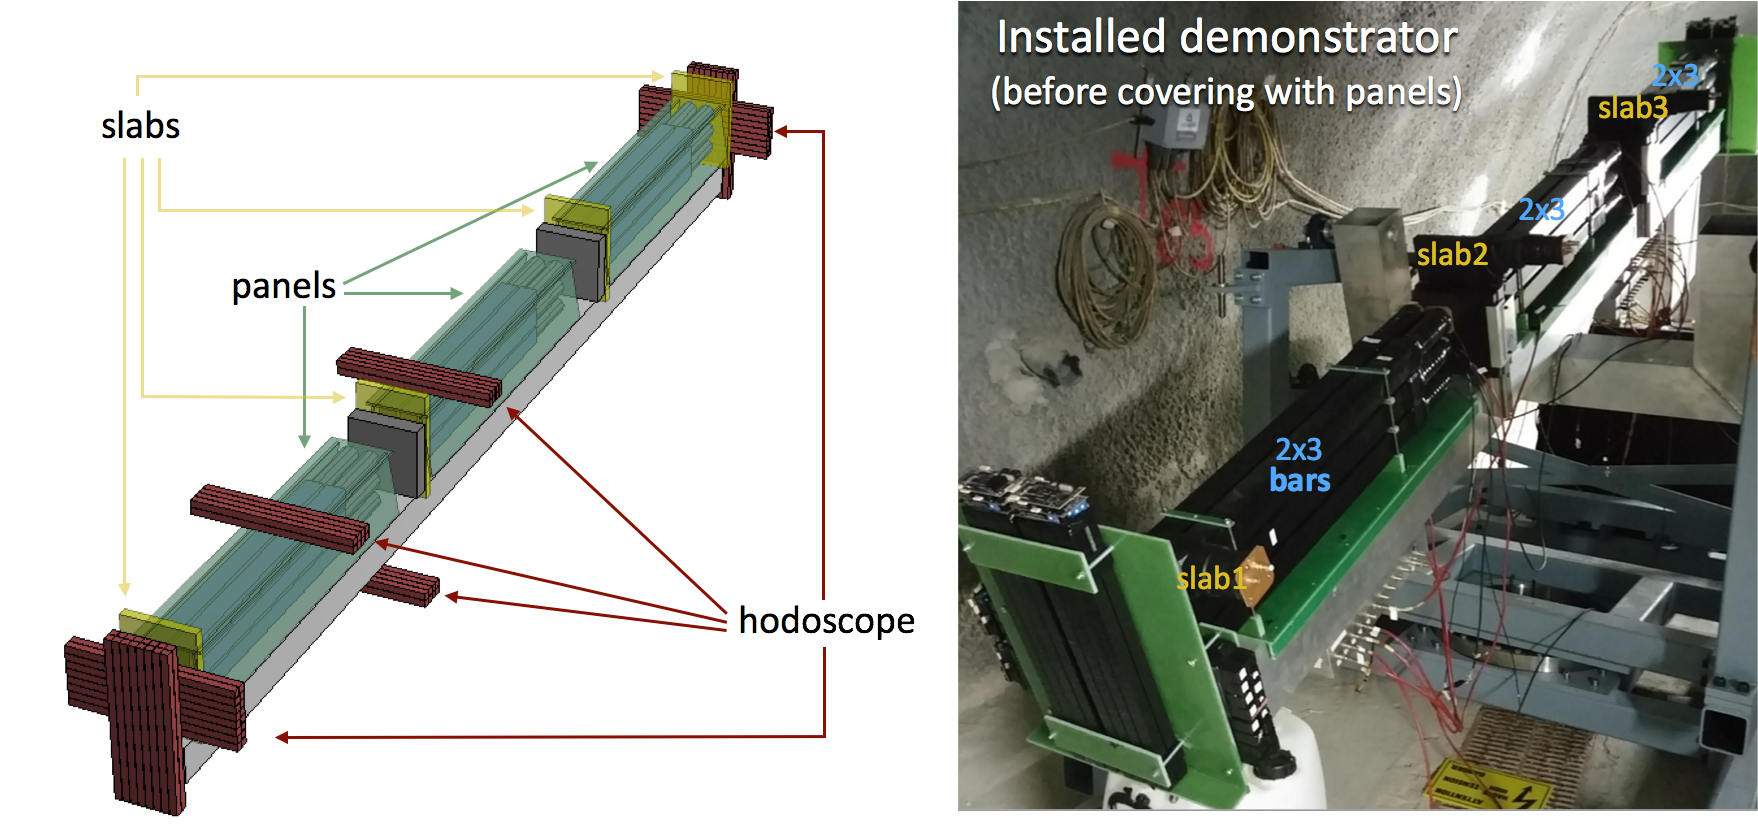
\includegraphics[width=0.89\textwidth]{figures/demonstratorGraphicAndPic}
\caption{Design of the demonstrator and a photo of the demonstrator before covering it with panels.}
\label{fig:demo}
\end{figure}


\begin{figure}
    \centering
    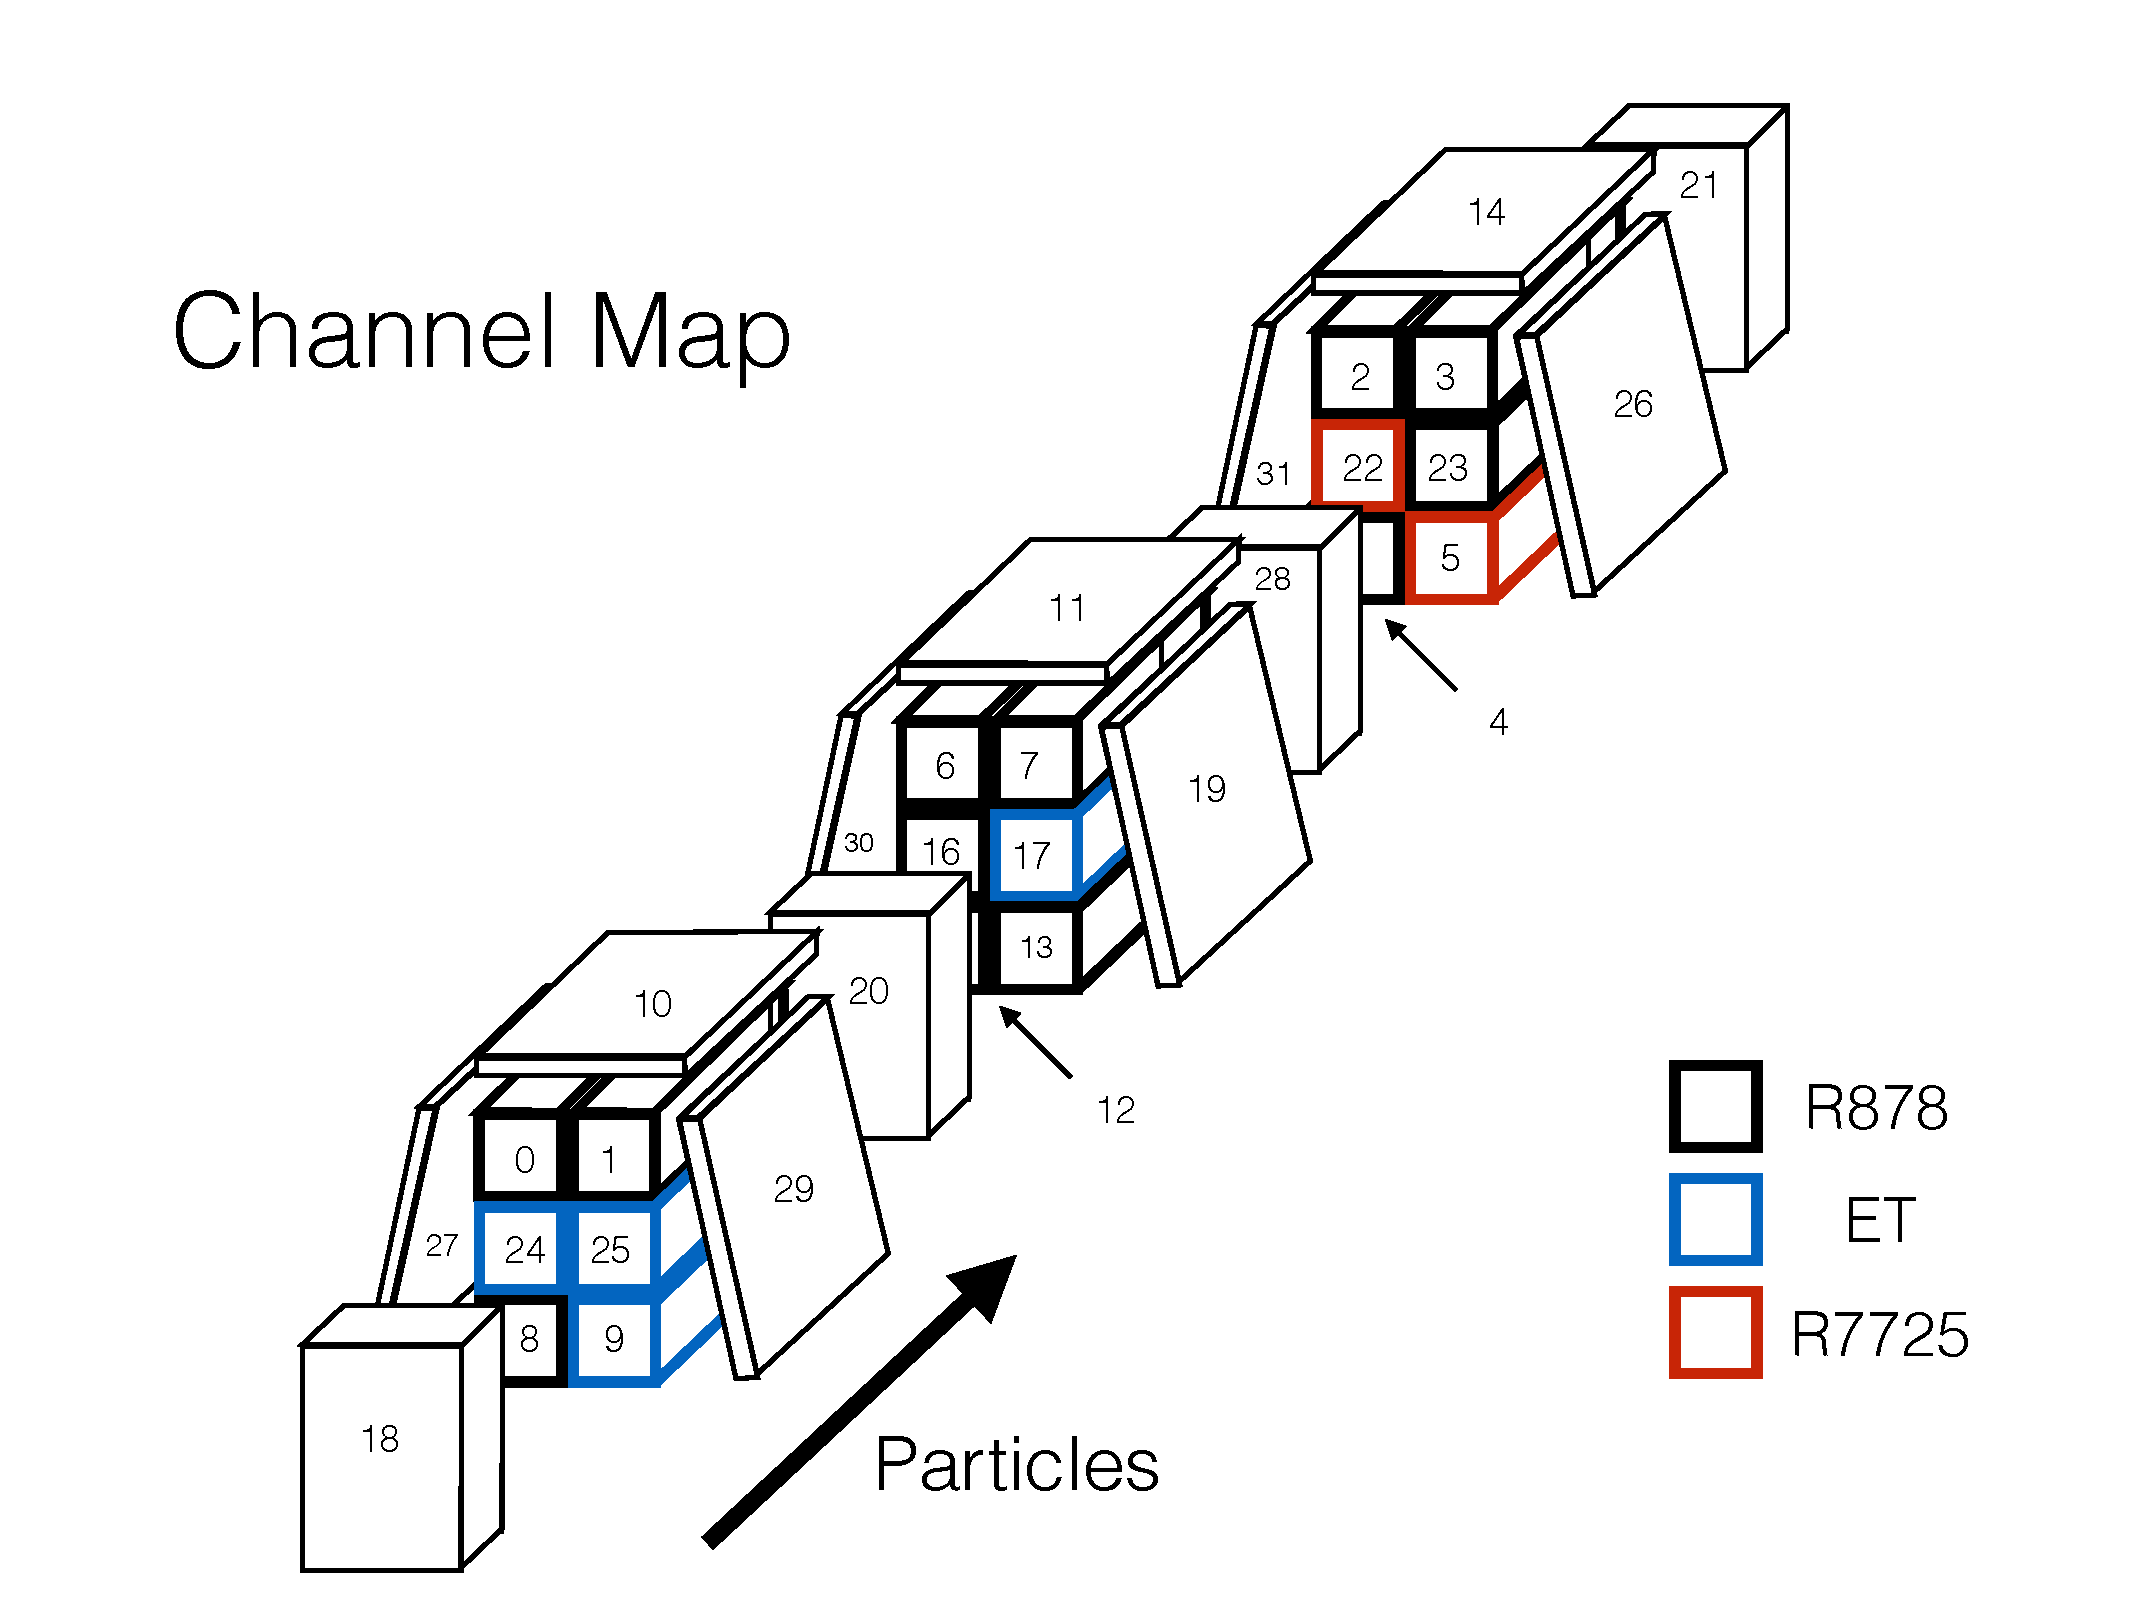
\includegraphics[width=0.6\textwidth]{figures/channelMap}
    \caption{\label{fig:channelMap} The channel mapping for the milliQan demonstrator. 
    The PMT species are indicated by the colour.}
\end{figure}

\section{Data taking}

The data considered in this analysis was collected by the milliQan demonstrator between June 26th 2018 and October 21st 2018.
For all physics quality data, the PMT high voltage is set to $1300\unit{V}$ for the R7725s, $1450\unit{V}$ for the R878s
and $1550\unit{V}$ for the Electron Tubes (ETs). Events are triggered if there is a signal above the trigger threshold 
in three trigger groups within a window of $100\unit{ns}$. Each trigger group contains two channels and the trigger
group for each channel is given by floor(channel/2). The channel mapping ensures adjacent bars are in the same trigger group. 

The trigger thresholds varied during data taking to satisfy rate requirements. The typical 
threshold for the bars ranges from $2.4--7\unit{mV}$, the typical value for the slabs ranges from $150-400\unit{mV}$ and 
for the panels ranges from $2.5--40\unit{mV}$.
%FIXME Add correct values for all years (info needed in tree!)

The total data taking time of all physics runs is $2014.6\unit{h}$. When the data taking rate is high
events may not be properly synchronised between the two digitiser boards used for reading channels 0-15 and 
channels 16-32. To reject unsynchronised events, a requirement is made that both boards record
the TDC time. The efficiency of this selection is $\sim 95\%$ giving an effective total
time of $1906.4\unit{h}$, with approximately $876.9\unit{h}$ and $1029.5\unit{h}$ 
taken during between periods with and without LHC proton-proton collisions respectively.
The total proton-proton luminosity collected is $37.2\fbinv$, of which $35.1\fbinv$ 
satisfies the synchronisation requirement. 

\begin{table}[ht!]
    \scriptsize
    \centering
    \topcaption{
	Mean and RMS for each channel measured in the sideband region of a physics run \label{tab:sideband}
    }
    \begin{tabular}{lll}
	Channel & Sideband mean (mV)& Sideband RMS (mV)\\
	\hline
	    0 & -0.2453  & 0.8637    \\      
	    1 &  0.009&     0.7901   \\
	    2 &  -0.007  &  0.9028   \\ 
	    3 &  -0.07&     0.7561   \\
	    4 &  -0.661&    0.8741   \\
	    5 &  -0.252&    0.7857   \\
	    6 &  0.080&     0.8706   \\
	    7 &  -0.214&    0.7795   \\
	    8 &  -1.04&     0.8098   \\
	    9 &  -0.160&    0.7954   \\
	    10 & 1.18&      0.9941   \\
	    11 & -0.910&    0.7833   \\
	    12 & -0.3789 &  0.9148   \\  
	    13 & -1.09&     0.7899   \\
	    14 & -0.53&     0.9600   \\
	    15 & --&        --       \\
	    16 & -0.367&    0.8829   \\
	    17 & -0.837&    0.8828   \\
	    18 & -0.283&    0.8908   \\
	    19 & -0.275&    0.8005   \\
	    20 & -0.235&    0.8400   \\
	    21 & -0.295&    0.8863   \\
	    22 & -0.443&    1.061    \\
	    23 & -0.606&    0.8085   \\
	    24 & -0.762&    0.9275   \\
	    25 & -0.201&    0.8194   \\
	    26 & -0.576&    0.9087   \\
	    27 & -0.440&    0.7757   \\
	    28 & -0.706&    0.8507   \\
	    29 & -0.426&    0.9169   \\
	    30 & -0.280&    0.9577   \\
	    31 & -0.458  &  0.8018   \\ 
    \end{tabular}
\end{table}
\section{Reconstruction}

The data taken by the demonstrator is comprised of ``waveforms" of voltage against time for each channel.
In order to reconstruct the deposits of particles in the scintillator, ``pulses" are reconstructed from
each waveform. 

With a sampling rate of 1.6 Ghz, the waveforms span $0$ to $650\unit{ns}$ (with the pulse
that causes the trigger to accept the event placed at $\sim360-390 \unit{ns}$ during 
triple coincidence running).
The waveforms may have a significant pedestal which is measured using the mean
value of the amplitude in a sideband region of the waveform from $0-50 \unit{ns}$.
The mean value of this pedestal measurement for each channel in a physics run 
is used to define a pedestal subtraction with the values
shown in Table~\ref{tab:sideband}. Significant drifts are seen in the pedestal for channel 30
and so a subtraction is made using the sideband pedestral measurement per event.

Pulses are reconstructed from the waveforms after the pedestral subtraction.
Starting from the first sample after the sideband region, the 
algorithm considers each time sample consecutively and runs as 
follows until a pulse is started:

\begin{itemize}
    \item If the sample is above the start threshold in Table~\ref{tab:pulseFinding}, increment the pulse starting counter.
    \item If the sample is below the reset threshold in Table~\ref{tab:pulseFinding}, reset the pulse starting counter. This threshold is set as the start threshold minus half the sideband RMS shown in Table~\ref{tab:sideband}.
    \item If the pulse starting counter reaches the N samples above start threshold value shown in Table~\ref{tab:pulseFinding}, start a pulse.
\end{itemize}

Once a pulse has been started the pulse end is determined by continuing as follows:

\begin{itemize}
    \item If the sample is below the start threshold in Table~\ref{tab:pulseFinding}, increment the pulse ending counter. 
    \item If the sample is above the reset pulse end threshold in Table~\ref{tab:pulseFinding} reset the pulse ending counter. This threshold is set as the start threshold plus half the sideband RMS shown in Table~\ref{tab:sideband}.
    \item if the pulse ending counter reaches the N samples below start threshold value shown in Table~\ref{tab:pulseFinding}, end the pulse.
\end{itemize}

Each pulse has several attributes defined as follows:

\begin{itemize}
    \item time: The time of the last sample below the start threshold before the pulse is started.
    \item calibrated time: The calibrated time of the pulse as defined in Section~\ref{sec:timeCalibration}.
    \item duration: The time of the sample after that which triggers the pulse ending minus the time of the last sample below the start threshold.
    \item height: The maximum amplitude in the pulse.
    \item area: The sum of the amplitudes across the pulse.
    \item \npe: The number of photo-electrons (PEs) defined as the pulse area divided by the single PE (SPE) area for each channel (measured as described in Section~\ref{sec:npeCalibration}).
    \item delay: Time between start of this pulse and end of previous pulse.
\end{itemize}

\begin{table}[ht!]
    \scriptsize
    \centering
    \topcaption{
	Pulse finding thresholds. \label{tab:pulseFinding}
    }
    \begin{tabular}{lllll}
	N samples above & N samples below& Start threshold (mV) & Reset threshold (mV) & End threshold (mV)\\
	start threshold & end threshold &  &  & \\
	\hline
	7 & 13 & 2.0 & 1.57 & 2.43\\
	7 & 13 & 2.0 & 1.60 & 2.40\\
	9 & 13 & 2.3 & 1.85 & 2.75\\
	7 & 13 & 2.0 & 1.62 & 2.38\\
	7 & 13 & 2.2 & 1.76 & 2.64\\
	5 & 4 & 2.0 & 1.61 & 2.39\\
	7 & 13 & 2.0 & 1.56 & 2.44\\
	7 & 13 & 2.0 & 1.61 & 2.39\\
	7 & 13 & 2.0 & 1.60 & 2.40\\
	4 & 4 & 2.0 & 1.60 & 2.40\\
	7 & 13 & 2.2 & 1.70 & 2.70\\
	7 & 13 & 2.0 & 1.61 & 2.39\\
	7 & 13 & 2.0 & 1.54 & 2.46\\
	8 & 13 & 2.0 & 1.61 & 2.39\\
	9 & 13 & 2.3 & 1.82 & 2.78\\
	7 & 13 & 2.5 & 2.00 & 3.00\\
	7 & 13 & 2.0 & 1.56 & 2.44\\
	4 & 4 & 2.0 & 1.56 & 2.44\\
	8 & 13 & 2.0 & 1.55 & 2.45\\
	7 & 13 & 2.0 & 1.60 & 2.40\\
	7 & 13 & 2.0 & 1.58 & 2.42\\
	8 & 13 & 2.0 & 1.56 & 2.44\\
	5 & 4 & 3.7 & 3.17 & 4.23\\
	7 & 13 & 2.0 & 1.60 & 2.40\\
	4 & 4 & 2.0 & 1.54 & 2.46\\
	4 & 4 & 2.0 & 1.59 & 2.41\\
	7 & 13 & 2.0 & 1.55 & 2.45\\
	7 & 13 & 2.0 & 1.61 & 2.39\\
	7 & 13 & 2.0 & 1.57 & 2.43\\
	7 & 13 & 2.0 & 1.54 & 2.46\\
	7 & 13 & 2.0 & 1.52 & 2.48\\
	7 & 13 & 2.0 & 1.60 & 2.40\\
    \end{tabular}
\end{table}

\section{Calibration}

\subsection{Charge response calibration}
\label{sec:npeCalibration}
The calibration of the \npe per unit charge incident on the 
detector is crucial for determining the lowest charge to which milliQan can be sensitive. 
To achieve this, we first compute the number of PEs for cosmic muons 
incident on the demonstrator. The value for \npe is extracted by dividing the pulse area of cosmic 
muons by the pulse area of a single PE obtained from delayed scintillation PEs. The 
method of using delayed scintillation PEs to measure the SPE response was validated using 
an LED bench measurement as described in App.~\ref{app:speLEDCalib}. 
To avoid saturation effects the pulse area of cosmic muons 
was measured at lower PMT voltage and extrapolated to the operating voltage.

\begin{figure}
%\begin{figure}[bp!]
\centering
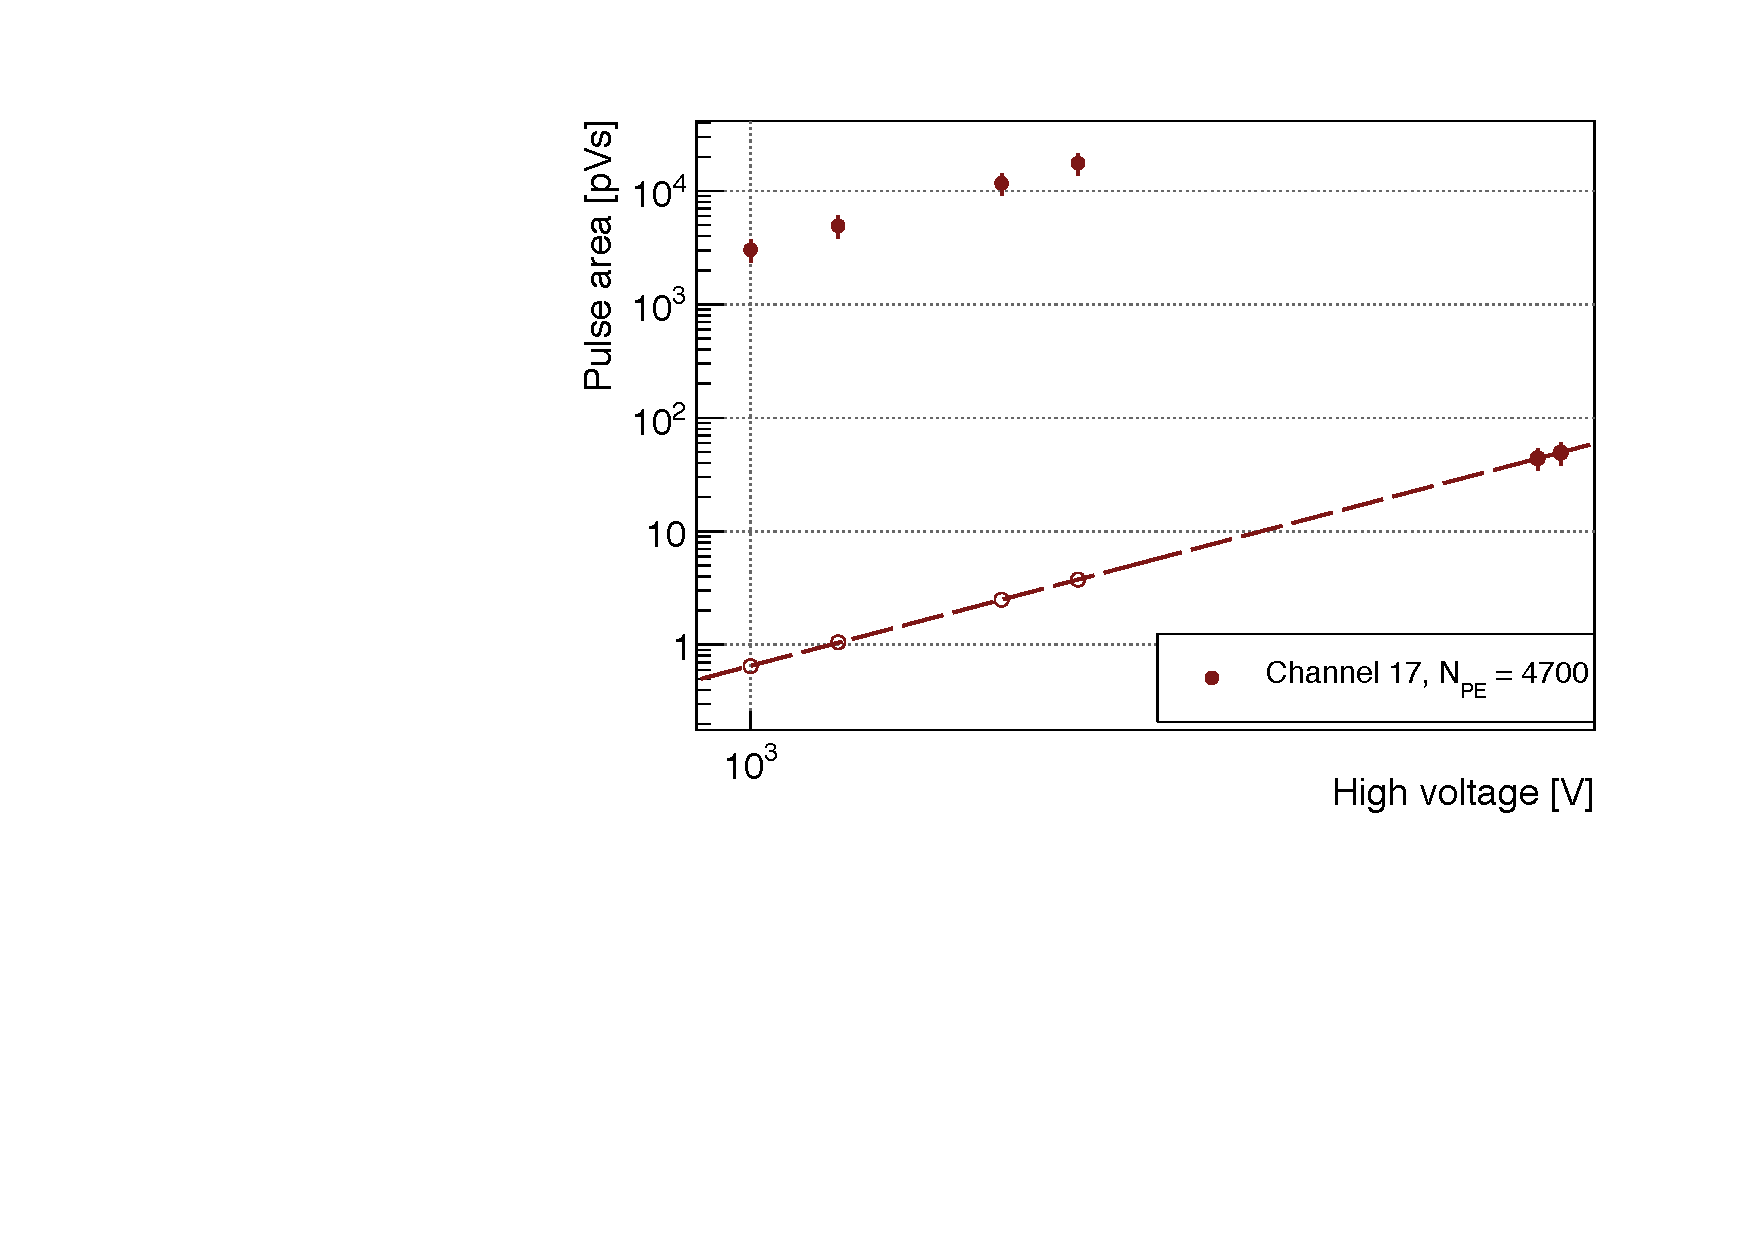
\includegraphics[width=0.6\textwidth]{figures/chargeCalibration.pdf}
\caption{Area versus PMT voltage for a representative PMT for muon and single PEs. A simultaneous fit of the gain curve for the muon and SPE signals, with a floating cosmic photon yield, allows the \npe for $Q=1$ to be determined.}
\label{fig:chargeCalib}
\end{figure}

Figure~\ref{fig:chargeCalib} shows the charge calibration for a representative PMT. The typical value of the 
measured \npe for down-going cosmic muons with $Q=1e$ is about 5000. Taking the difference 
in flight distance of cosmic muons and through-going muons in the scintillator bars (80~cm/5~cm), 
the \npe for a through-going muon is approximately $5000\times80/5 = 80,000$. We then extrapolate \npe 
to fractional charges by scaling by $Q^2$. This gives $\npe=1$ for $Q \sim 3\times10^{-3}e$, 
which is consistent with the results obtained from the full {\sc Geant4} simulation.

\subsection{Time calibration}
\label{sec:timeCalibration}

The timing calibration is crucial to achieve the targeted $\sim15\unit{ns}$ 
window between pulses arriving in each layer in order to effectively 
reject backgrounds from uncorrelated sources. The calibration
procedure is designed such that a muon travelling upwards through the detector 
from the IP should have the same time
value in every channel.

First, channels in the same "slice" (left or right side of each layer) are calibrated 
using down-going cosmic muons, tagged as a muon pulse hitting the top panel and 
each channel in a particular slice. The mean value of the time difference of each channel relative to the top channel of each slice 
is taken as the calibration. Figure~\ref{fig:timeDiffIntraSlice} shows the time difference between the channels for several example calibrations.
The standard deviation ranges from 1.7 to 2.8\unit{ns}.

\begin{figure}
    \centering
    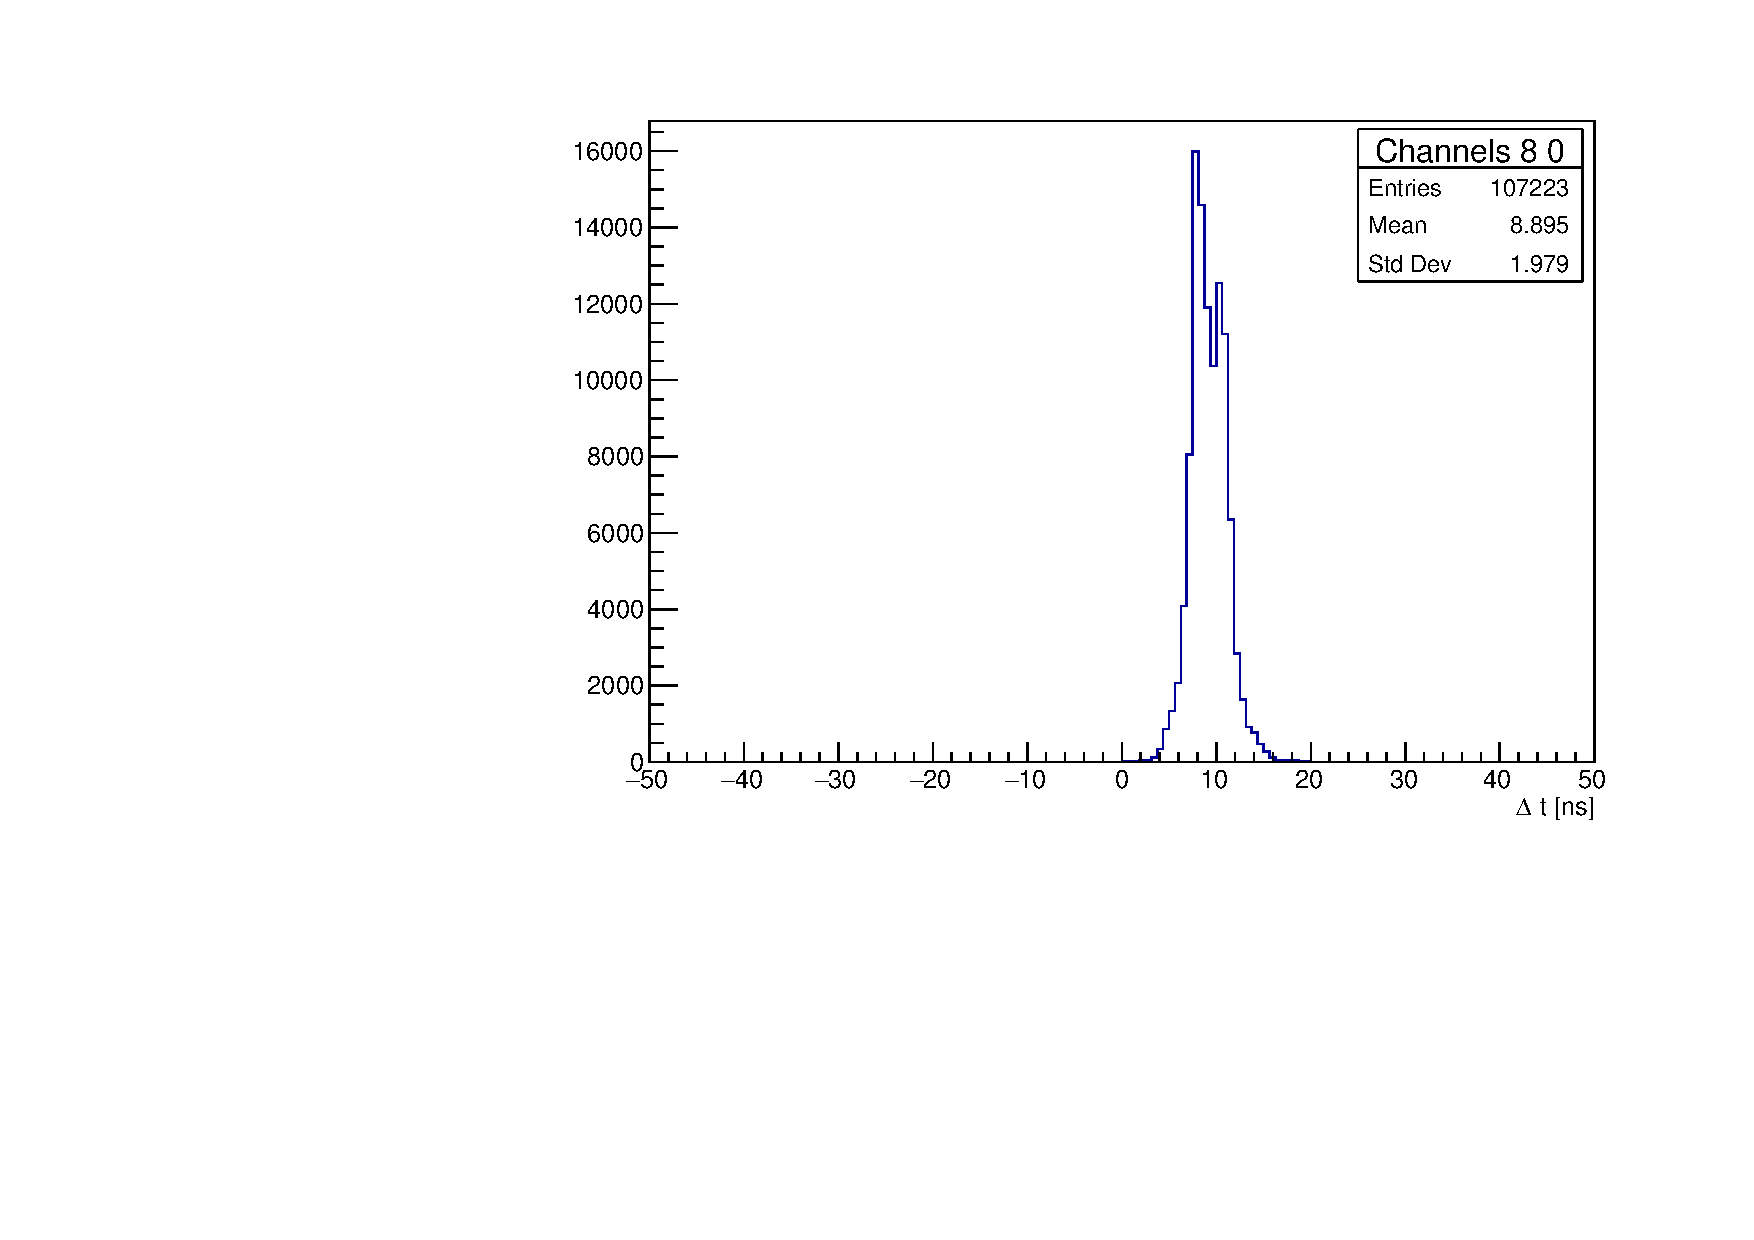
\includegraphics[width=0.49\textwidth]{figures/timingPlots/intraSlice/Channels_8_0.pdf}~
    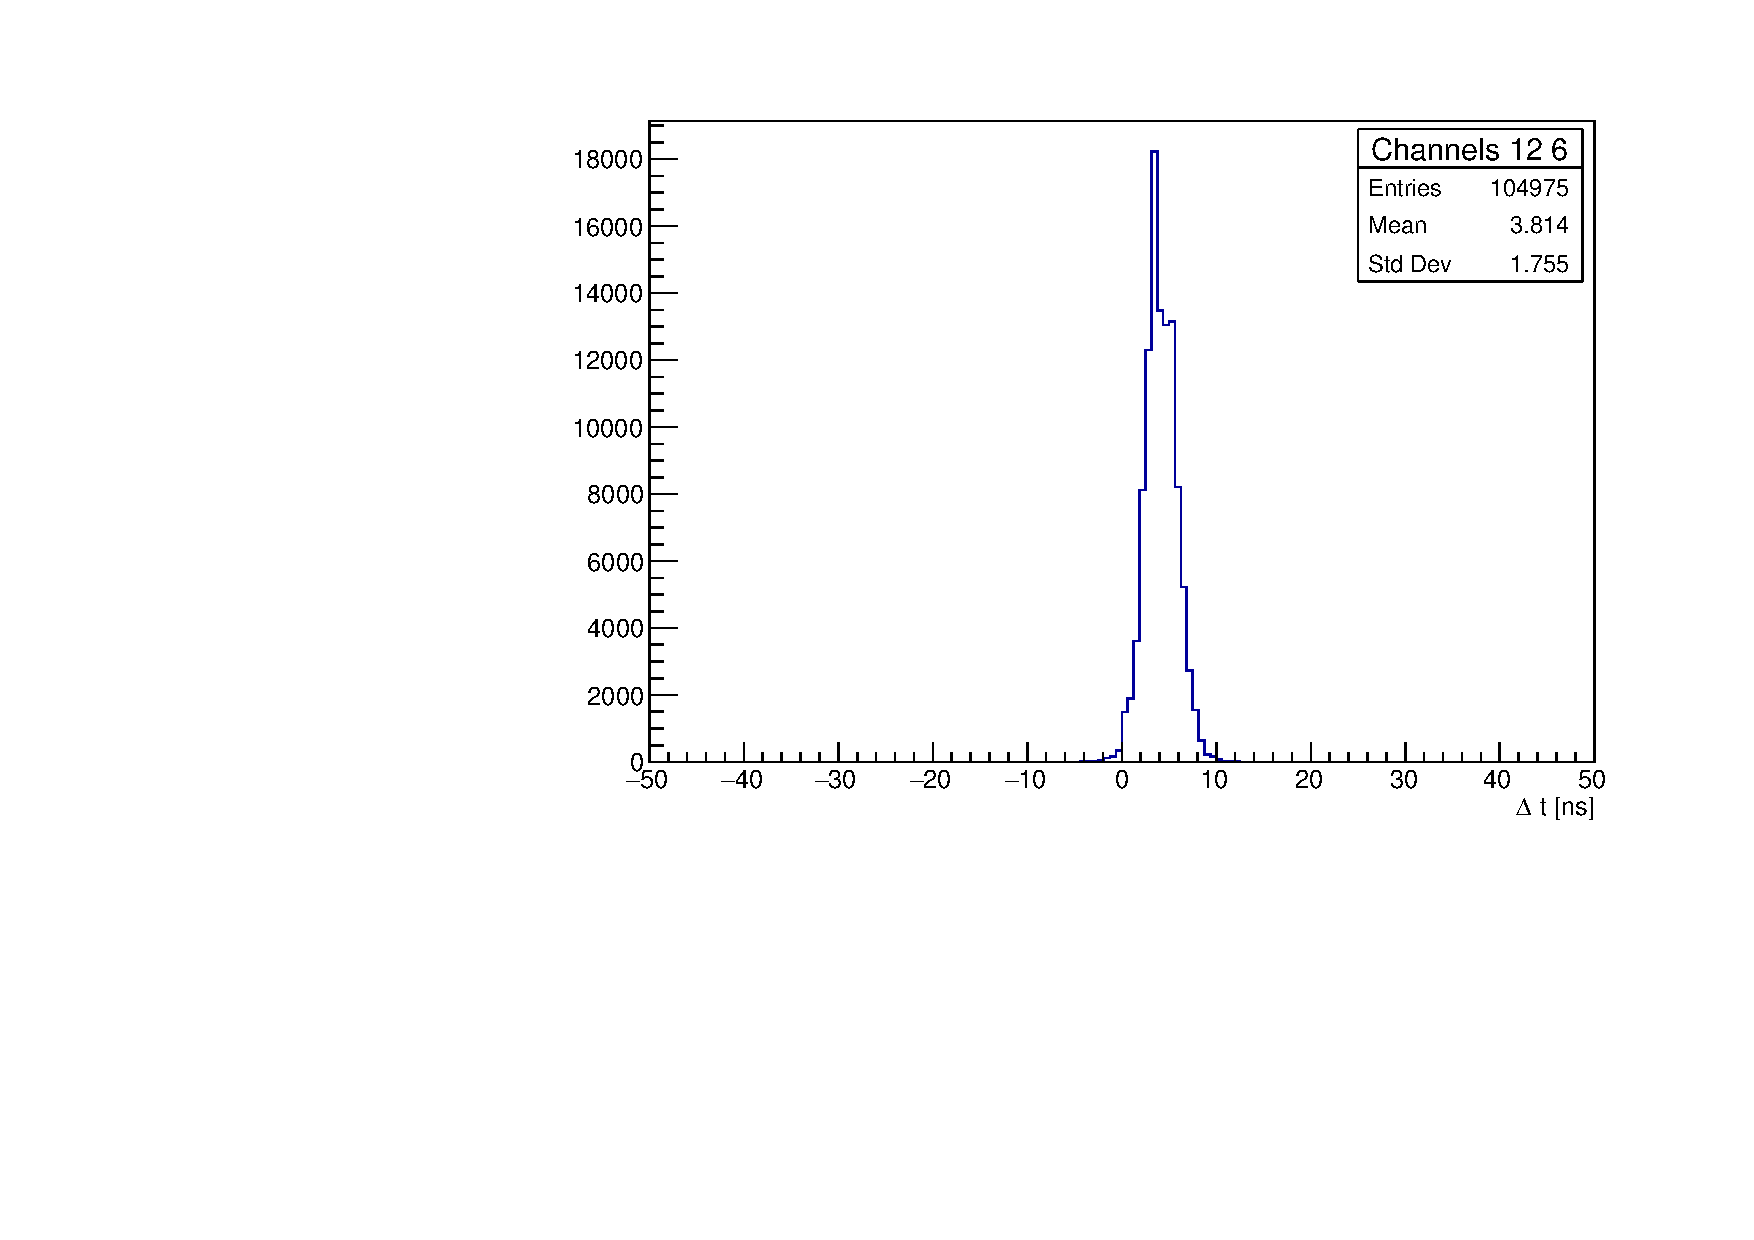
\includegraphics[width=0.49\textwidth]{figures/timingPlots/intraSlice/Channels_12_6.pdf}\\
    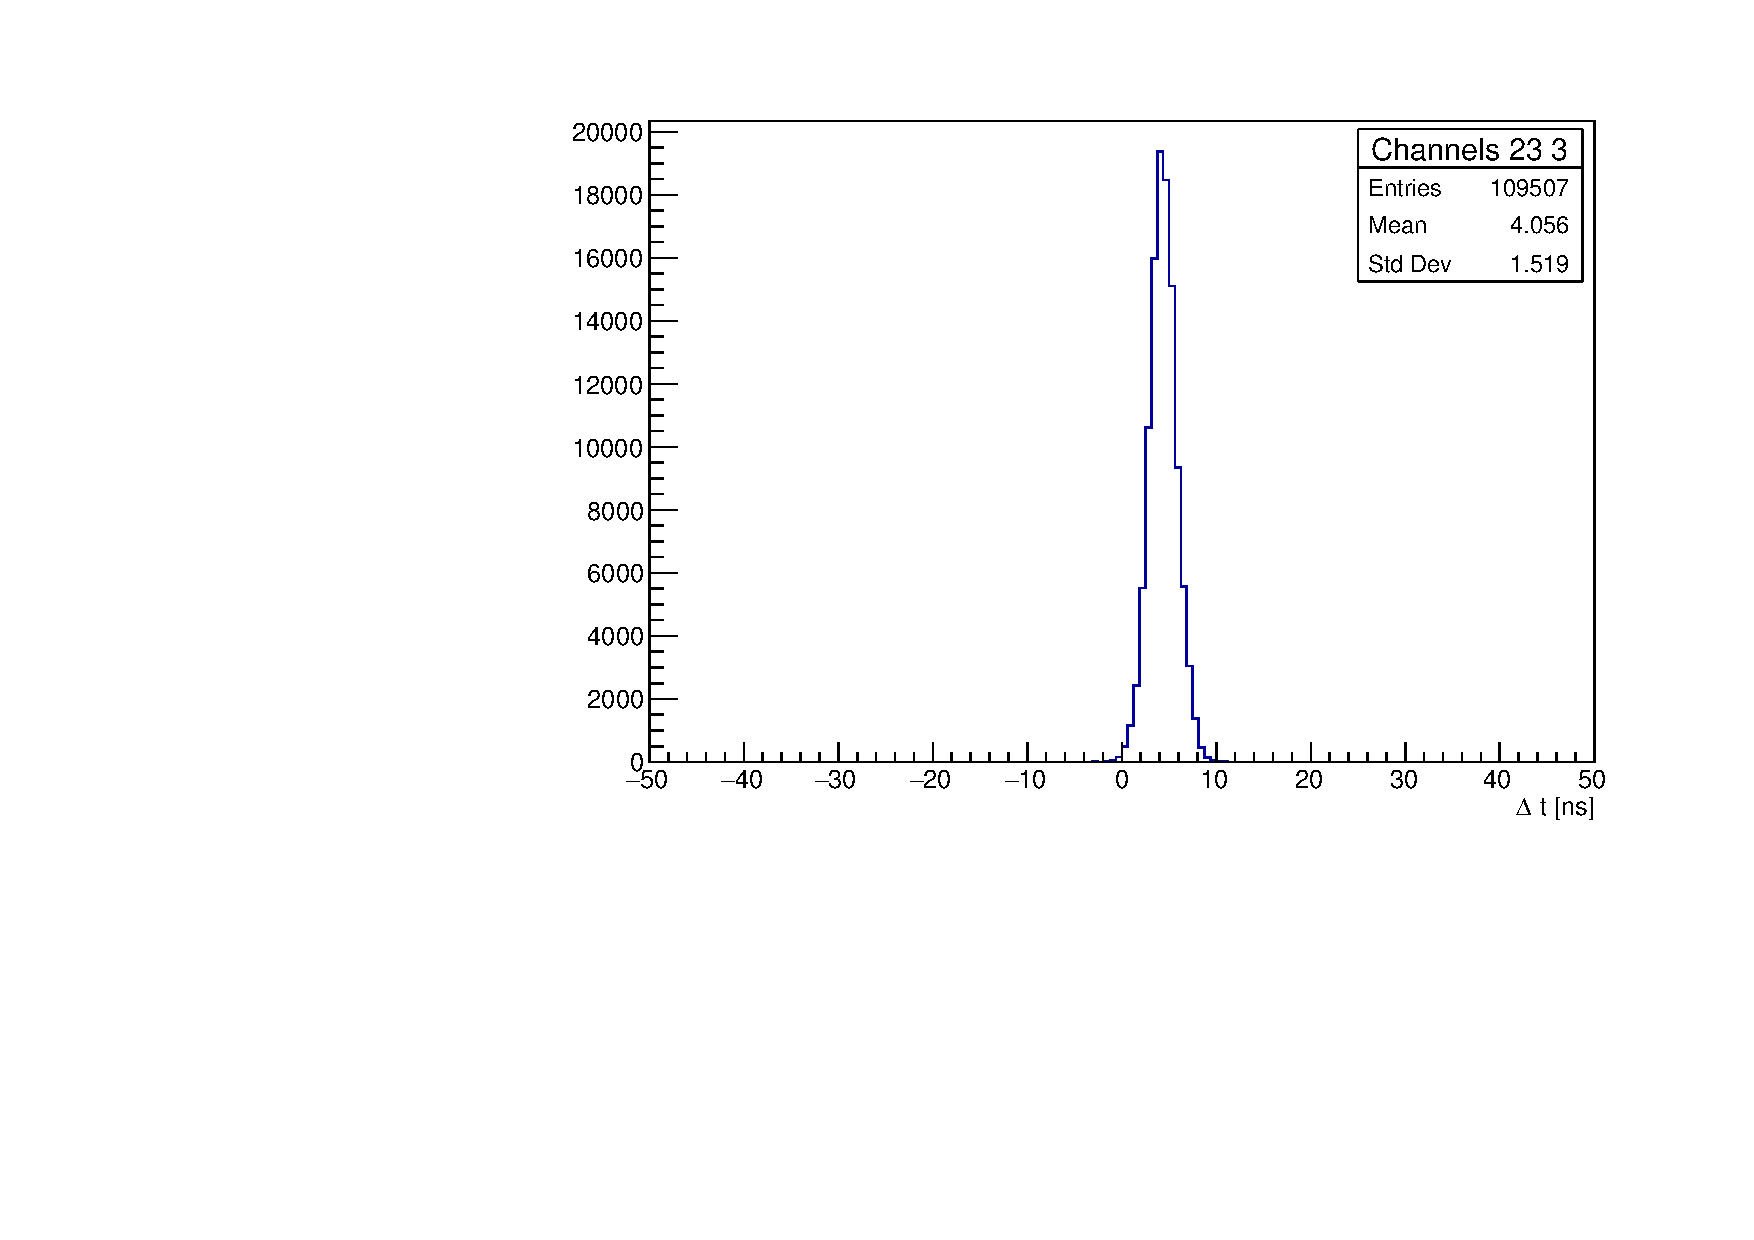
\includegraphics[width=0.49\textwidth]{figures/timingPlots/intraSlice/Channels_23_3.pdf}~
    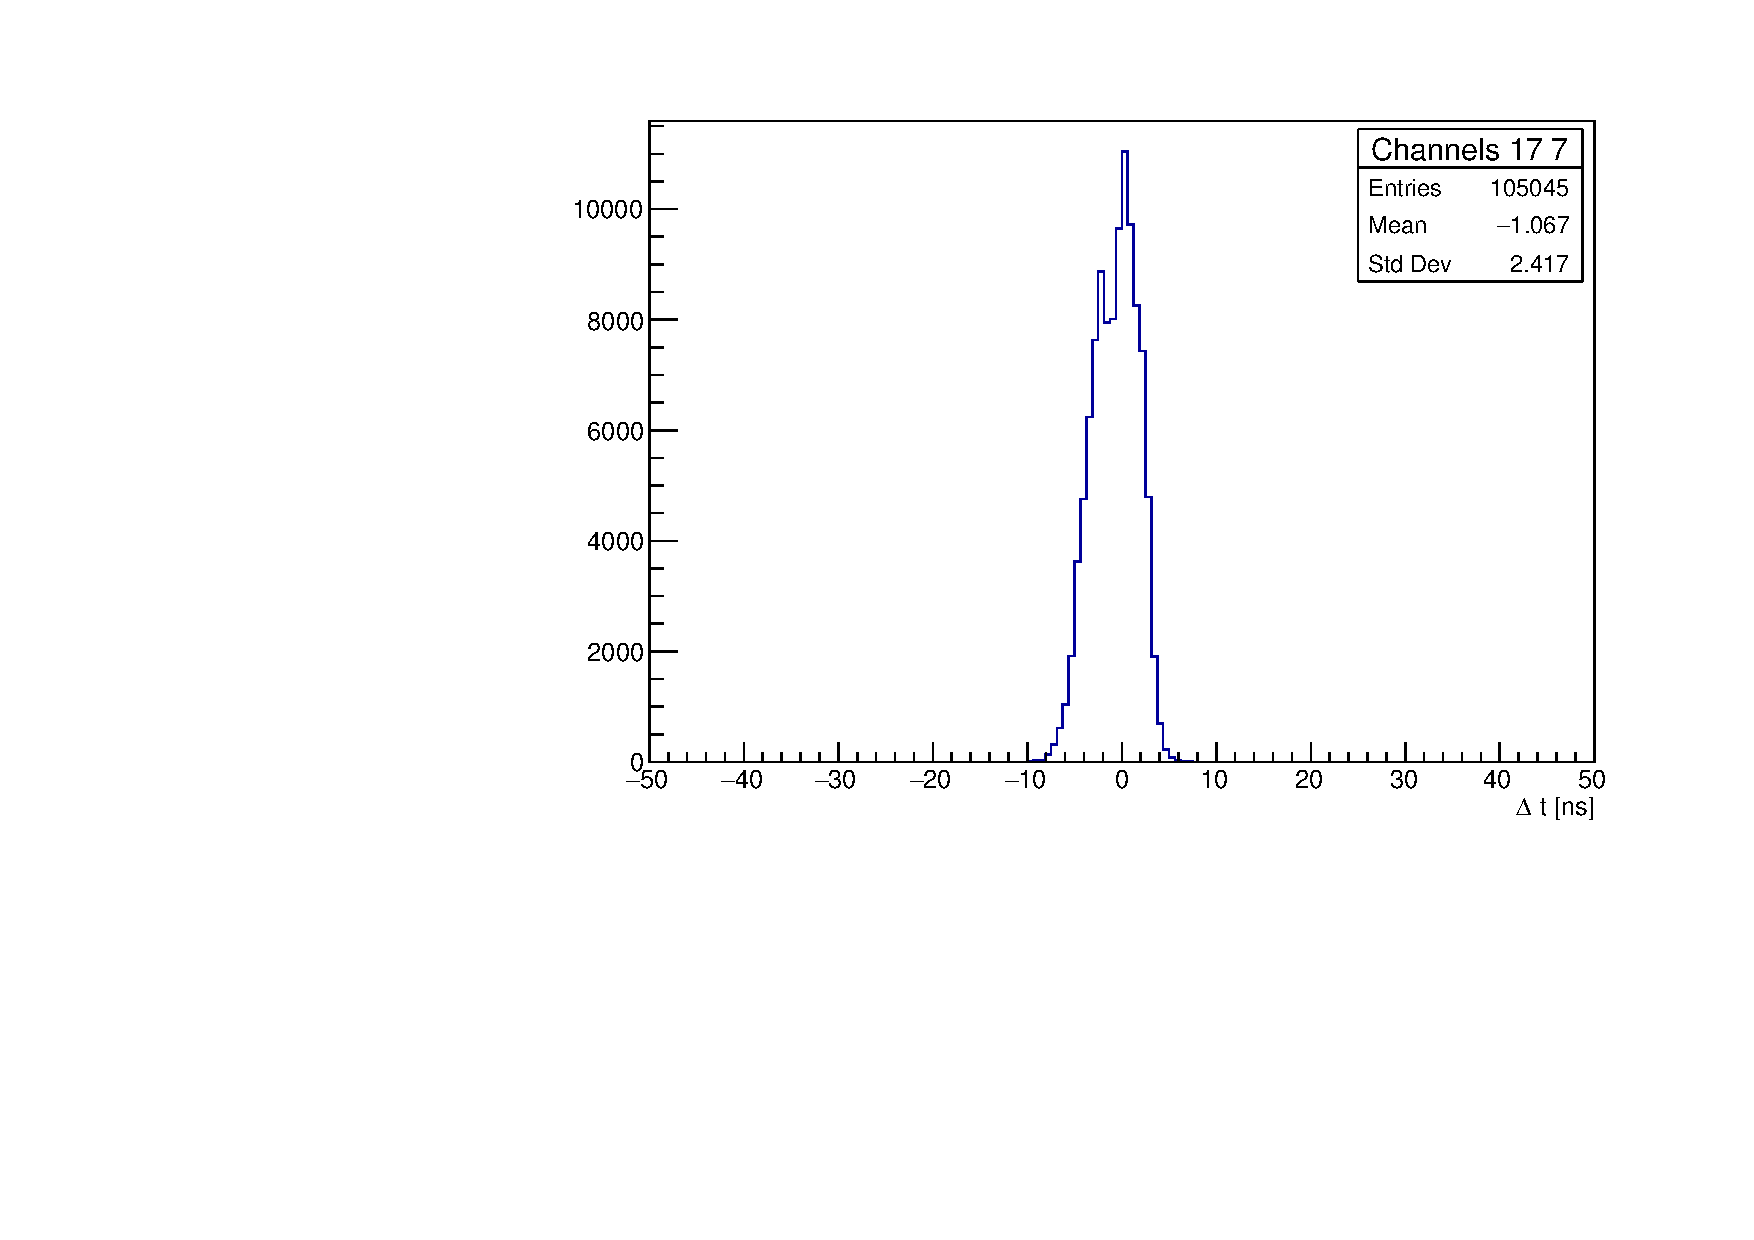
\includegraphics[width=0.49\textwidth]{figures/timingPlots/intraSlice/Channels_17_7.pdf}
    \caption{\label{fig:timeDiffIntraSlice} Example time differences between channels in the same slices. The mean values are used to calibrate the intra-slice timing.}
\end{figure}

After applying the intra-slice calibration, the slices are then calibrated using down-going cosmic muons, tagged as muon pulse hitting the top panel and both slices in a particular layer.
The mean value of the time difference relative to the left slice of each layer is taken as the calibration.
Figure~\ref{fig:timeDiffIntraLayer} shows the time difference between the slices for each layer.
The standard deviation ranges from 2.3 to 2.8\unit{ns}.

\begin{figure}
    \centering
    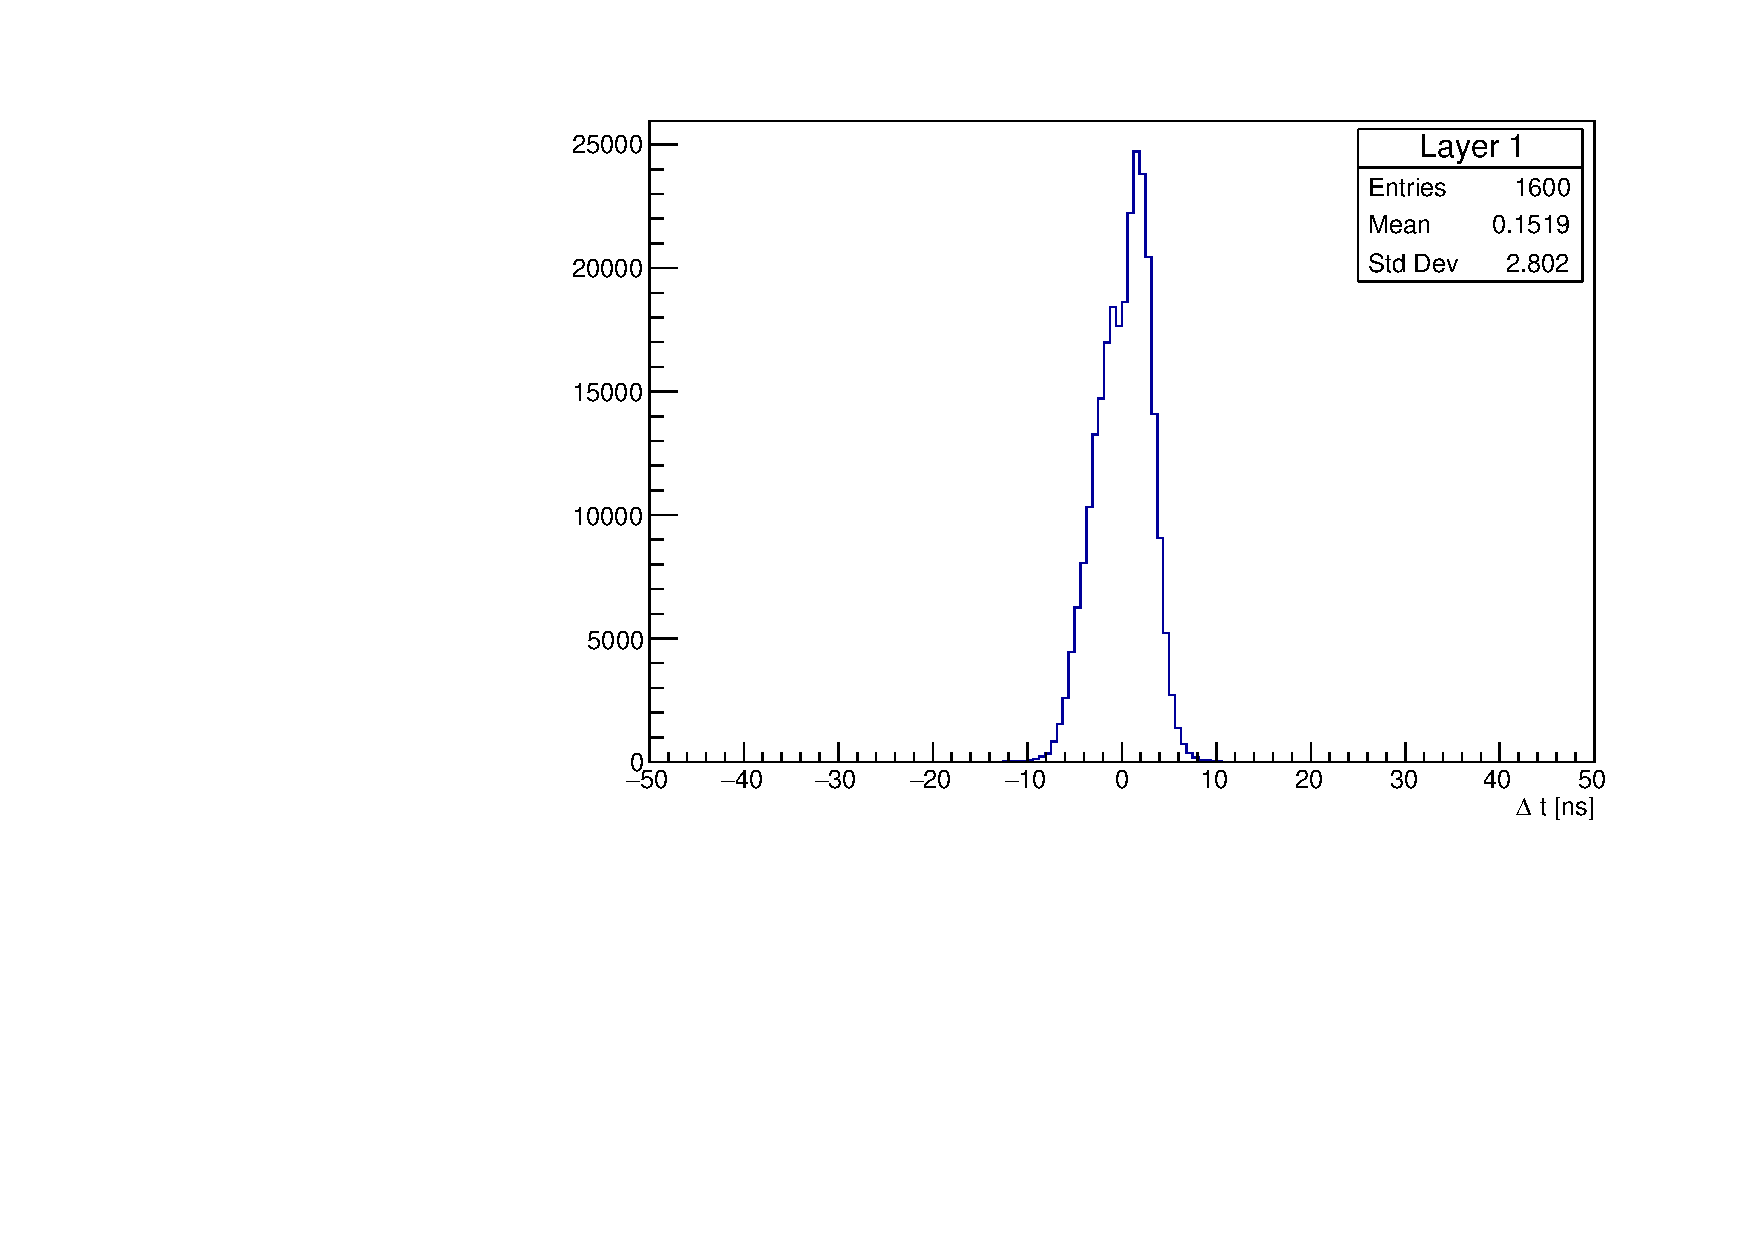
\includegraphics[width=0.49\textwidth]{figures/timingPlots/intraLayer/Layer_1.pdf}~
    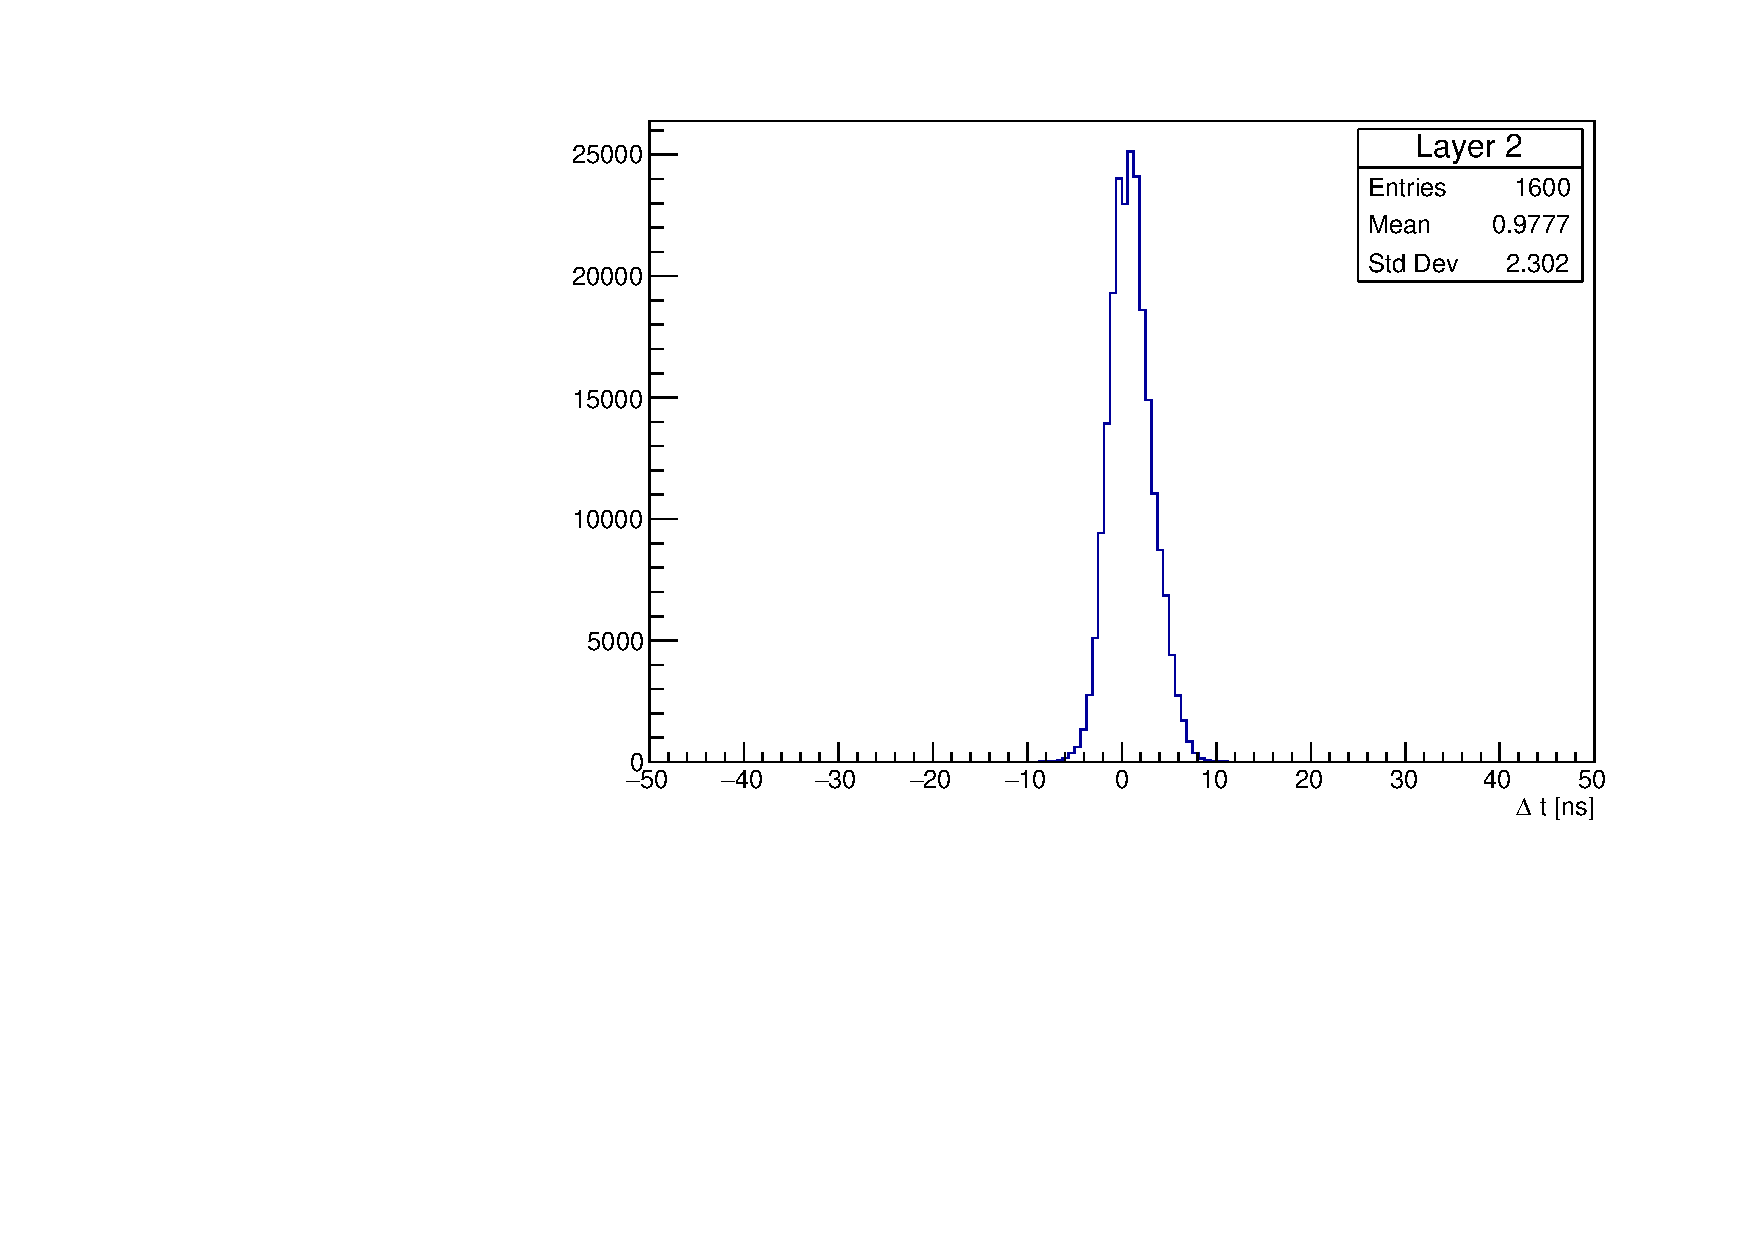
\includegraphics[width=0.49\textwidth]{figures/timingPlots/intraLayer/Layer_2.pdf}\\
    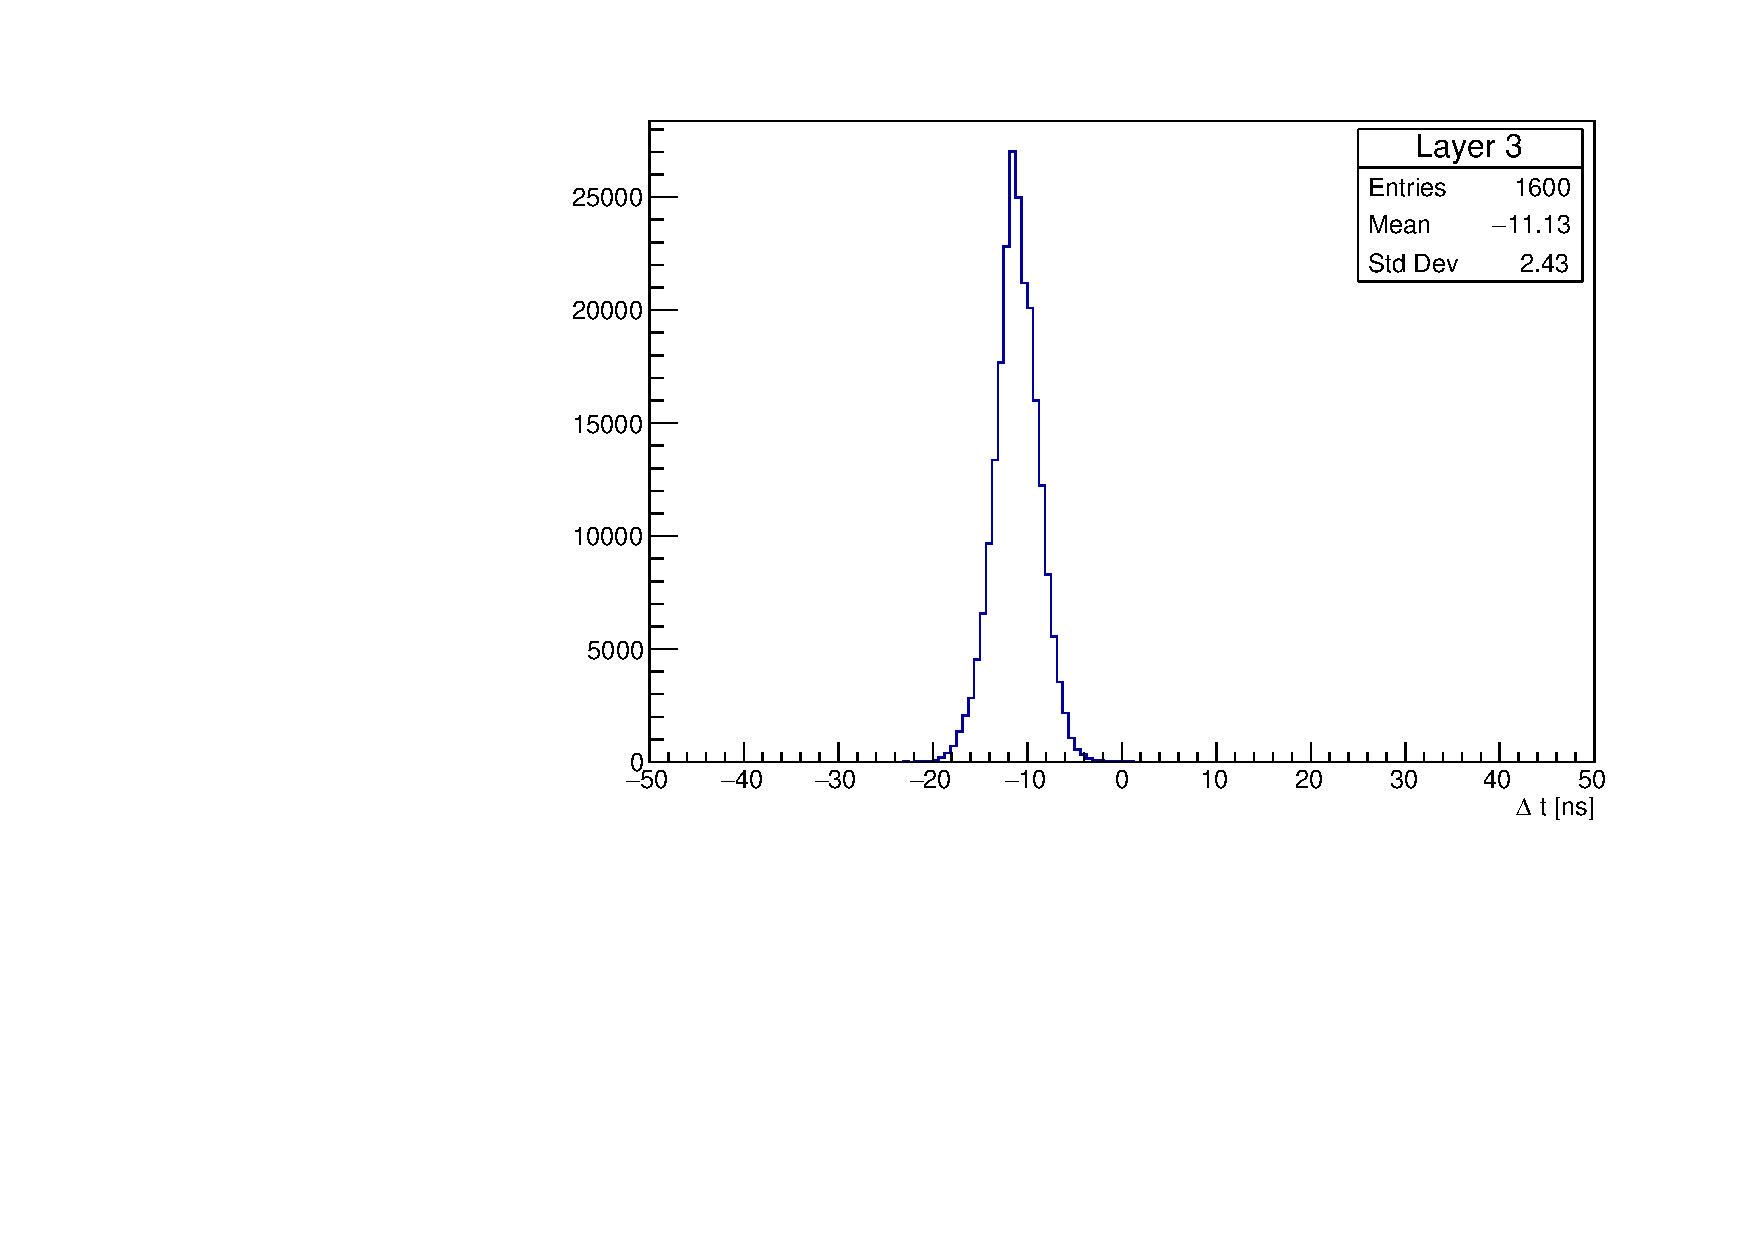
\includegraphics[width=0.49\textwidth]{figures/timingPlots/intraLayer/Layer_3.pdf}
    \caption{\label{fig:timeDiffIntraLayer} Time differences between slices in the same layer for all layers. The mean values are used to calibrate the intra-layer timing.}
\end{figure}

The slab timing is then calibrated using beam muons, tagged as a muon pulse 
hitting all four slabs. In order to avoid bias from cosmic muons, the modal 
value of the time difference relative to the slab closest to the CMS IP (channel 18) 
is taken as the calibration. Figure~\ref{fig:timeDiffInterSlab} shows
the time difference between the slabs and channel 18. 

\begin{figure}
    \centering
    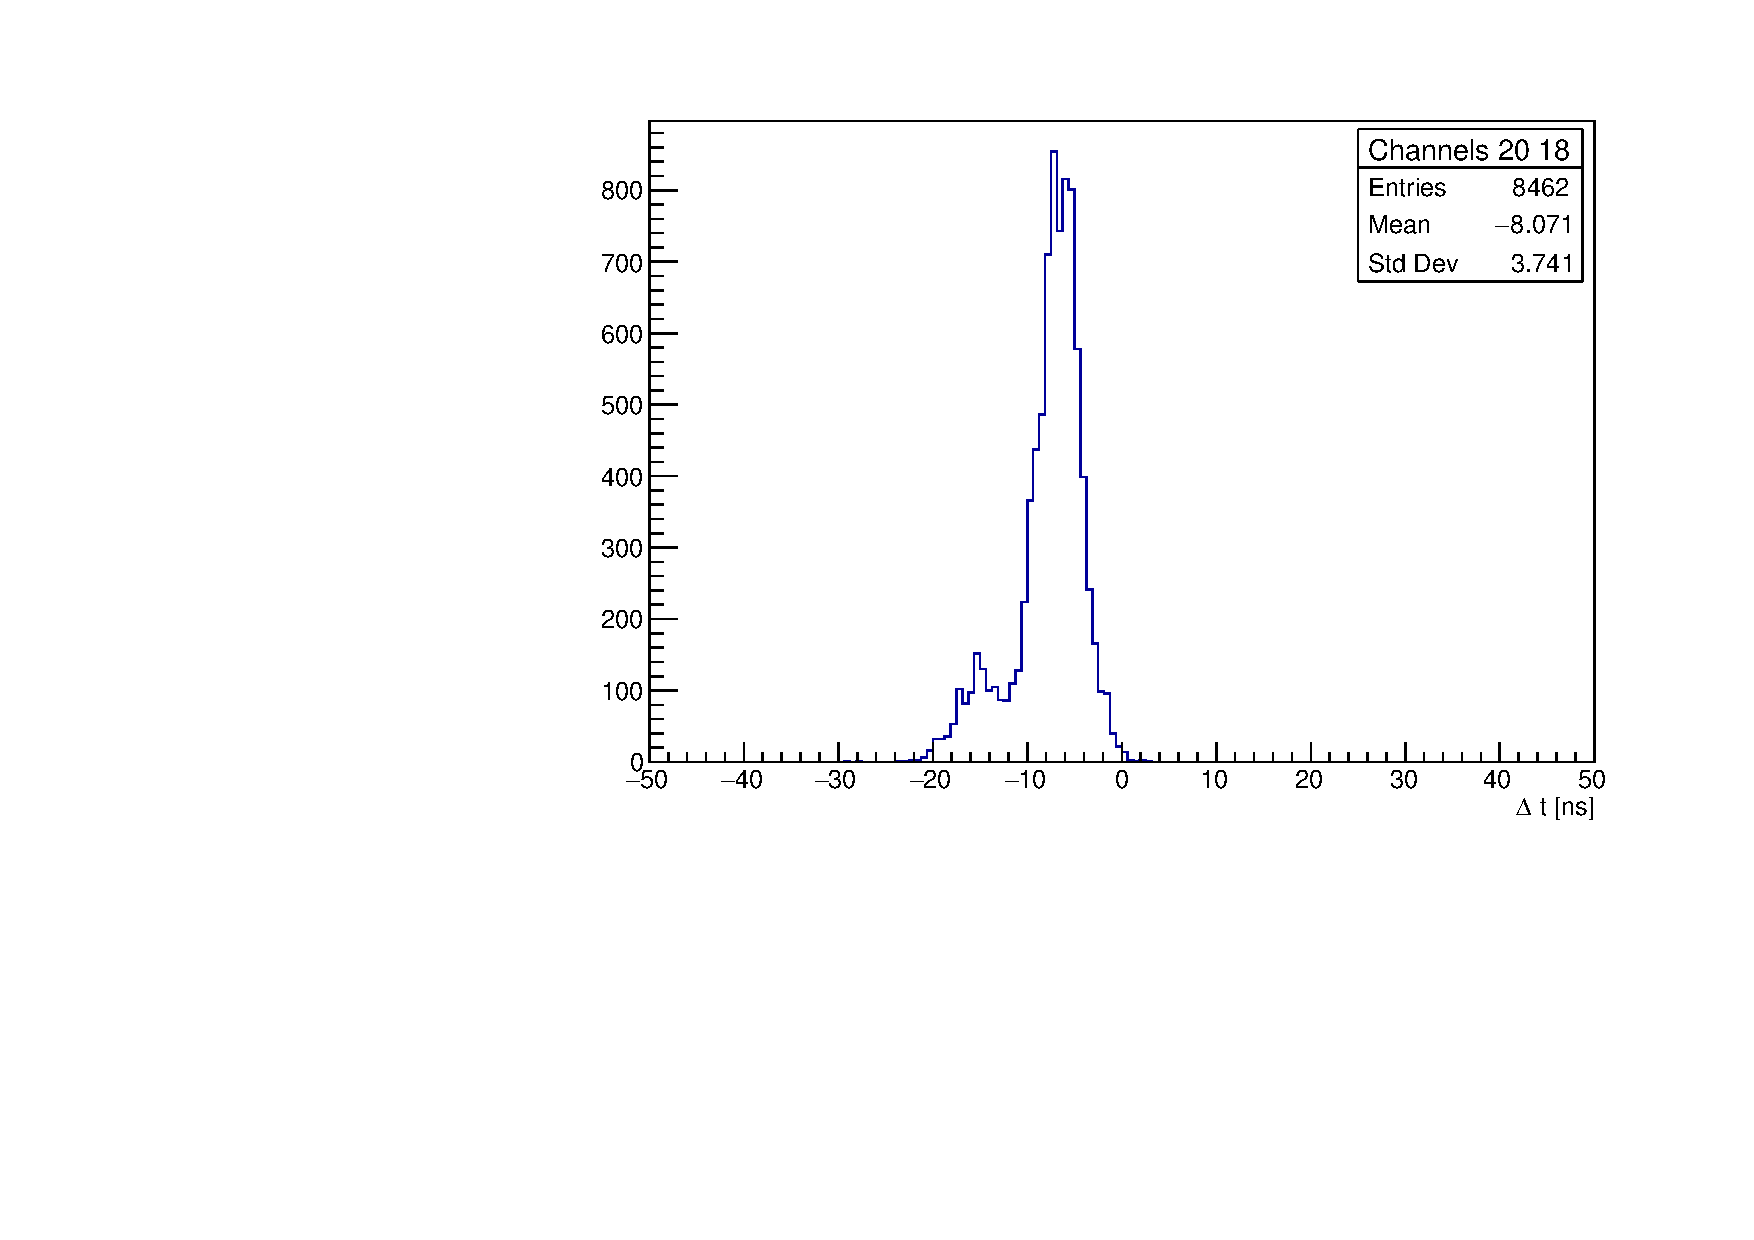
\includegraphics[width=0.49\textwidth]{figures/timingPlots/intraSlice/Channels_20_18.pdf}~
    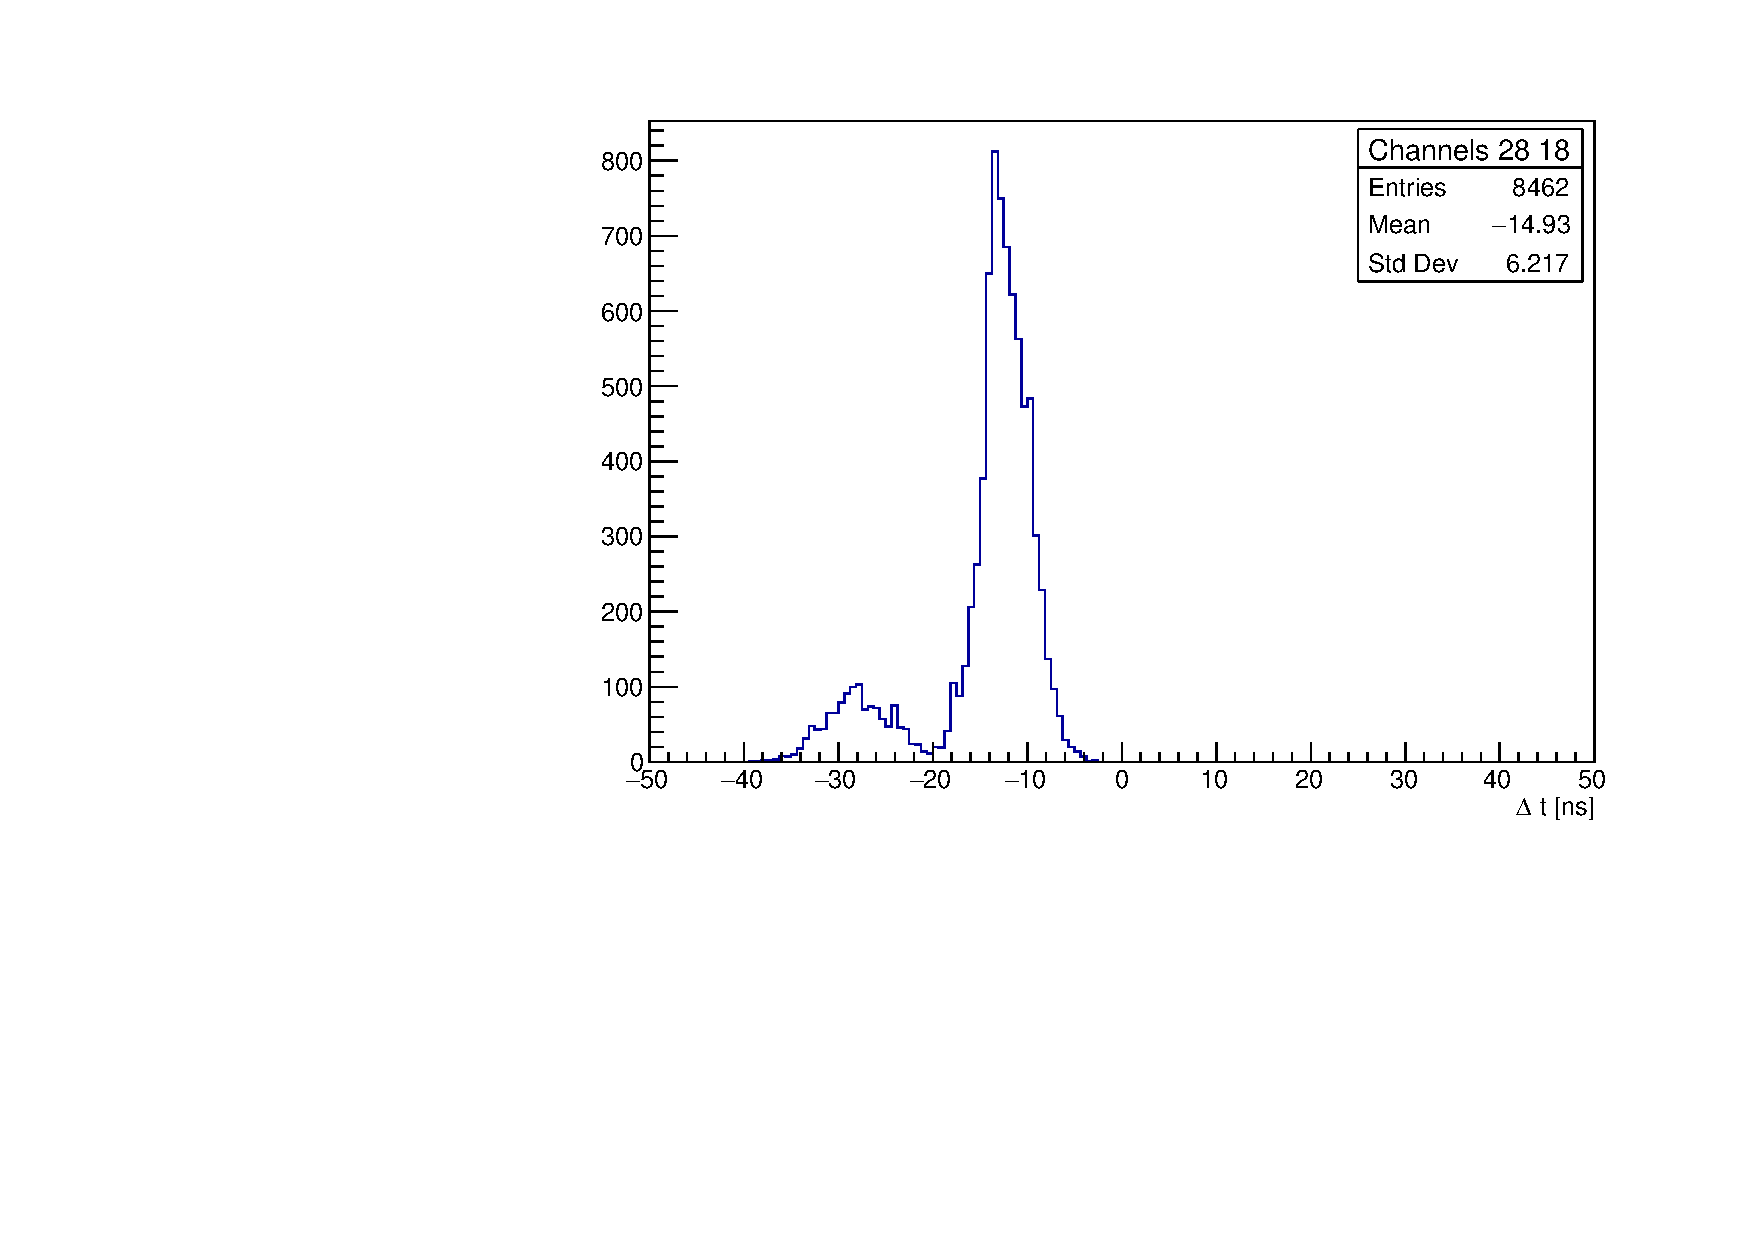
\includegraphics[width=0.49\textwidth]{figures/timingPlots/intraSlice/Channels_28_18.pdf}\\
    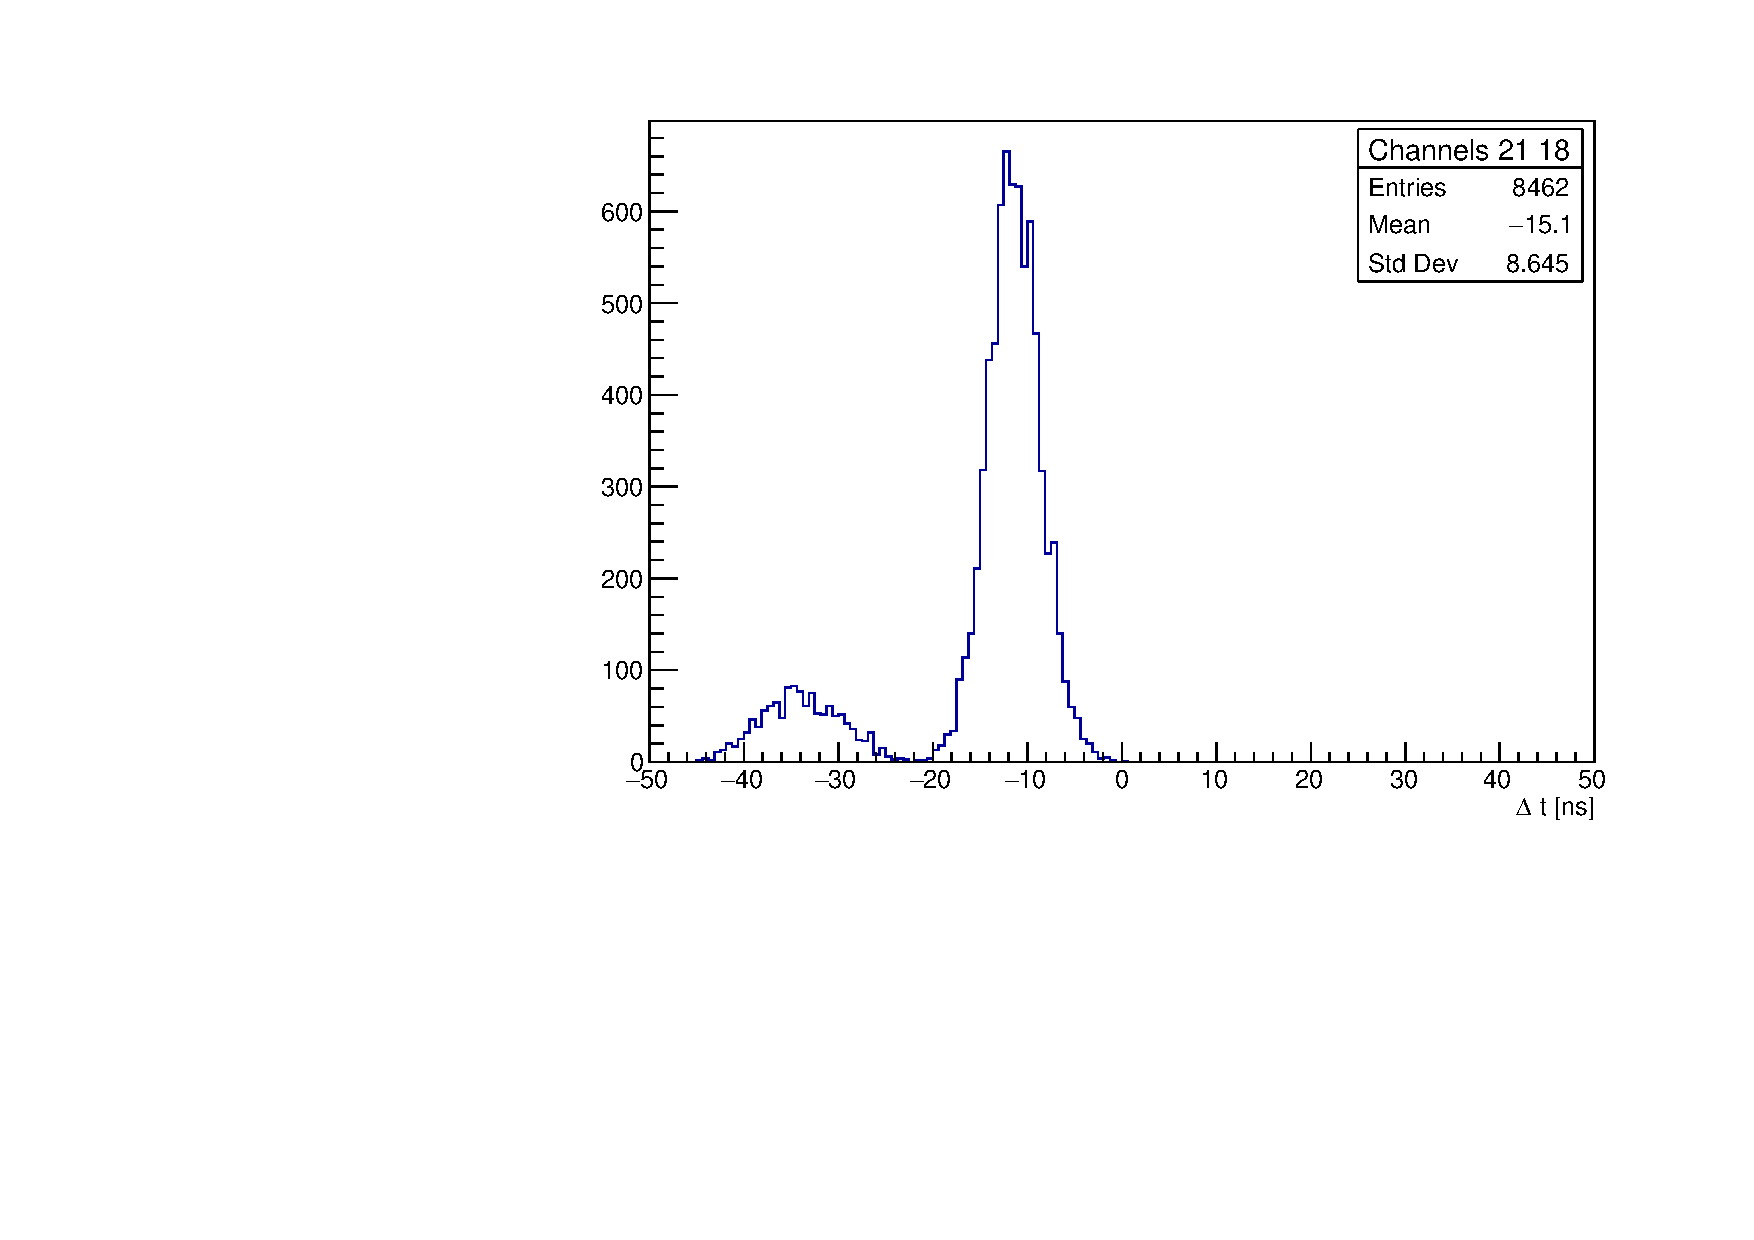
\includegraphics[width=0.49\textwidth]{figures/timingPlots/intraSlice/Channels_21_18.pdf}
    \caption{\label{fig:timeDiffInterSlab} Time differences between each slab and channel 18. 
    The modal values are used to calibrate the inter-slab timing.}
\end{figure}

After applying all previous calibrations the layers are calibrated using beam and cosmic muons hitting all 
four layers, tagged as a muon pulse hitting all four slabs. The mean value of the time difference
relative to the slab closest to the layer is taken as the calibration. Figure~\ref{fig:timeDiffInterLayer}
shows the time difference between the layers and closest slab. The standard deviation ranges from
4.3 to 4.8\unit{ns}.

\begin{figure}
    \centering
    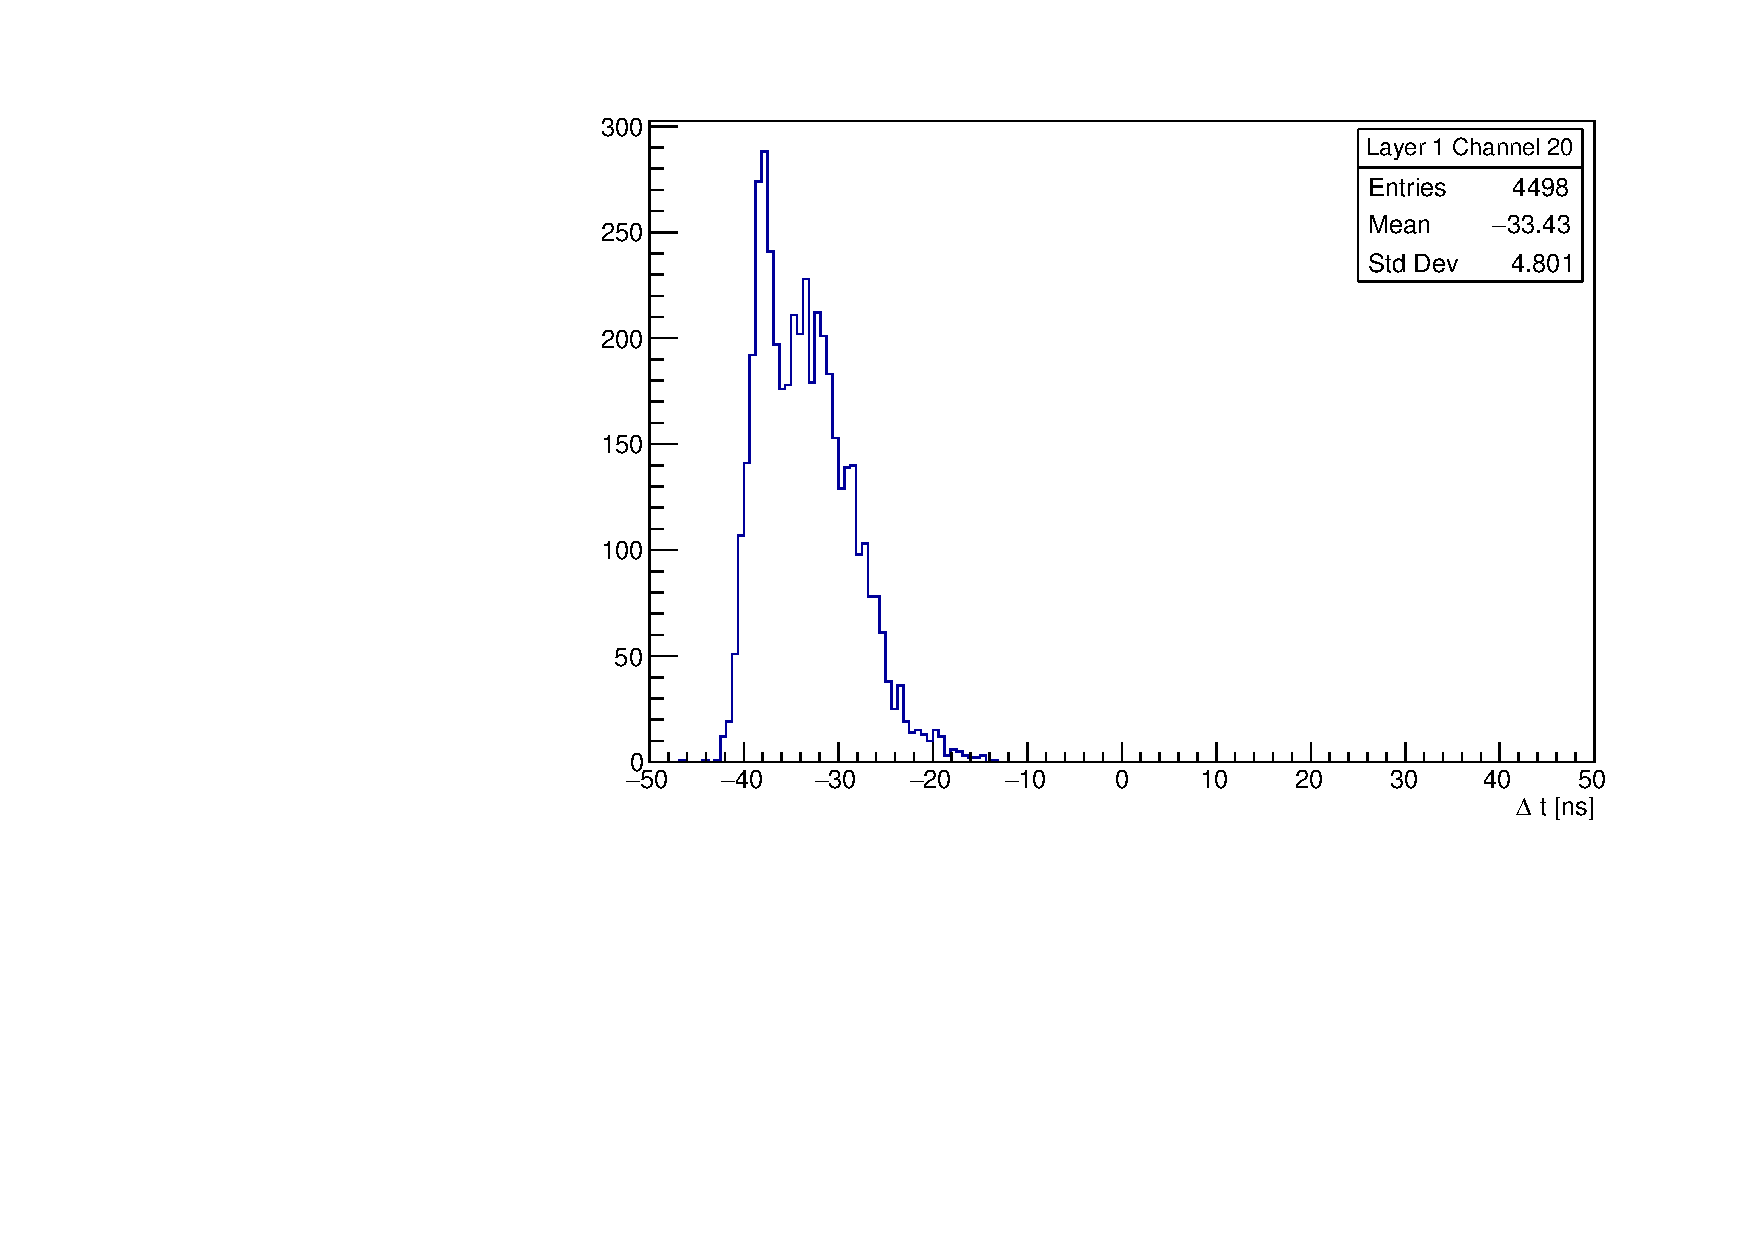
\includegraphics[width=0.49\textwidth]{figures/timingPlots/interLayer/Layer_1_Channel_20.pdf}~
    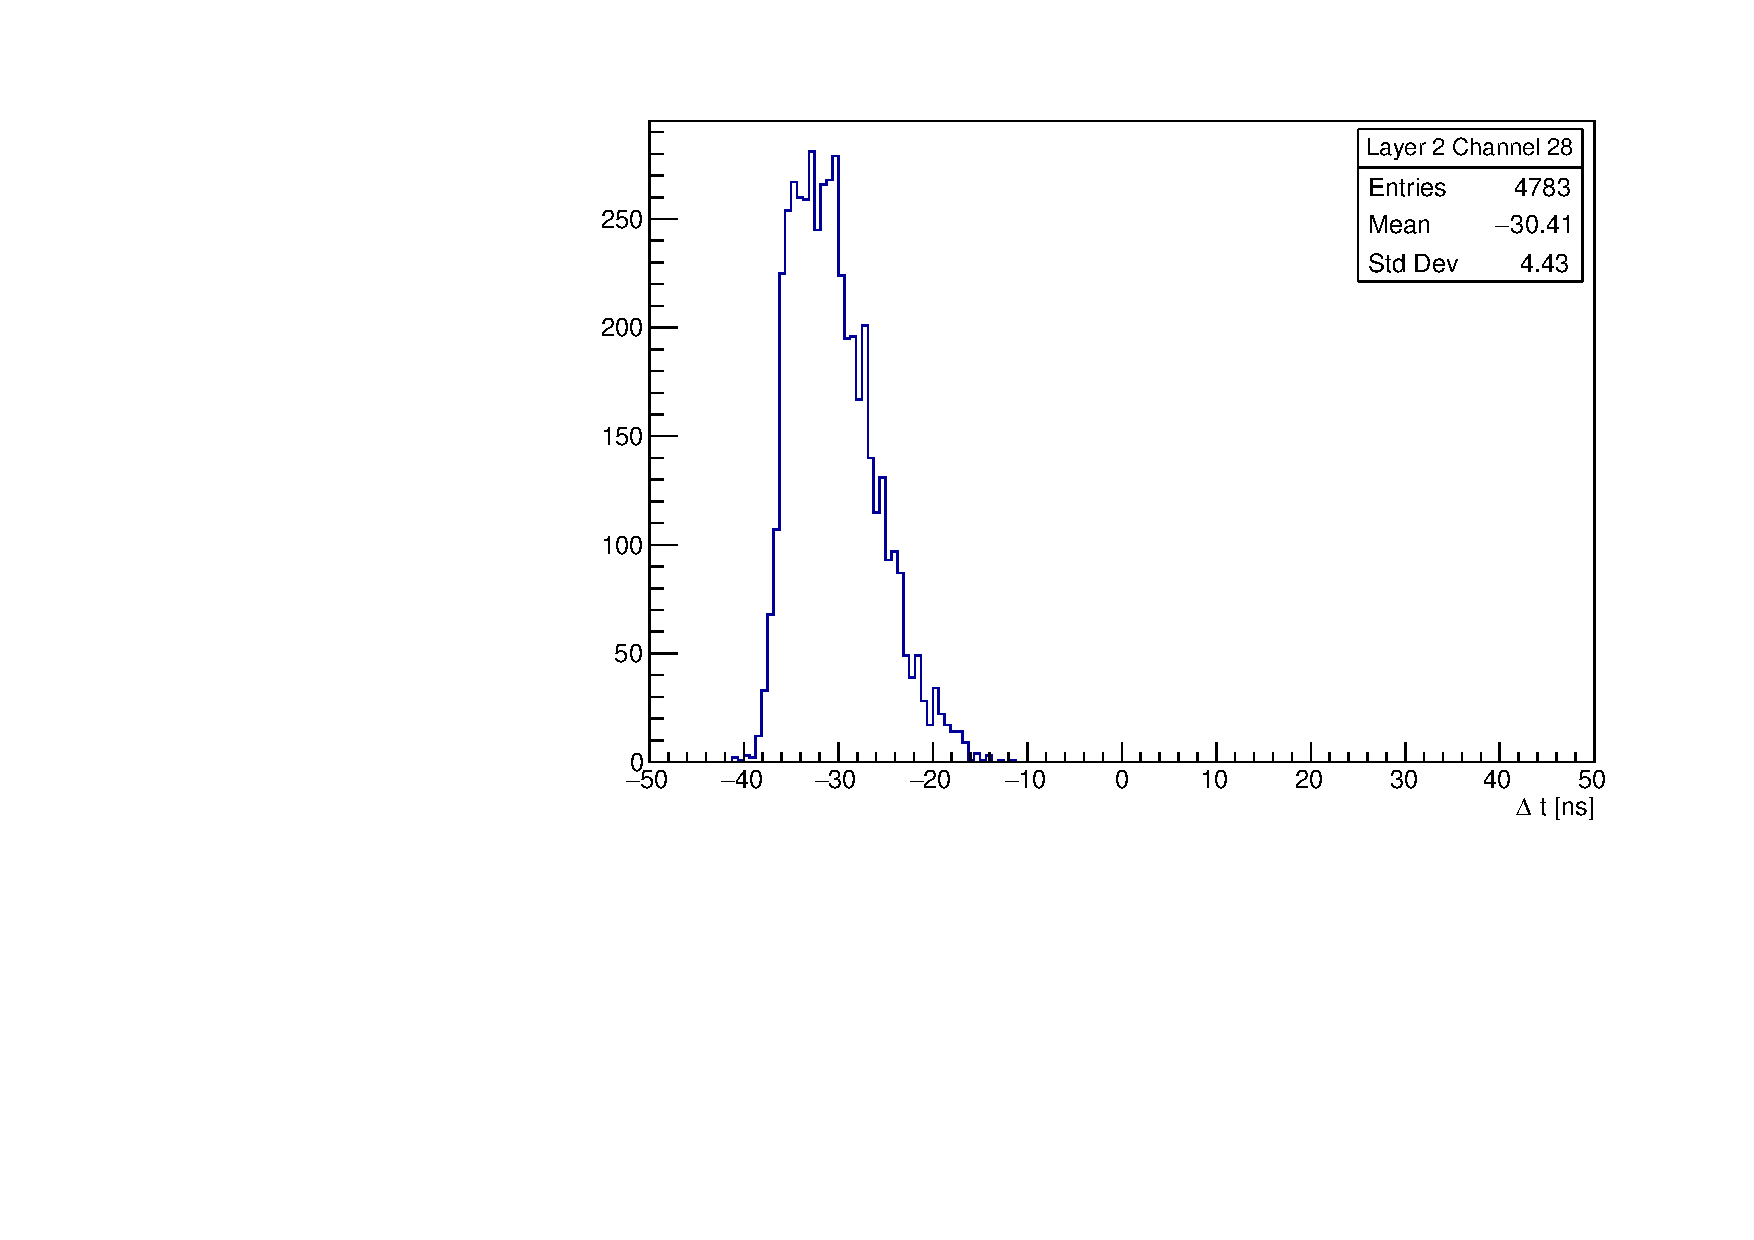
\includegraphics[width=0.49\textwidth]{figures/timingPlots/interLayer/Layer_2_Channel_28.pdf}\\
    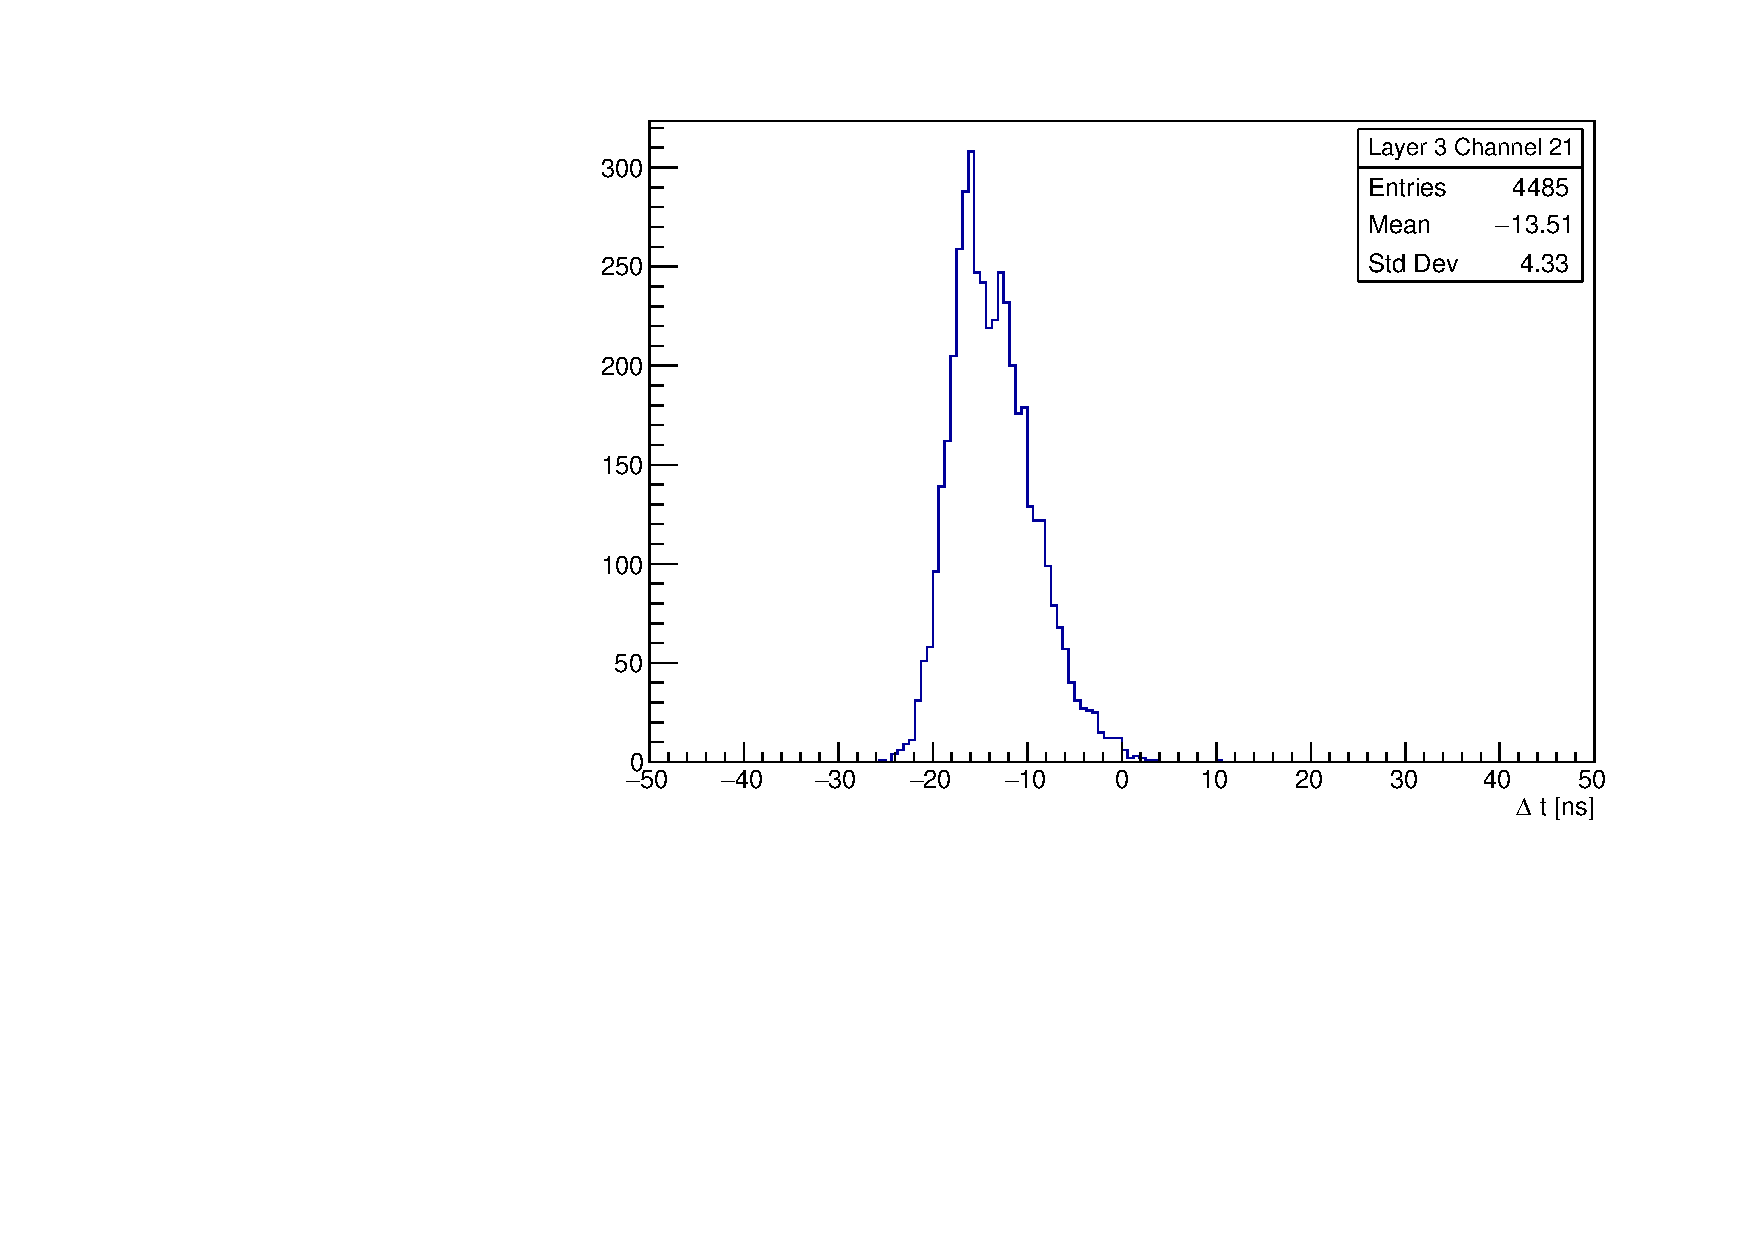
\includegraphics[width=0.49\textwidth]{figures/timingPlots/interLayer/Layer_3_Channel_21.pdf}
    \caption{\label{fig:timeDiffInterLayer} Example time differences between each layer and the closest slab. 
    The mean values are used to calibrate the inter-layer timing.}
\end{figure}

Finally, the panels are calibrated to the layers using cosmic muons tagged as having a muon
pulse in the panel and in the layer closest to the panel. The mean value of the time 
difference relative to the layer is taken as the calibration. Figure~\ref{fig:timeDiffPanelLayer}
shows representative time differences between the panels and the closest layer. The standard deviation ranges
from 5.8 to 8.0\unit{ns}.

\begin{figure}
    \centering
    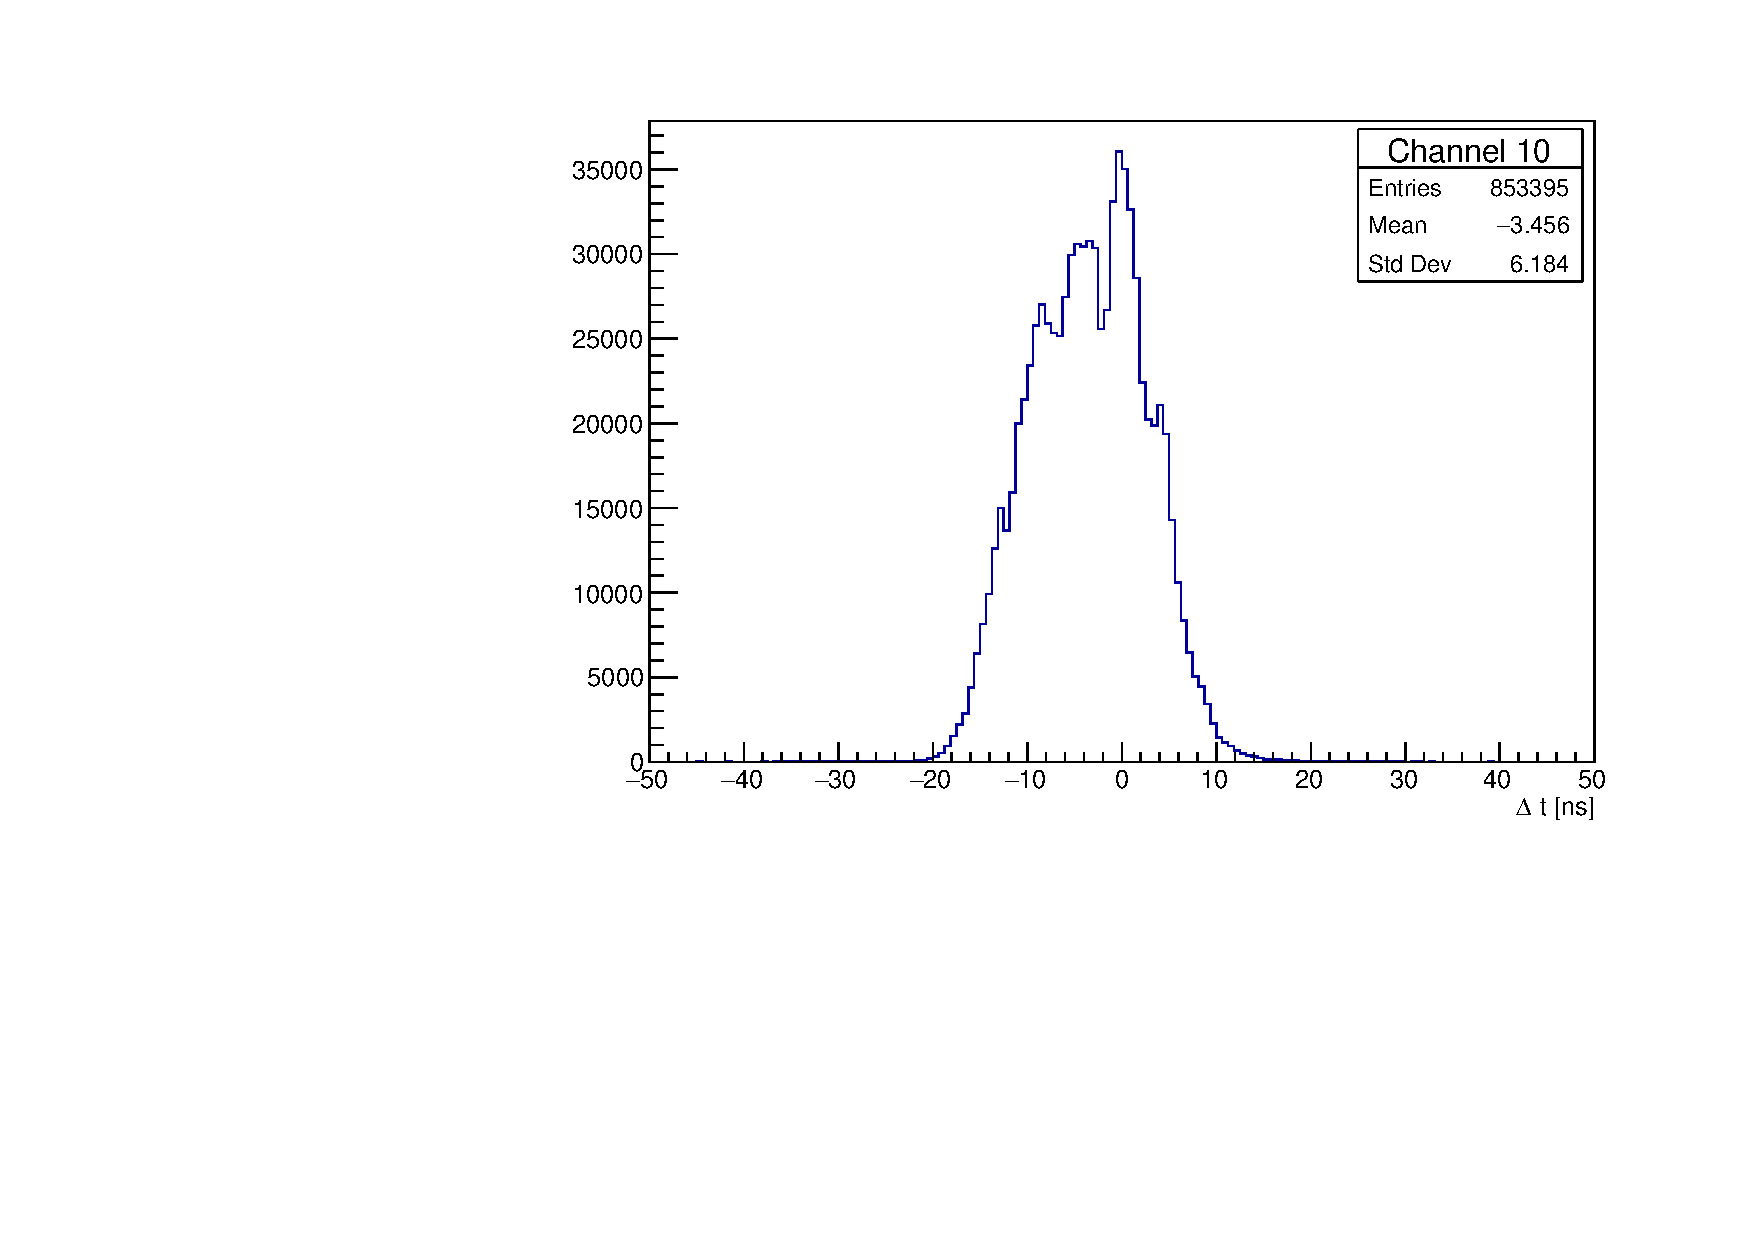
\includegraphics[width=0.49\textwidth]{figures/timingPlots/panels/Channel_10.pdf}~
    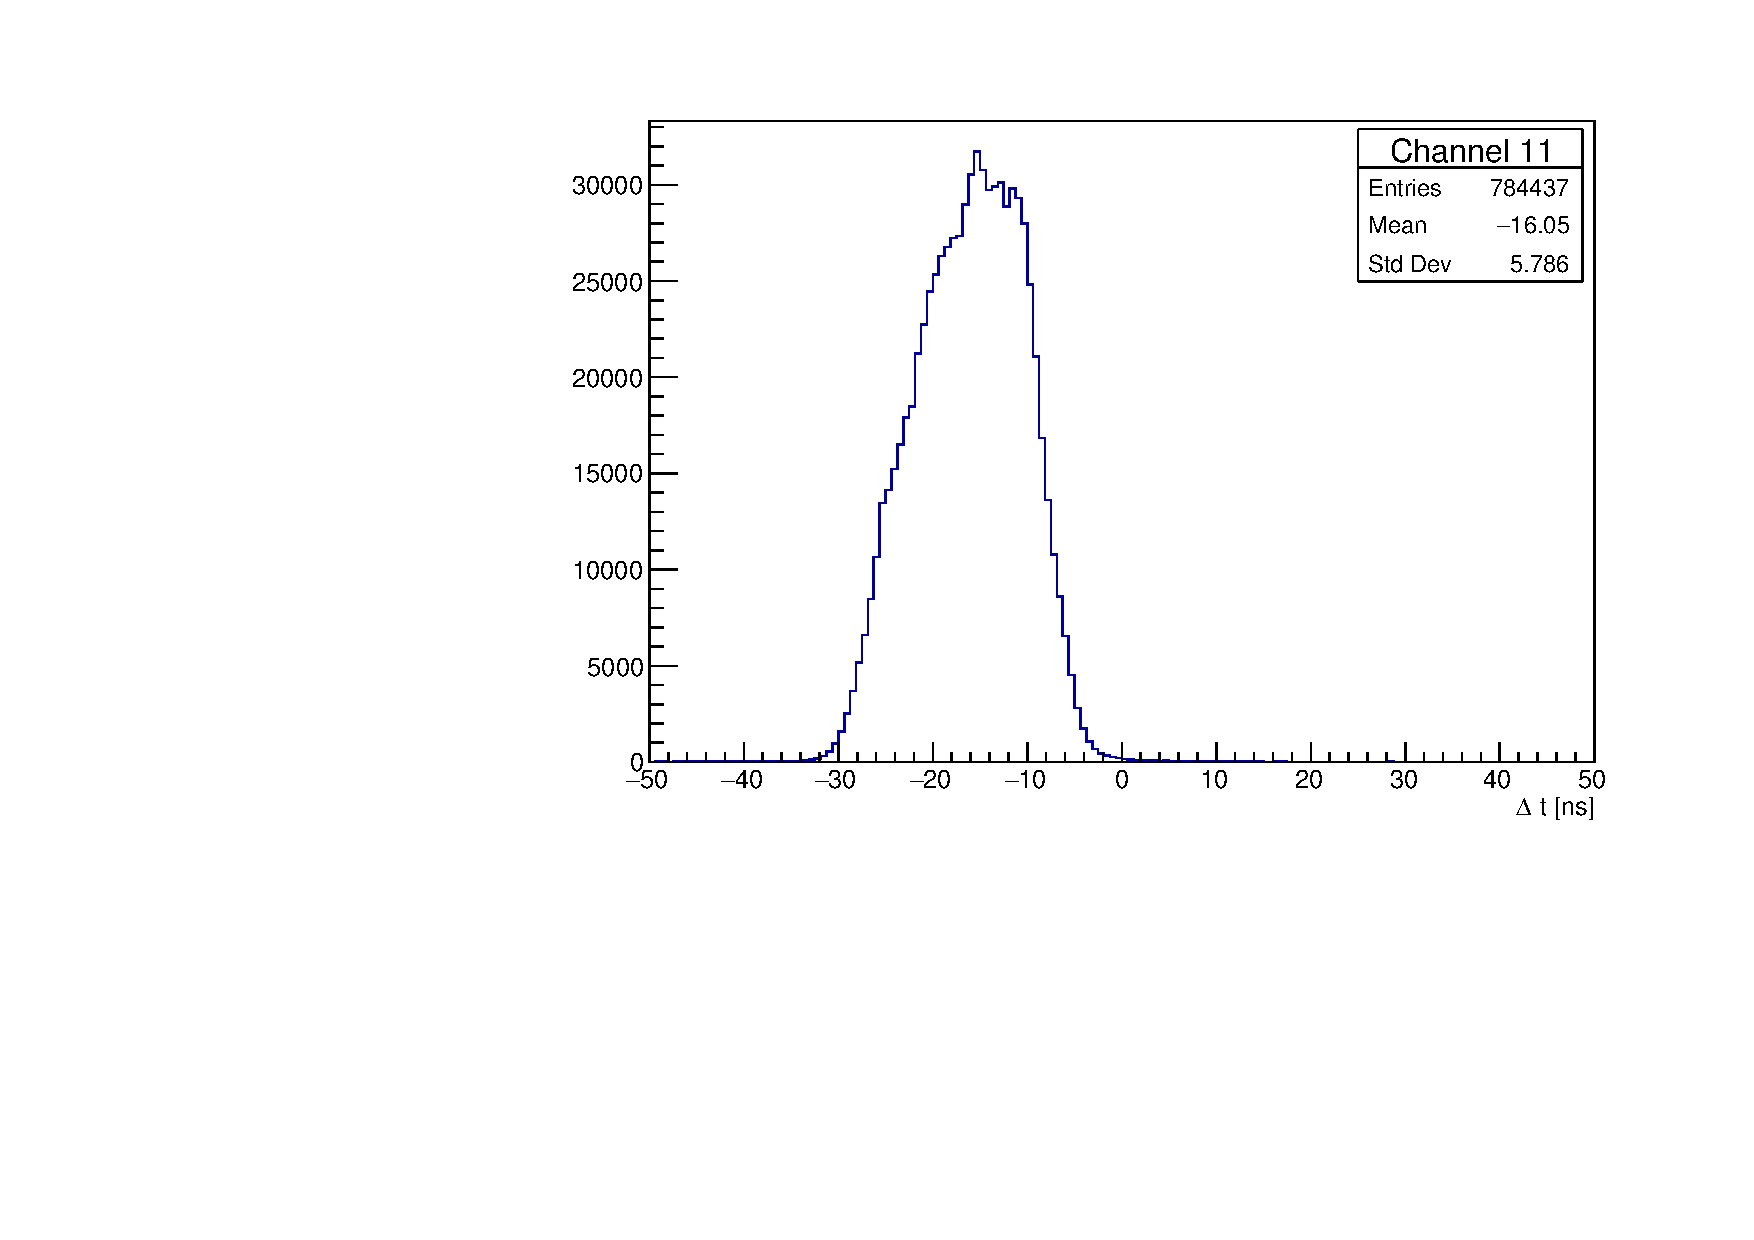
\includegraphics[width=0.49\textwidth]{figures/timingPlots/panels/Channel_11.pdf}\\
    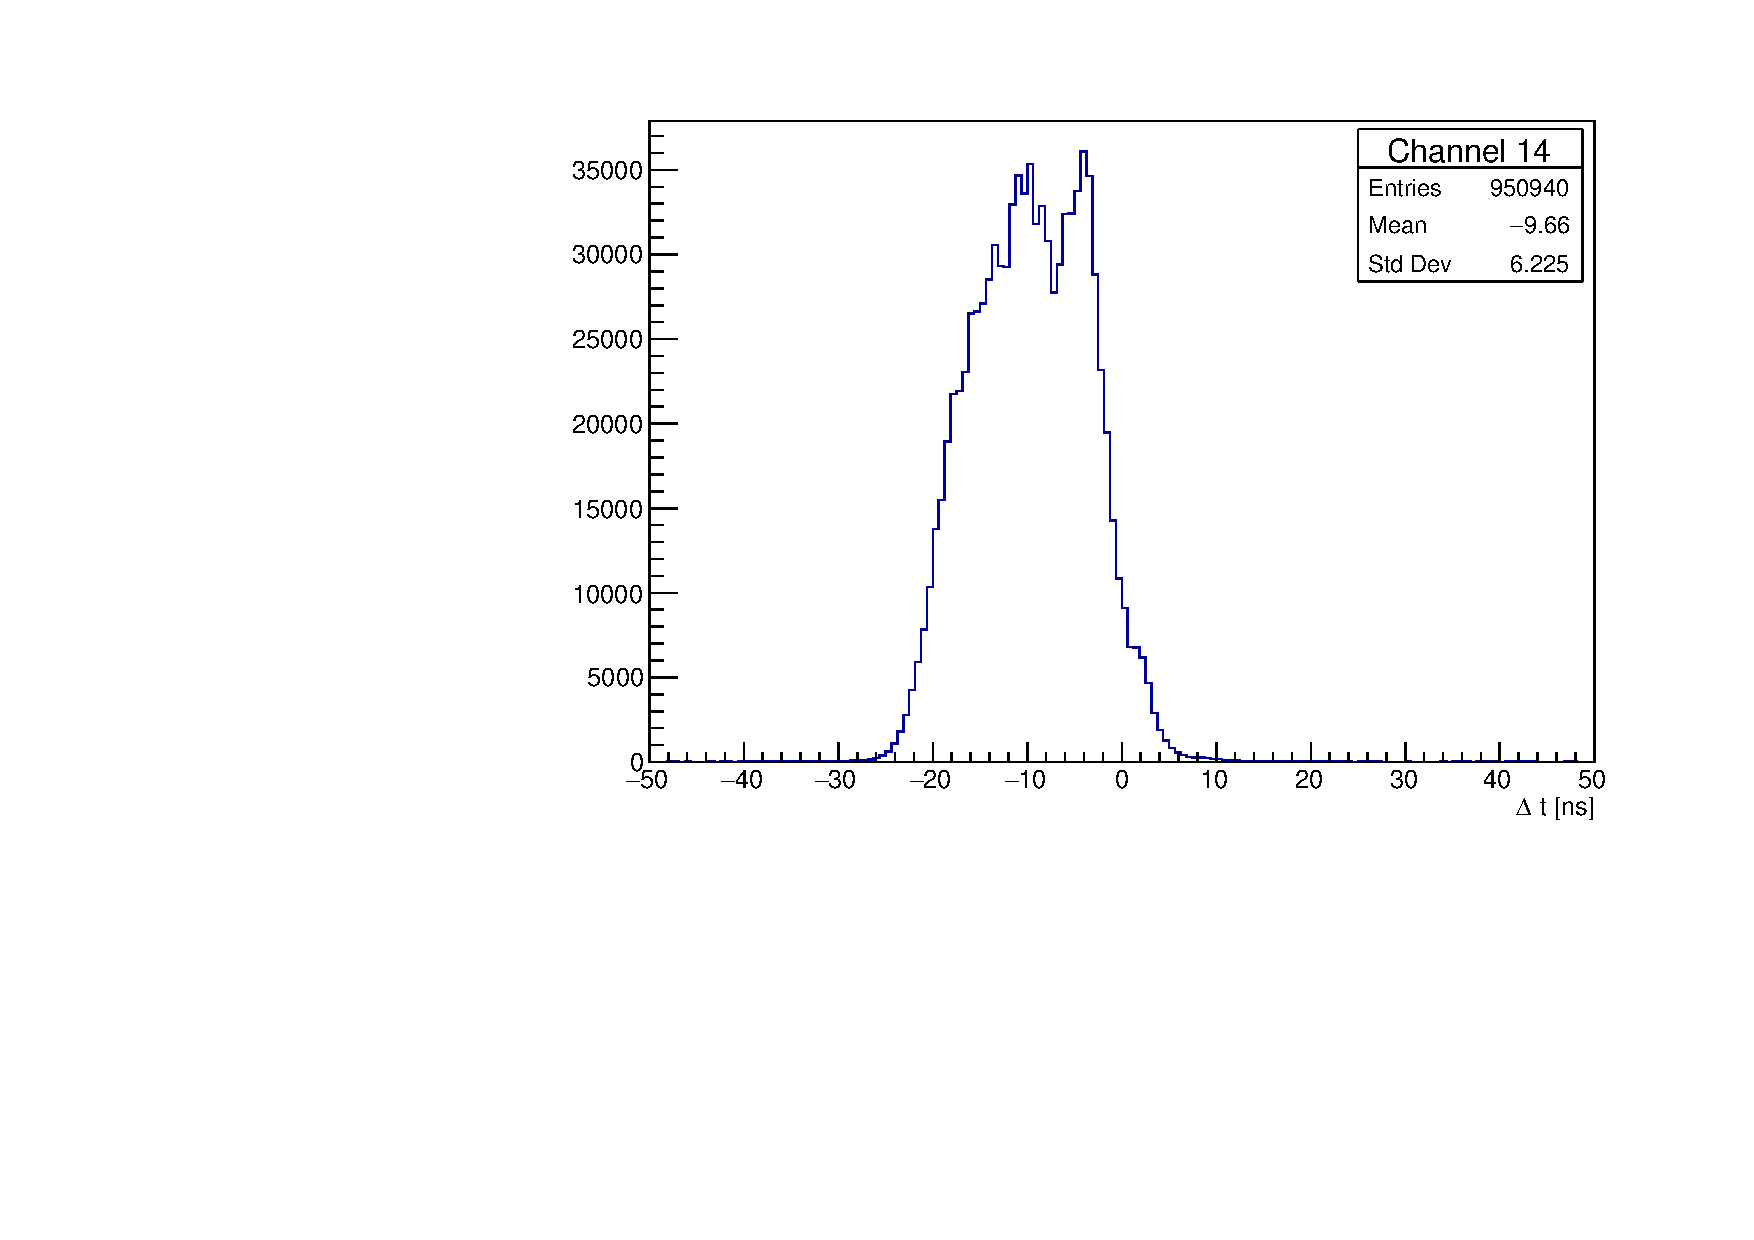
\includegraphics[width=0.49\textwidth]{figures/timingPlots/panels/Channel_14.pdf}~
    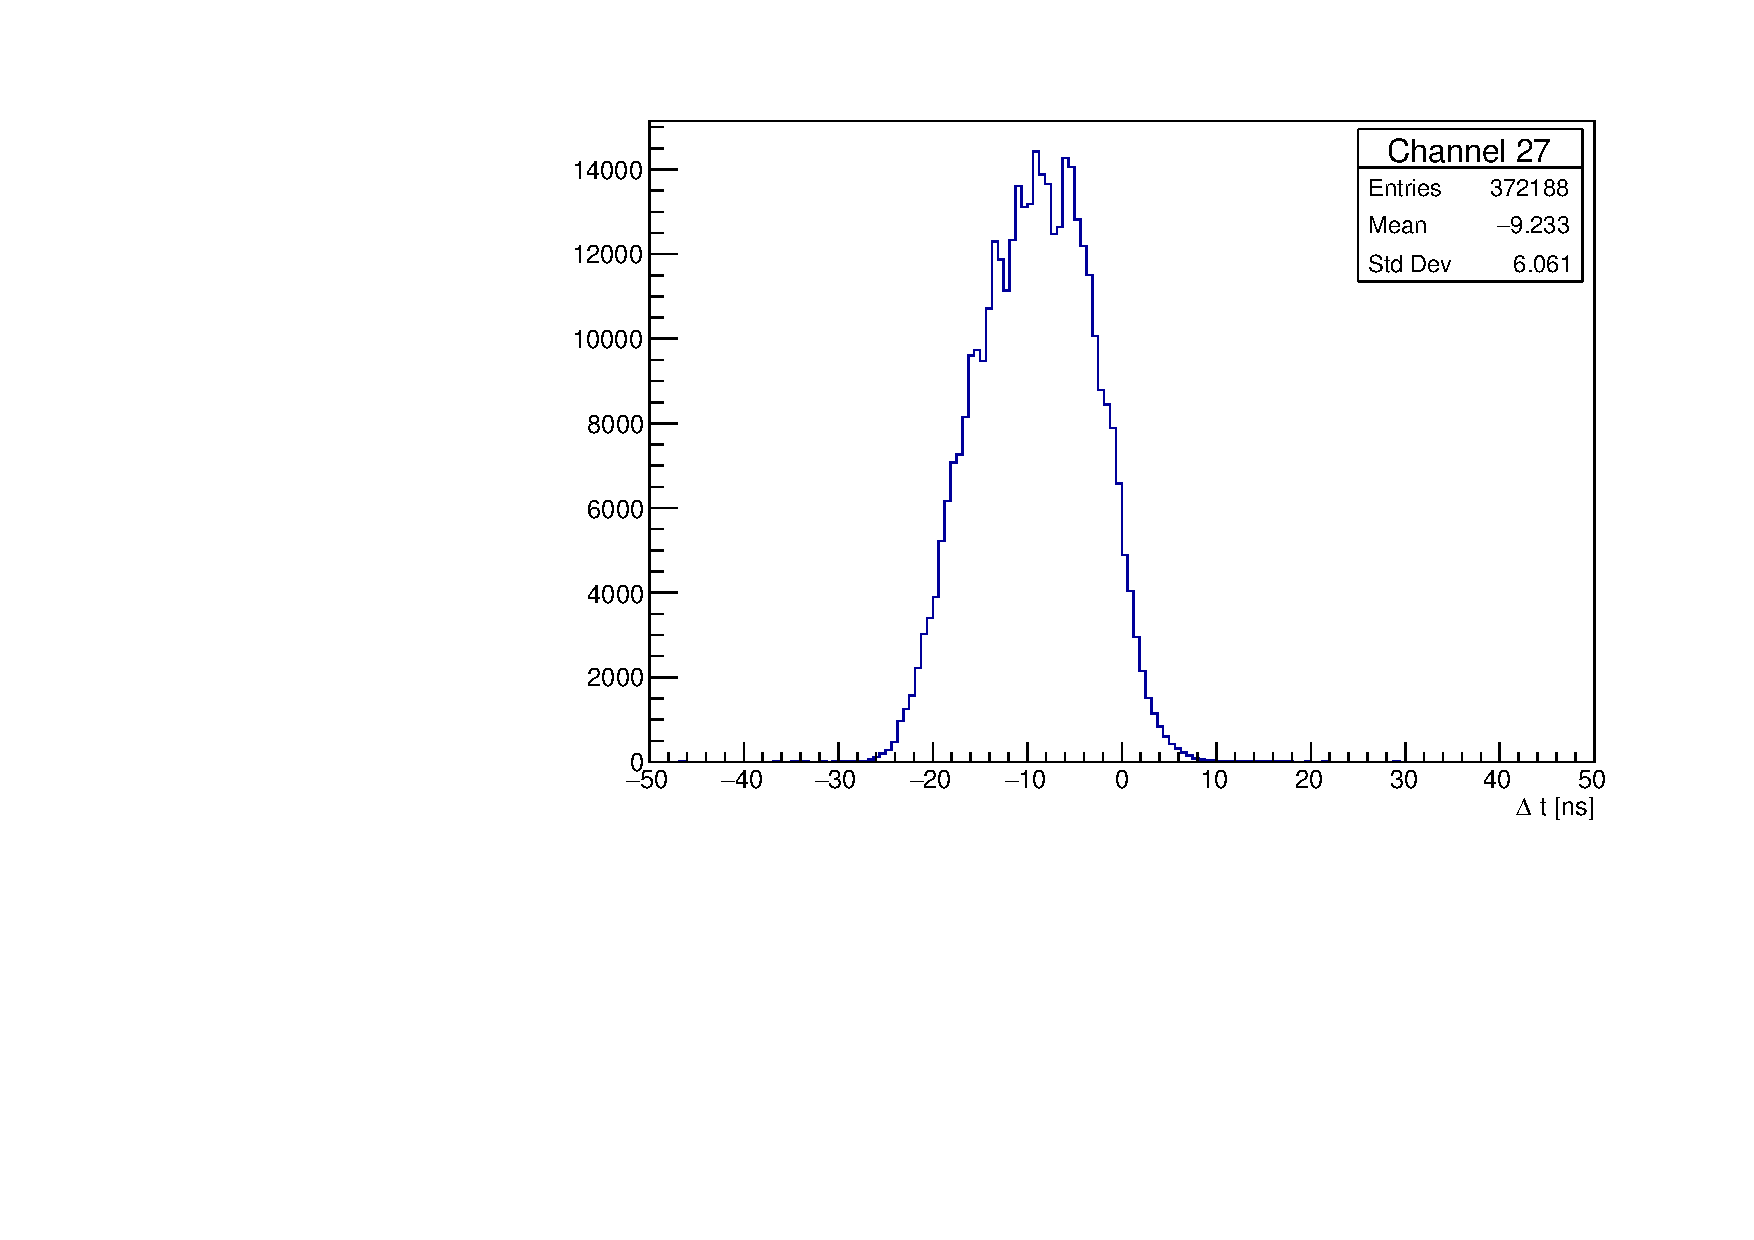
\includegraphics[width=0.49\textwidth]{figures/timingPlots/panels/Channel_27.pdf}
    \caption{\label{fig:timeDiffPanelLayer} Example time differences between panels and the closest layer. 
    The mean values are used to calibrate the panel timing.}
\end{figure}

The calibrations for each channel are summarised in table~\ref{tab:calibrations}. The 
standard deviation in the time difference between layers is $\sim5\unit{ns}$, allowing 
a time window of $15\unit{ns}$ to be defined for signal candidate events, as described in 
Section~\ref{sec:search}.

\begin{table}[ht!]
    \centering
    \scriptsize
    \topcaption{
	Time calibrations for each channel~\label{tab:calibrations}. The values are added to the raw time to define the calibrated time.
	}
	\begin{tabular}{ll}
	    Channel & Calibration (\unit{ns}) \\ 
	    \hline
	    0 &  33.125   \\
	    1 &  33.125  \\
	    2 &  13.75   \\ 
	    3 &  24.375  \\
	    4 &  23.75   \\
	    5 &  35.0    \\
	    6 &  30.625  \\
	    7 &  29.375  \\
	    8 &  24.375  \\
	    9 &  33.75   \\
	    10 & 3.75    \\
	    11 & 16.25   \\
	    12 & 26.875  \\  
	    13 & 34.375  \\
	    14 & 9.375   \\
	    15 & --     \\
	    16 & 27.5    \\
	    17 & 30.625  \\
	    18 & 0.0     \\
	    19 & 11.25   \\
	    20 & 7.5     \\
	    21 & 12.5    \\
	    22 & 28.125  \\
	    23 & 20.625  \\
	    24 & 33.75   \\
	    25 & 26.875  \\
	    26 & -3.125  \\
	    27 & 9.375   \\
	    28 & 13.75   \\
	    29 & 0.625   \\
	    30 & 15.625  \\
	    31 & 10.625     \\ 
	\end{tabular}
\end{table}

\section{Alignment}
\label{sec:alignment}

The alignment of the demonstrator is tested using muons originating from the proton-proton collisions 
at CMS (referred to as ``beam muons". Figure~\ref{fig:occ2d} shows the dependence of the total number of particles identified as having a muon pulse
in all four slabs on the luminosity of the LHC fill measured by CMS. There is a clear linear dependence with
a muon rate of $0.19/\pbinv$ measured in data, which agrees with the expected value from simulation
of a muon rate of $0.22/\pbinv$. This provides confidence the demonstrator is correctly aligned 
with the CMS interaction point.

\begin{figure}[ht!]
    \centering
    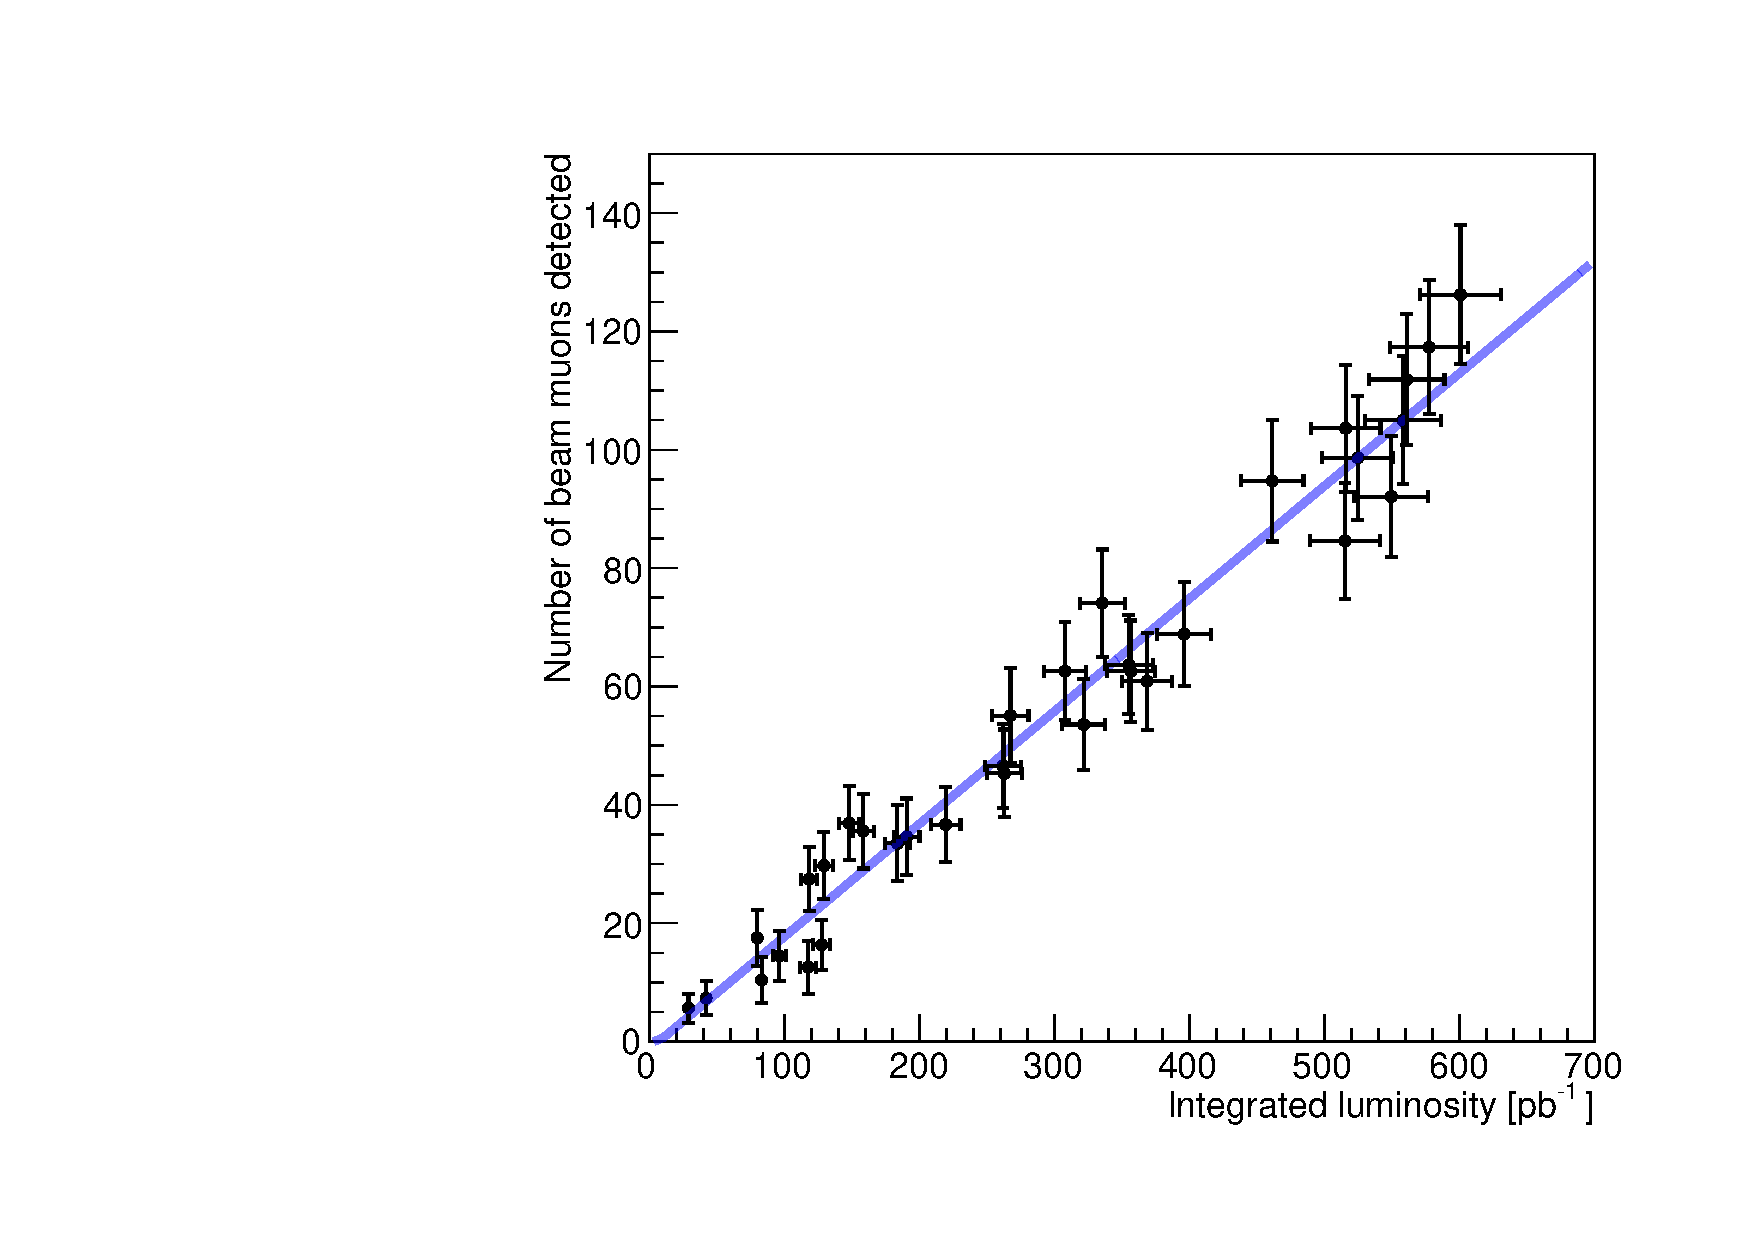
\includegraphics[width=0.6\textwidth]{figures/occ2d}
    \caption{\label{fig:occ2d} The occupancy of the milliQan demonstrator as a function of luminosity}
\end{figure}

The time difference between the slabs closest and furthest from the IP after the 
calibration described in Section~\ref{sec:timeCalibration} also provides confirmation
that the pulse timing can be used to discriminate between muons originating from the IP
travelling up through the detector and muons from cosmics travelling down through the detector. 
Figure~\ref{fig:timeDiff} shows well separated distributions from beam and cosmic muons with a time difference
consistent with that expected from the geometrical distance between the slabs ($2\times3.6/0.3 = 22\unit{ns}$).

\begin{figure}[ht!]
    \centering
    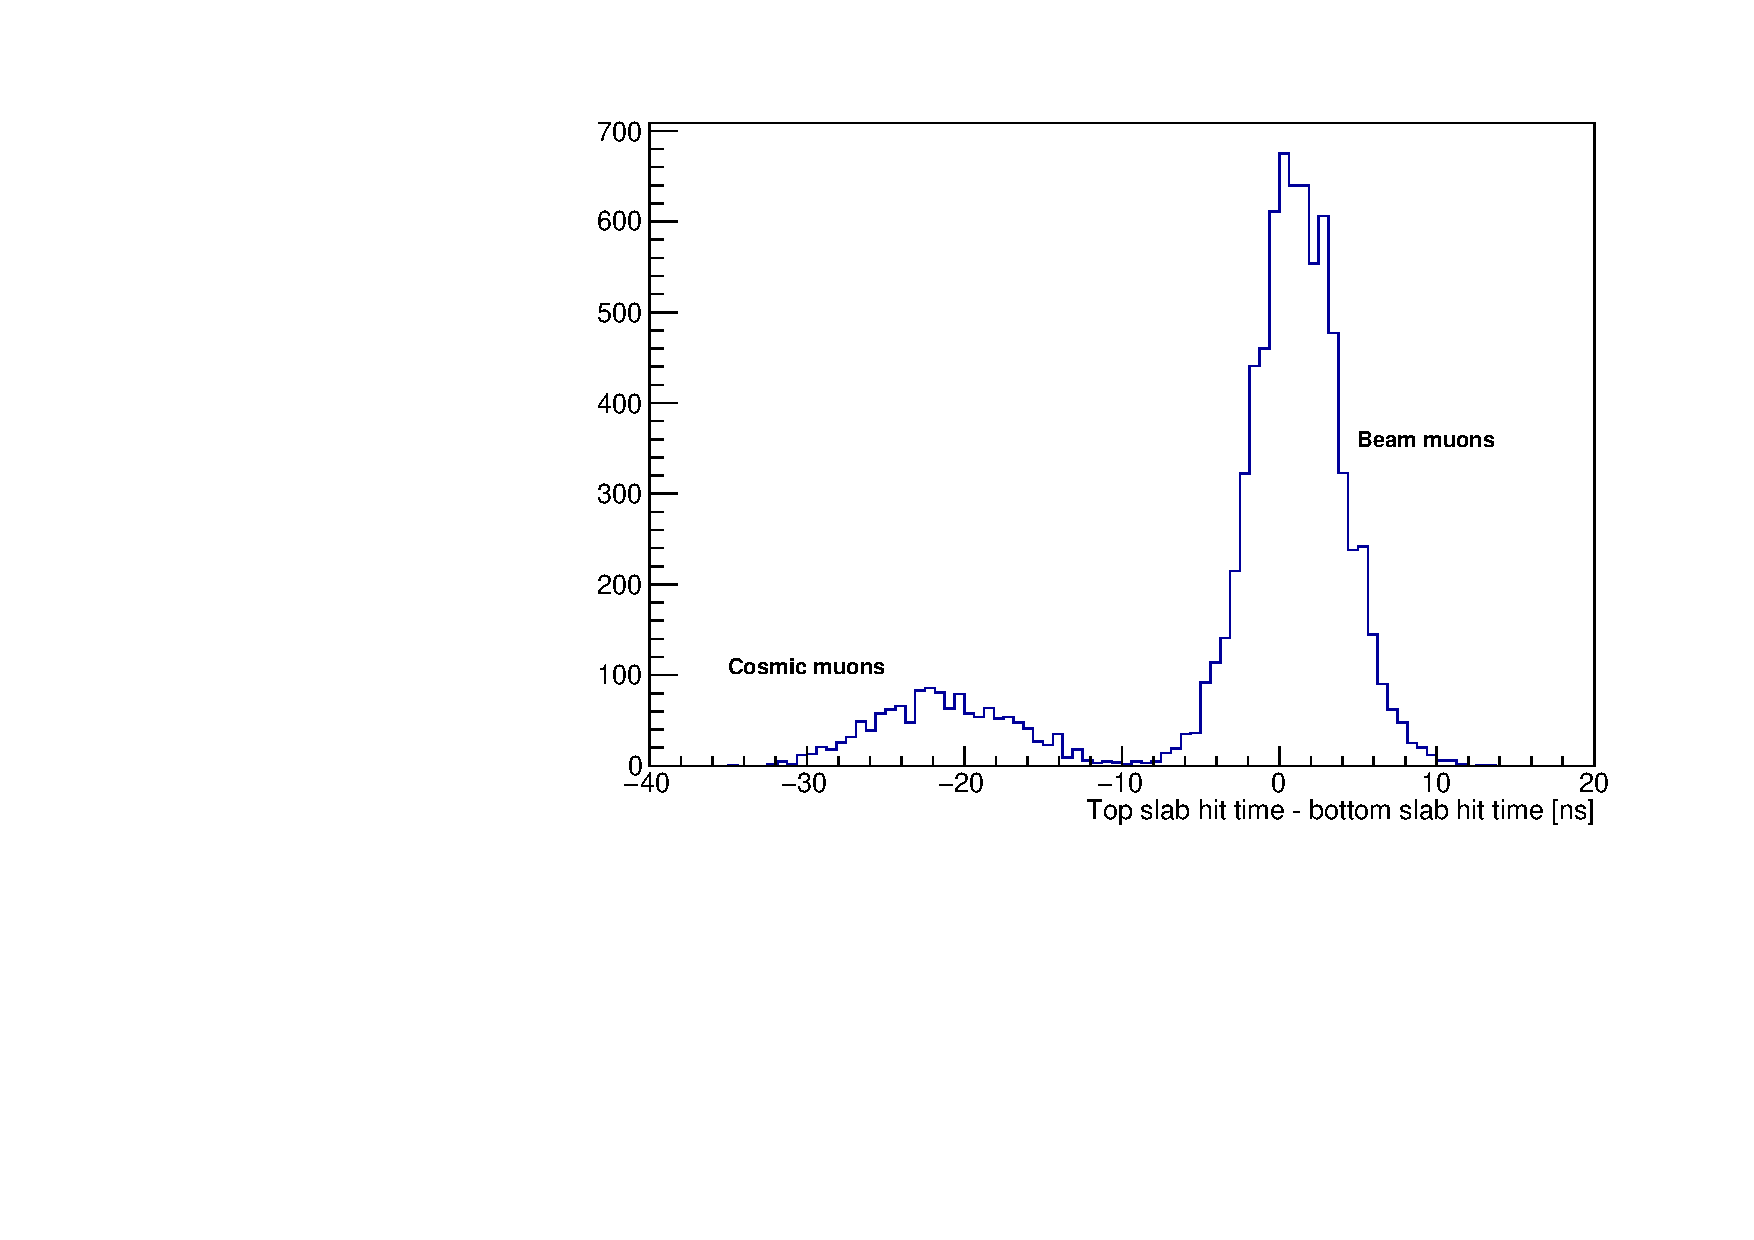
\includegraphics[width=0.6\textwidth]{figures/timeDiffSlabs}
    \caption{\label{fig:timeDiff} Time difference between the slabs furthest and closest to the CMS IP (channels 21 and 18 respectively).
    The peak at zero is consistent with originating from beam muons while the peak at $\sim -22\unit{ns}$ is consistent with originating from 
    cosmic muons.}
\end{figure}

\section{Search design}
\label{sec:search}

In this section a search for fractionally charged particles with the milliQan demonstrator is
detailed. The search relies on a triple coincidence of pulses across the three layers of the demonstrator. 
A range of selections are applied in order to reject contributions from
background sources, which are detailed below.

\begin{itemize}
    \item Dark rate overlap: each PMT has a dark current due to effects such as the thermal emission of electrons from the cathode. The simplest background source comes from random overlap of three such dark rate pulses. In addition, dark rate counts may overlap with a correlated double coincidence background from another source.
    \item Cosmic/beam muon showers: a large number of gammas, neutrons and electrons may be caused by an interaction of a cosmic ray muon with the rock in the demonstrator cavern. This may cause a pulse in each layer of the milliqan demonstrator. Such a background could also be expected from a beam muon which travels close to the demonstrator.
    \item Radiation: radiation in the cavern, scintillator bars or surrounding material can cause correlated deposits in several bars. The lead blocks placed between layers should reduce the probability of a three layer deposit arising from photons or electrons, however, neutrons will not be shielded. 
    \item Afterpulses: afterpulses arising from correlated deposits may overlap and produce a triple coincidence signature in the demonstrator. The original correlated signature must not be triggered as in this case the afterpulses will fall in the readout deadtime and not be recorded.
\end{itemize}

Each event is required to have a pulse in
a single bar in each layer in order to pass signal selection. If there is activity in any slab or panel the event is 
vetoed. These requirements reject backgrounds due to cosmic showers, which are expected to cause deposits
across the detector and beam muons passing close to the bars, which will cause significant pulses in
the slabs. The bars which contain hits are additionally required to be pointing to the IP such that they 
have the same position which each layer. This reduces the background from neutrons, cosmic showers and random overlap
while being efficient for signal which is expected to have a small angular spread. In each bar a requirement is
made of exactly one pulse and low sideband activity to reject backgrounds from overlapping afterpulses. Finally, the
maximal calibrated time difference between pulses in different bars is required to be less than 15\unit{ns}, which is 
efficient for signals travelling upwards from the IP and forms a powerful rejection of backgrounds
with different paths through the detector or that have deposits 
in each layer that are uncorrelated in their timing.


\section{Background determination}

The total background as a function of the minimal \npe in the event can be evaluated 
using data taking periods in which there are no collisions and scaled to the 
total length of the data taking with collisions. This is shown in Figure~\ref{fig:bkgNoBeam}.
The background ranges from 122 events for $0.5 < \npe < 1.5$ values to 2.6 events for $\npe > 10$.

\begin{figure}[ht!]
    \centering
    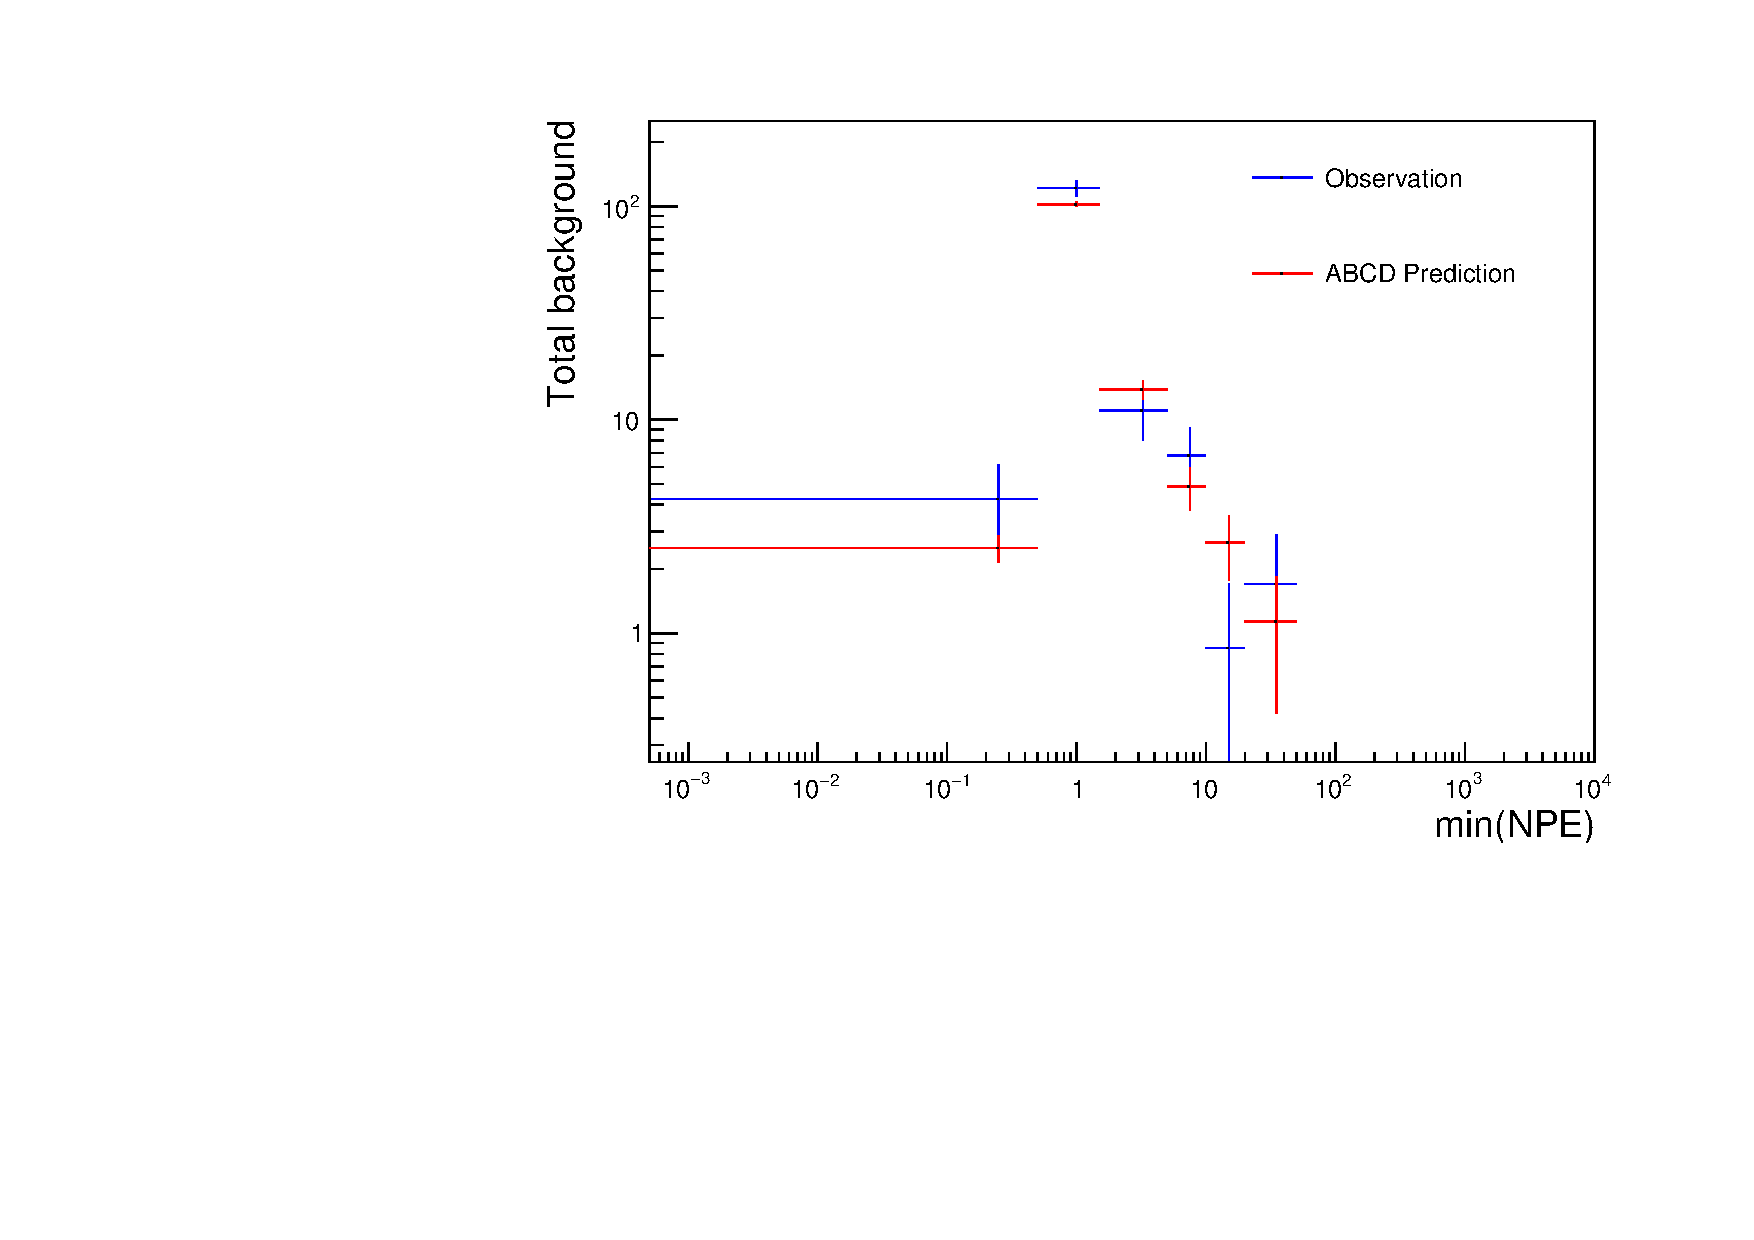
\includegraphics[width=0.6\textwidth]{figures/backgroundYieldsNoBeam_15ns_07}
    \caption{\label{fig:bkgNoBeam} The minimal \npe in the event during data-taking period with 
    no collisions for events passing the signal selection is
   compared to the prediction from the ABCD method detailed in the text.}
\end{figure}

\begin{figure}[ht!]
    \centering
    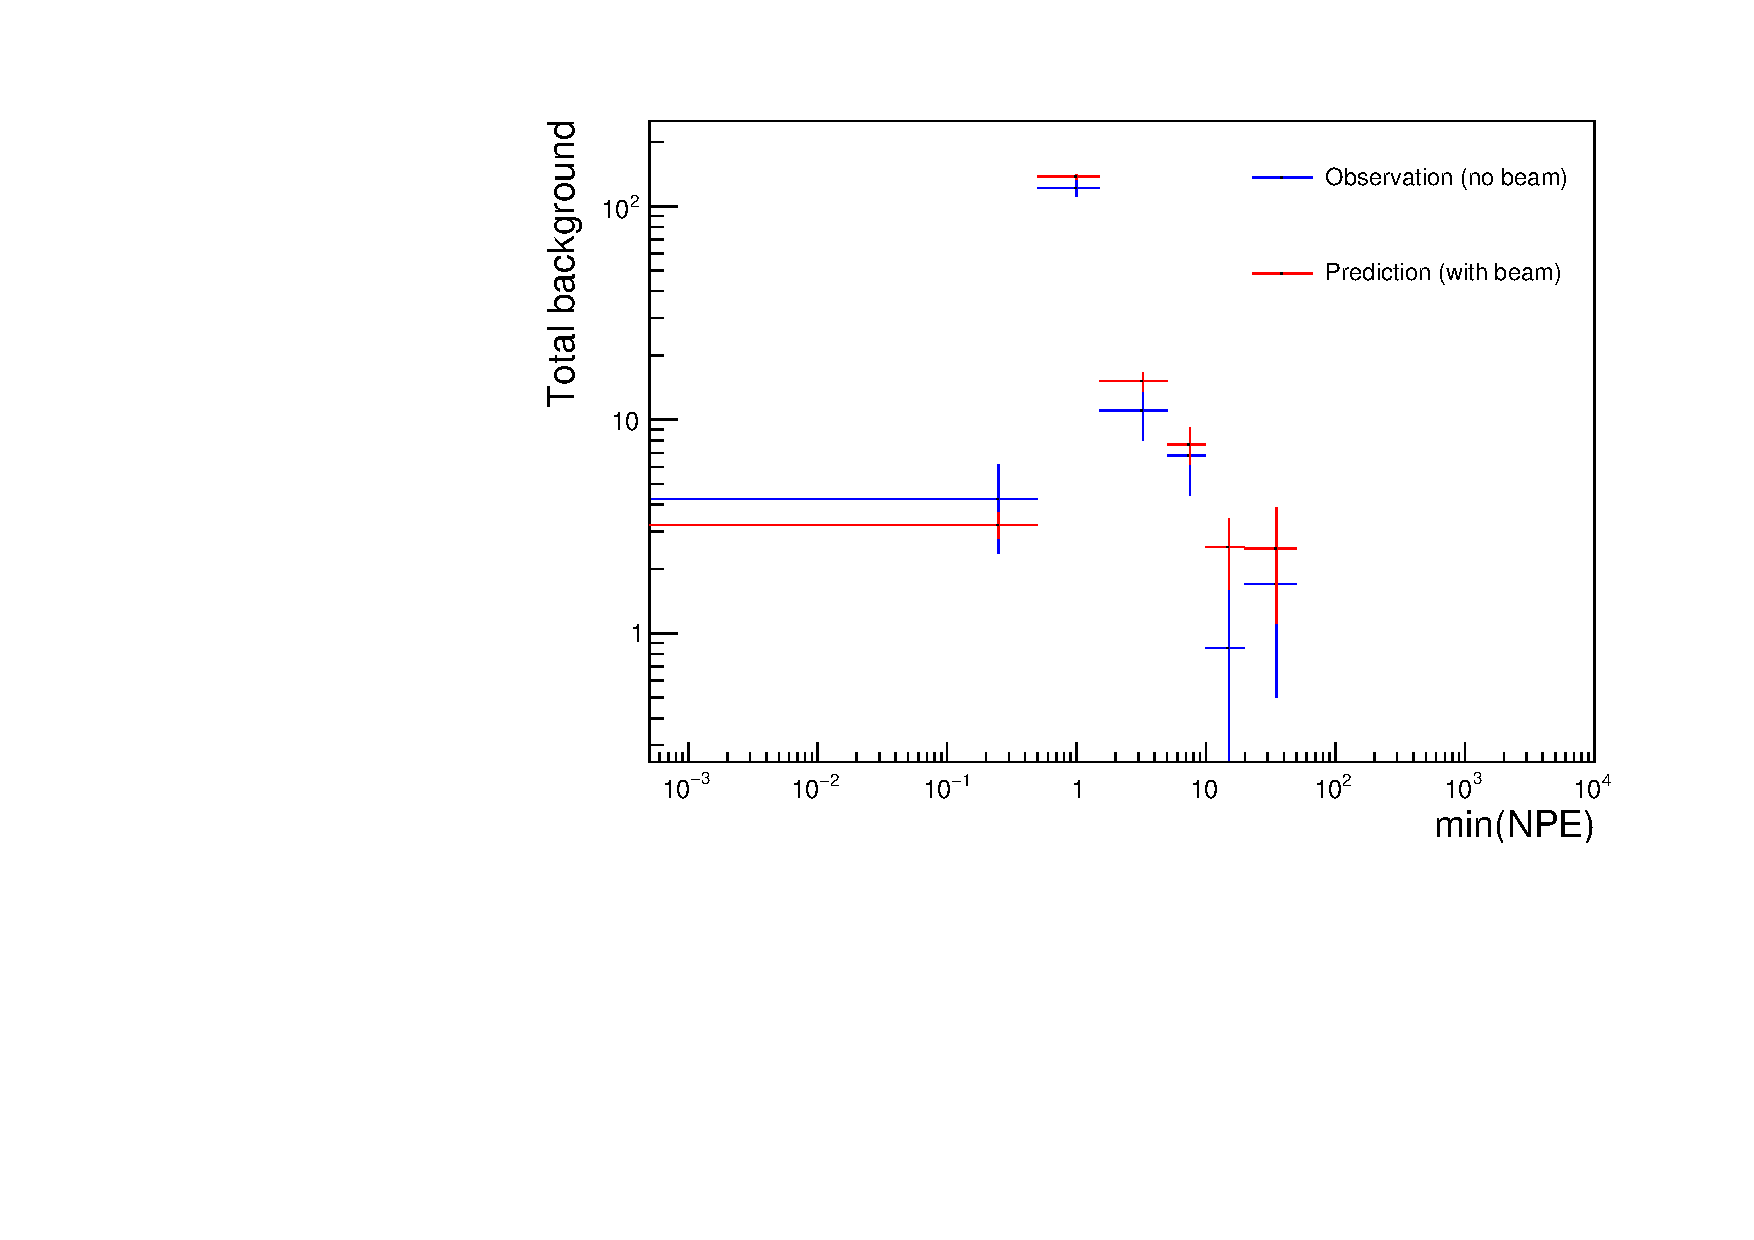
\includegraphics[width=0.6\textwidth]{figures/backgroundYieldsWithBeam_15ns_07}
    \caption{\label{fig:bkgWithBeam} The minimal \npe in the event during data-taking period with 
    collisions for events passing the signal selection is
    compared to the prediction from the ABCD method detailed in the text.}
\end{figure}

In order to validate there are no additional backgrounds introduced from collisions, signal depleted
control regions are defined by inverting the maximal time difference and pointing path requirements.
The background in the signal region is then predicted using the ABCD method for each region
in \npe, where the prediction follows $N_A = N_B\times N_D/N_C$ and the regions are defined in Table~\ref{tab:ABCDregions}. 
This prediction is carried out for both the data taking periods with and without collisions and compared
to the observation in the data taking period without collisions, as shown in Figures~\ref{fig:bkgNoBeam} 
and~\ref{fig:bkgWithBeam}, respectively. Both predictions are seen to agree well with the observation, 
validating the use of data taken during periods without collisions to measure the background.

\begin{table}
    \centering
    \scriptsize
    \topcaption{The region definition for the ABCD prediction.\label{tab:ABCDregions}}
    \begin{tabular}{lll}
	Region& Time selection & Path selection\\
	A (signal) & $\text{max}(\Delta t) < 30 \unit{ns}$ & Pointing path\\
	B & $\text{max}(\Delta t) > 30 \unit{ns} \text{ and } \text{max}(\Delta t) < 100 \unit{ns}$ & Pointing path\\
	C & $\text{max}(\Delta t) > 30 \unit{ns} \text{ and } \text{max}(\Delta t) < 100 \unit{ns}$ & Non-pointing path\\
	D &$\text{max}(\Delta t) < 30\unit{ns}$ & Non-pointing path\\
    \end{tabular}
\end{table}

In order to determine the sources of the background observed in the signal region 
various studies have been carried out and are documented in the remainder of this section.

\subsection{Dark rate overlap background}

The first background source that was considered is the dark rate overlap. The dark rate is measured
for each channel using ``zero bias" runs in which the data is collected with a random trigger.
The average dark rate for the bars is shown in Figure~\ref{fig:darkRate}. This can be used to estimate the 
contribution from the random overlap of three dark counts in three bars. 
The prediction as a function of \npe is shown in Figure~\ref{fig:ratePred} and 
compared to the observation in the signal region during data taking periods without collisions. 
Random overlap of dark rate can be seen to account for $\sim25\%$ and $\sim0.4\%$ 
of the overall rate for \npe values of $\sim 1$ and $> 5$, respectively. The dark rates are 
known to vary with time and so this prediction should be repeated with a time
dependent measurement.

Finally, the background per path is shown in Figure~\ref{fig:perPathPlot}. The paths involving
the channels with the highest dark rates are seen to have the highest 
significantly higher triple coincidence rate for \npe < 5. For \npe > 5 the
rate is comparable for all paths.
\begin{figure}[ht!]
    \centering
    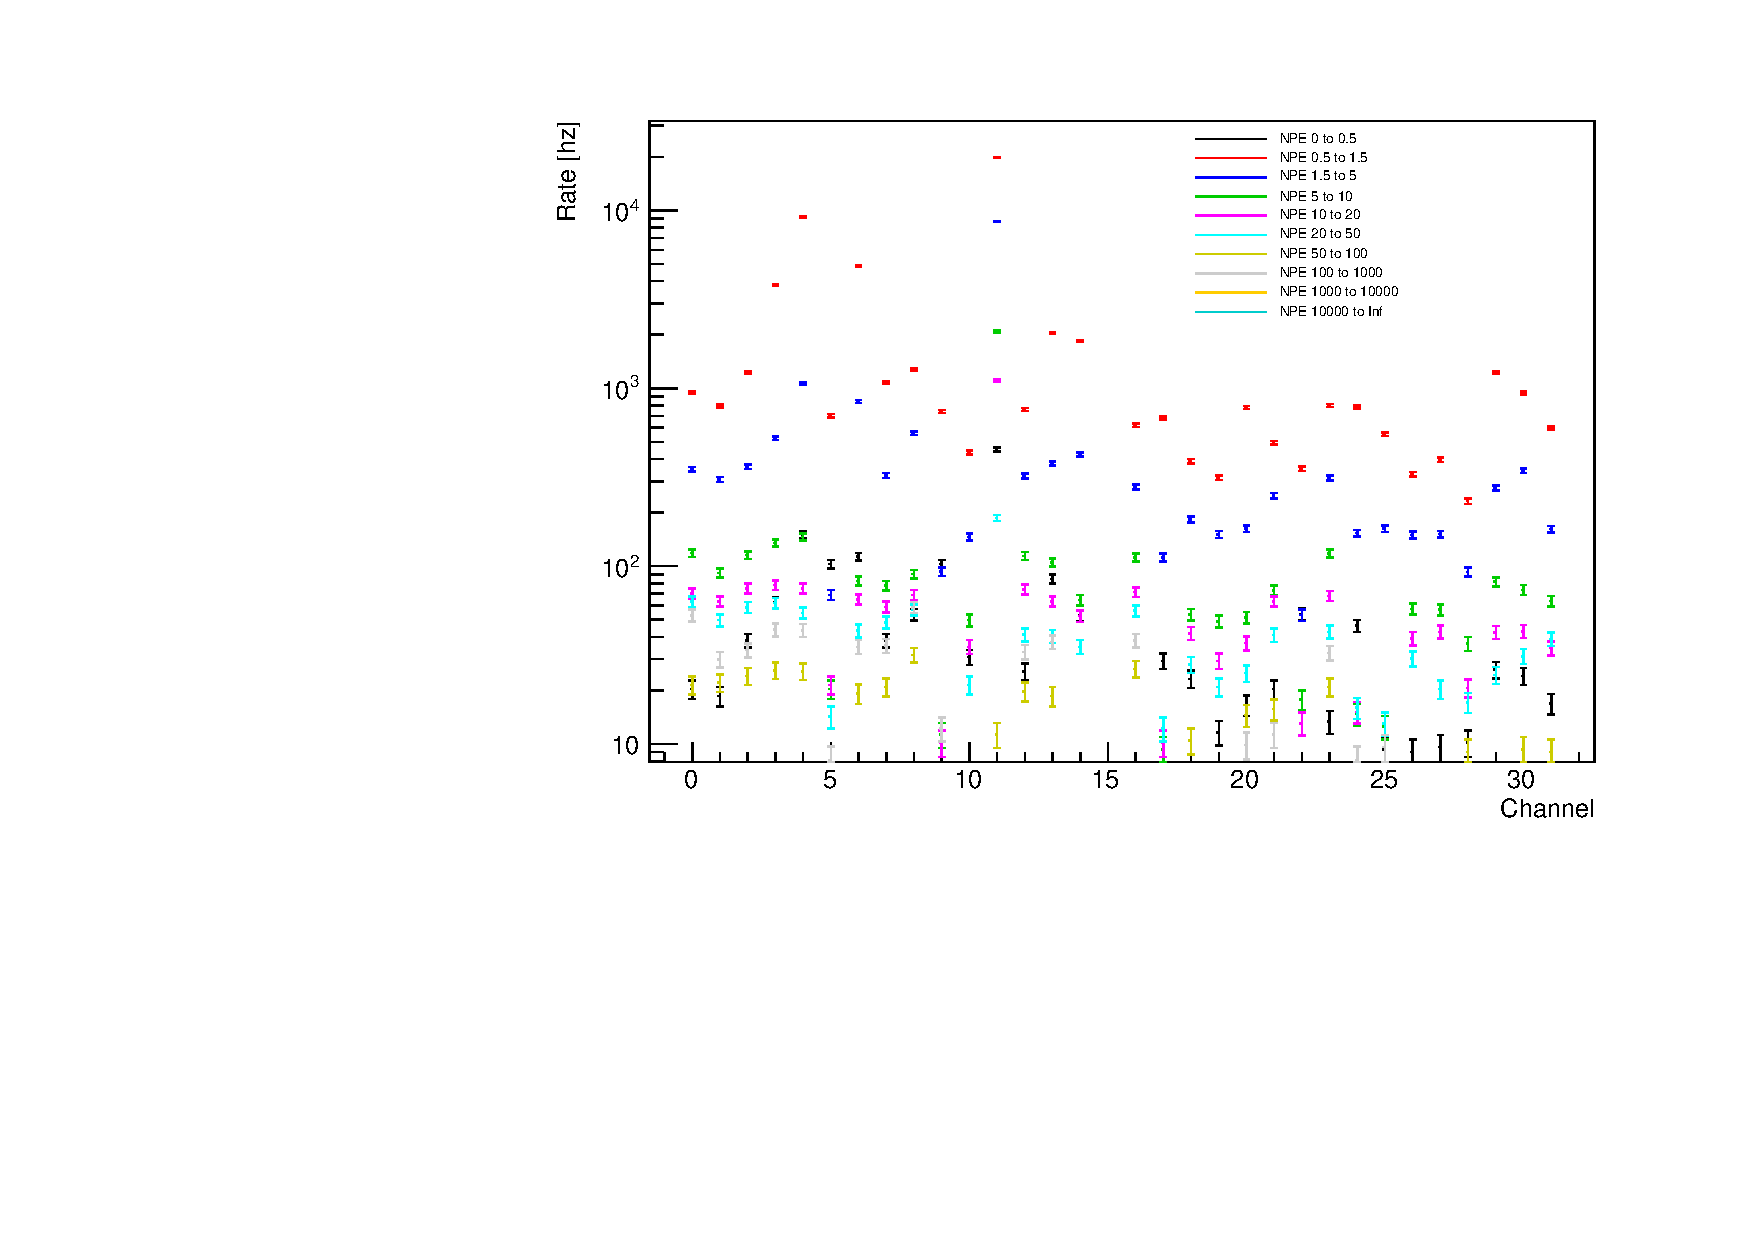
\includegraphics[width=0.6\textwidth]{figures/singlesRatesUnbiasedQuietSinglePulseInChanHeightAllUnbiasedBinnedAsSignal}
    \caption{\label{fig:darkRate} Single channel rate for an inclusive \npe selection measured using zero bias runs.}
\end{figure}

\begin{figure}[ht!]
    \centering
    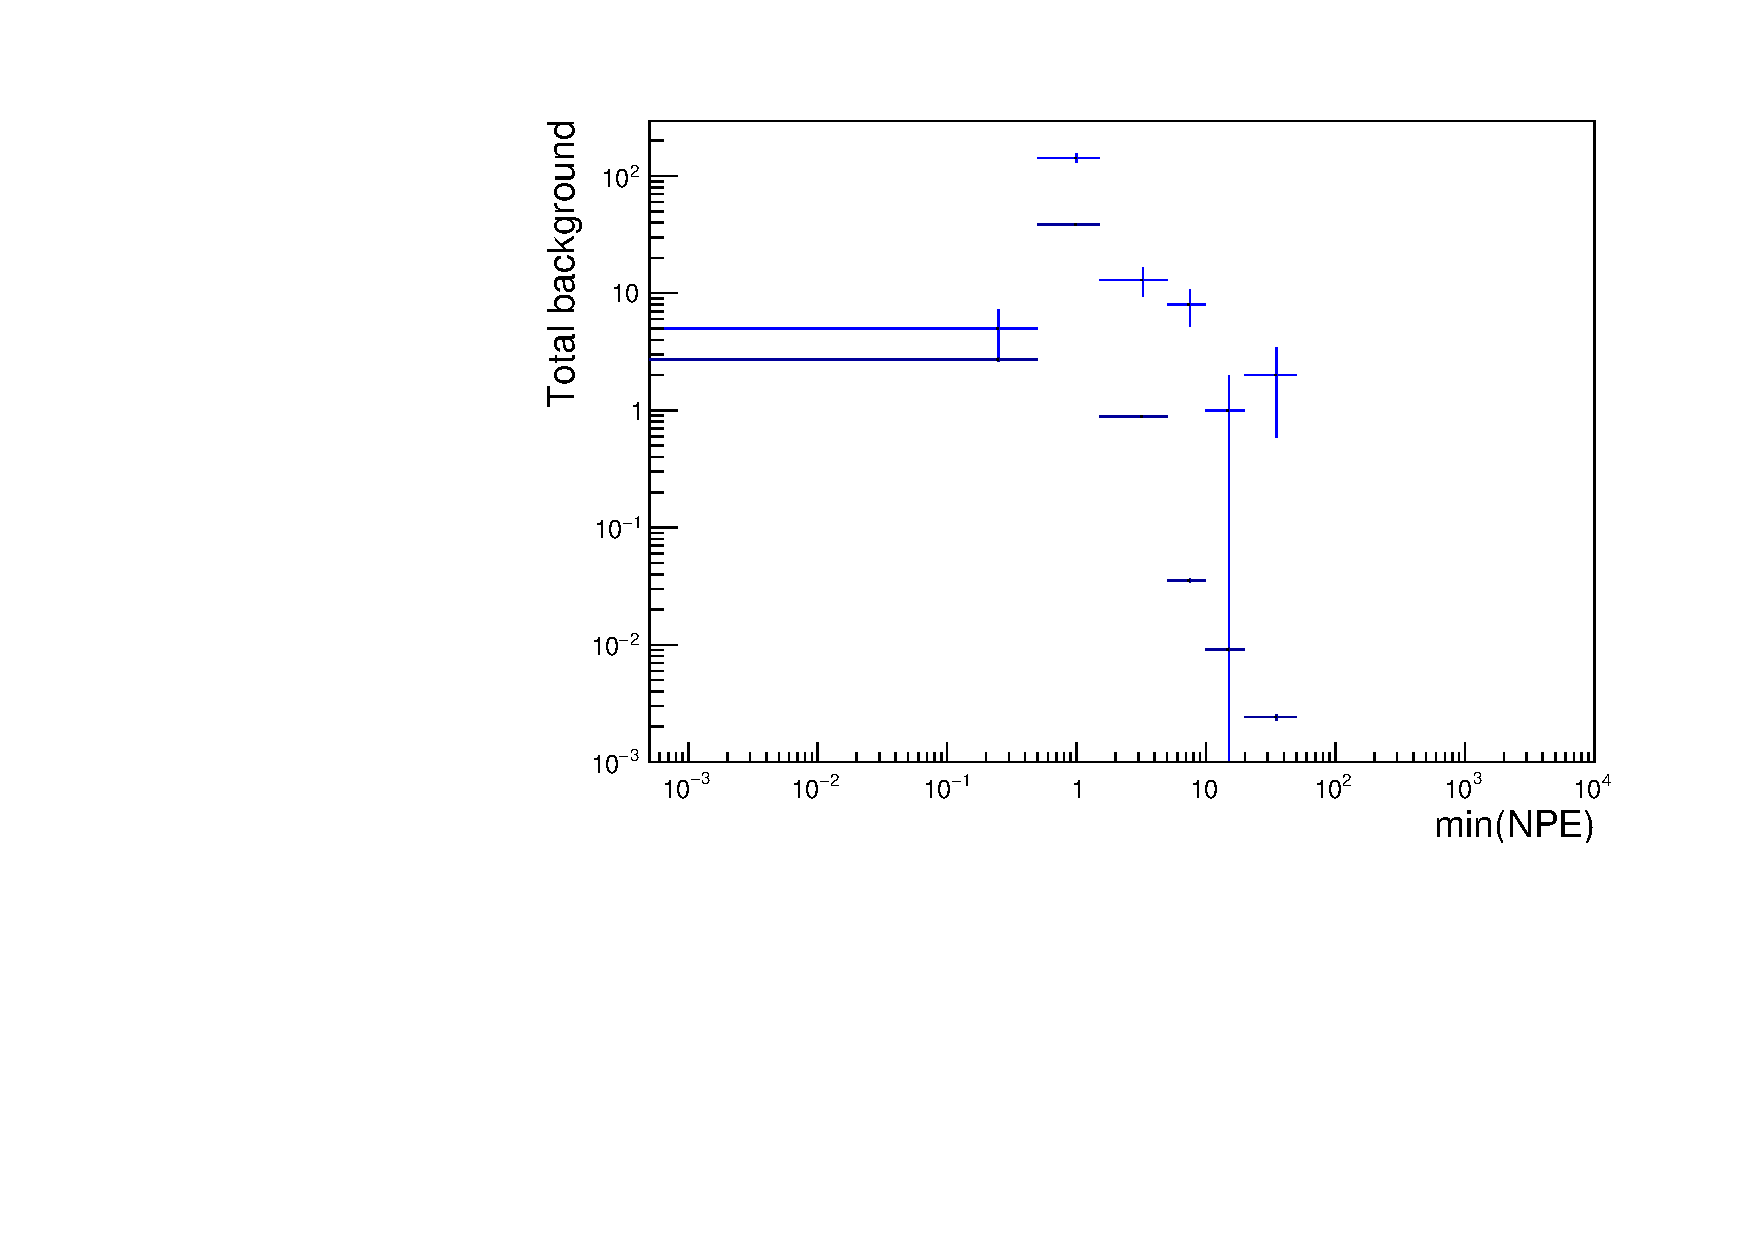
\includegraphics[width=0.6\textwidth]{figures/predictionAndMeasurementTimeWindow15}
    \caption{\label{fig:darkRate} Background predictions for a signal like selection
    from dark rate is compared to the observation in the data taking period without beam.} 
\end{figure}

%FIXME - this rate is seen to vary with time, evaluate this dependence for single channel and 
% triple coincidence in the signal region!

\begin{figure}[ht!]
    \centering
    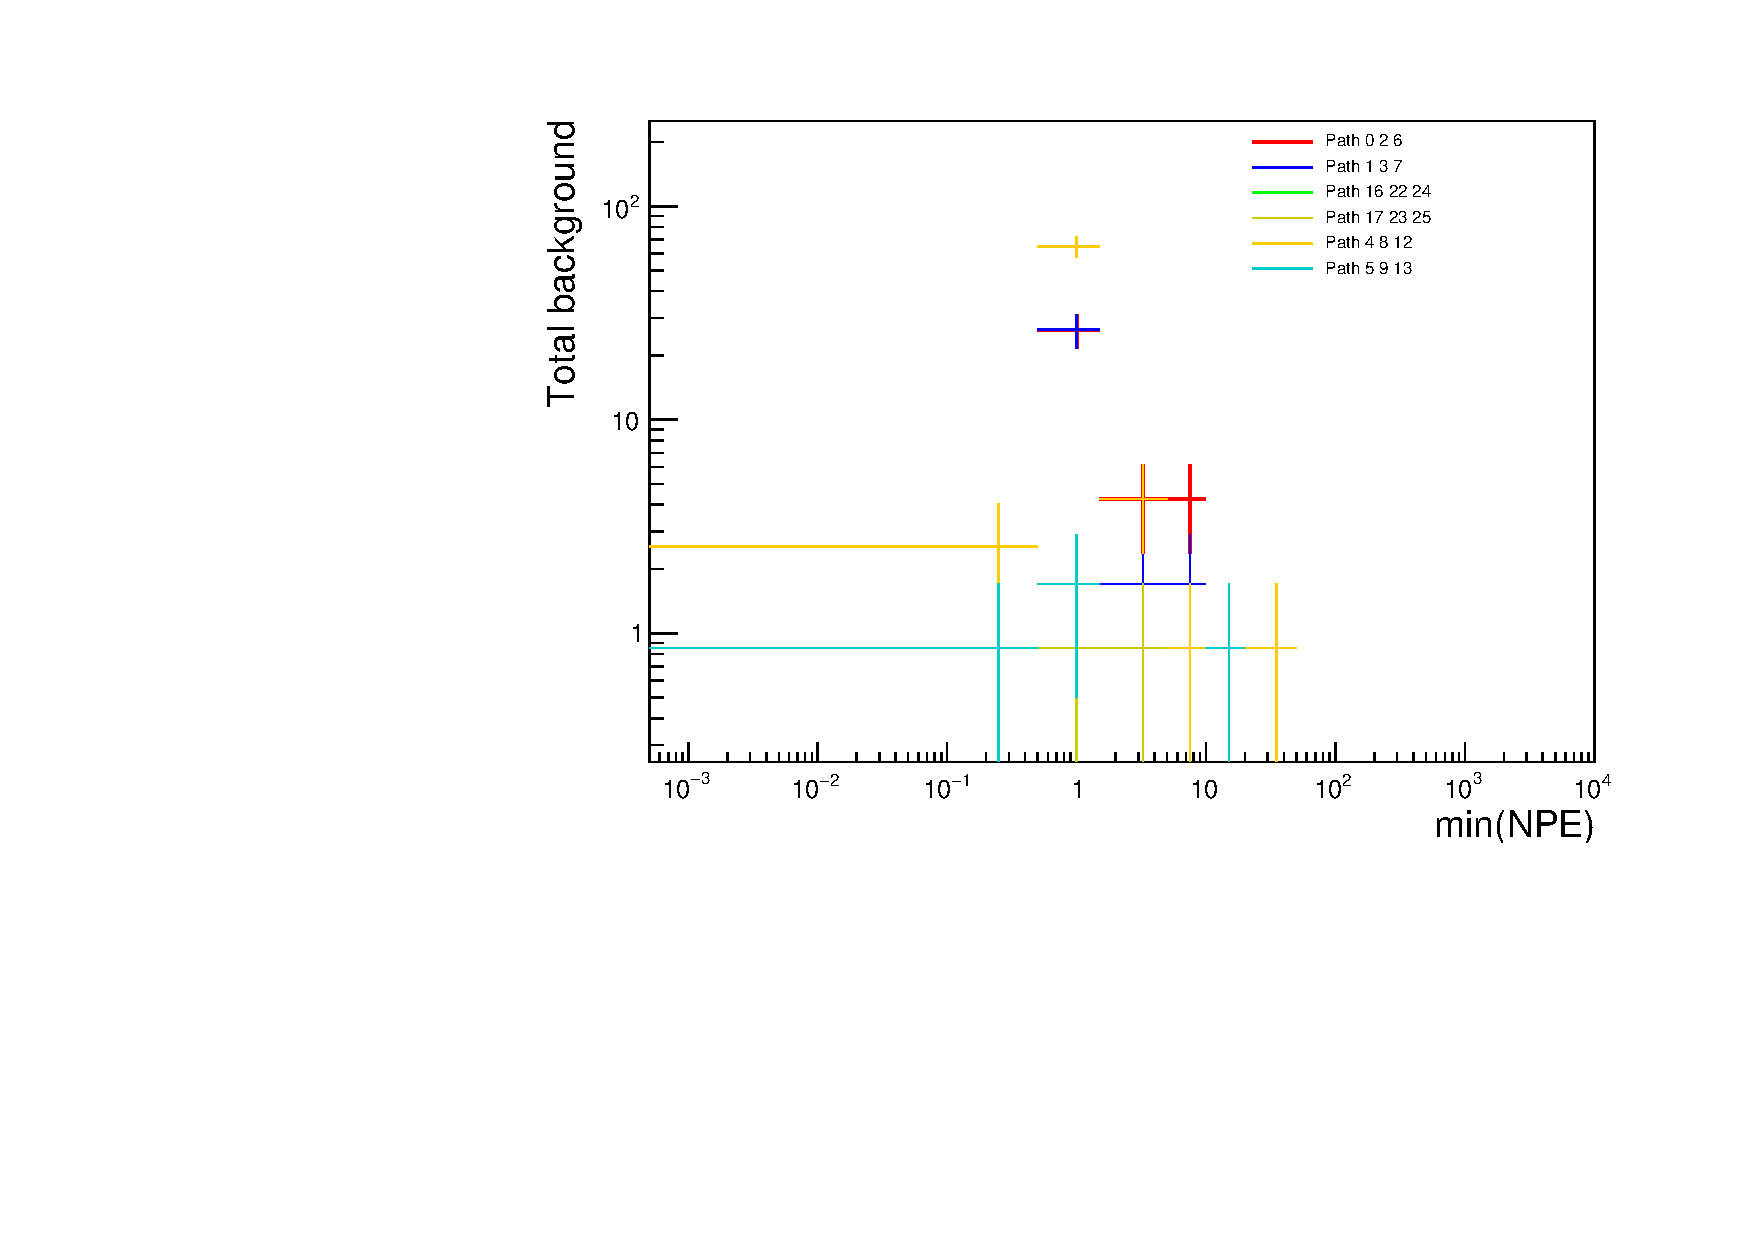
\includegraphics[width=0.6\textwidth]{figures/perPathPlotsNoBeam.pdf}
    \caption{\label{fig:perPathPlot} The minimal \npe in the event during data-taking period without
    collisions for events passing the signal selection is shown for each pointing path 
    through the demonstrator.}
\end{figure}

\subsection{Radiation}

To be filled ...

\subsection{Cosmic/beam muon showers}

To be filled ...

\subsection{Afterpulses}

To be filled ...

\section{Interpretation}

Signal efficiencies from injection tests and prototype interpretations
\section{Summary}

The alignment and calibration of the milliQan demonstrator have been detailed. The calibrated
data have been used to search for fractionally charged particles with new 
exclusion sensitivity expected for masses between $\sim0.1$ and 5\unit{GeV} 
and charges between $\sim0.02$ and $0.1e$.

\appendix
\section{LED bench studies}
\label{app:speLEDCalib}
In this appendix the studies undertaken using PMTs coupled to an LED source are documented.
The experimental setup is shown in Figure~\ref{fig:LEDSetup}. The LED is a Thorlabs LED430L with a 430\unit{nm} wavelength 
and representative R878, R7725 and ET PMTs are studied. The DRS scope is triggered on
the LED pulse meaning the PMT response falls in a well-defined time window 
and removing the need for pulse finding. The pulse areas for a range of R878 HVs are
shown in Figure~\ref{fig:LEDPulseAreas}. The average \npe input to the PMT can be controlled by varying the amplitude of the input LED pulse.
This setup was used to study the SPE area, afterpulses and create an SPE template for 
pulse and signal injection tests. 

\begin{figure}[ht!]
    \centering
    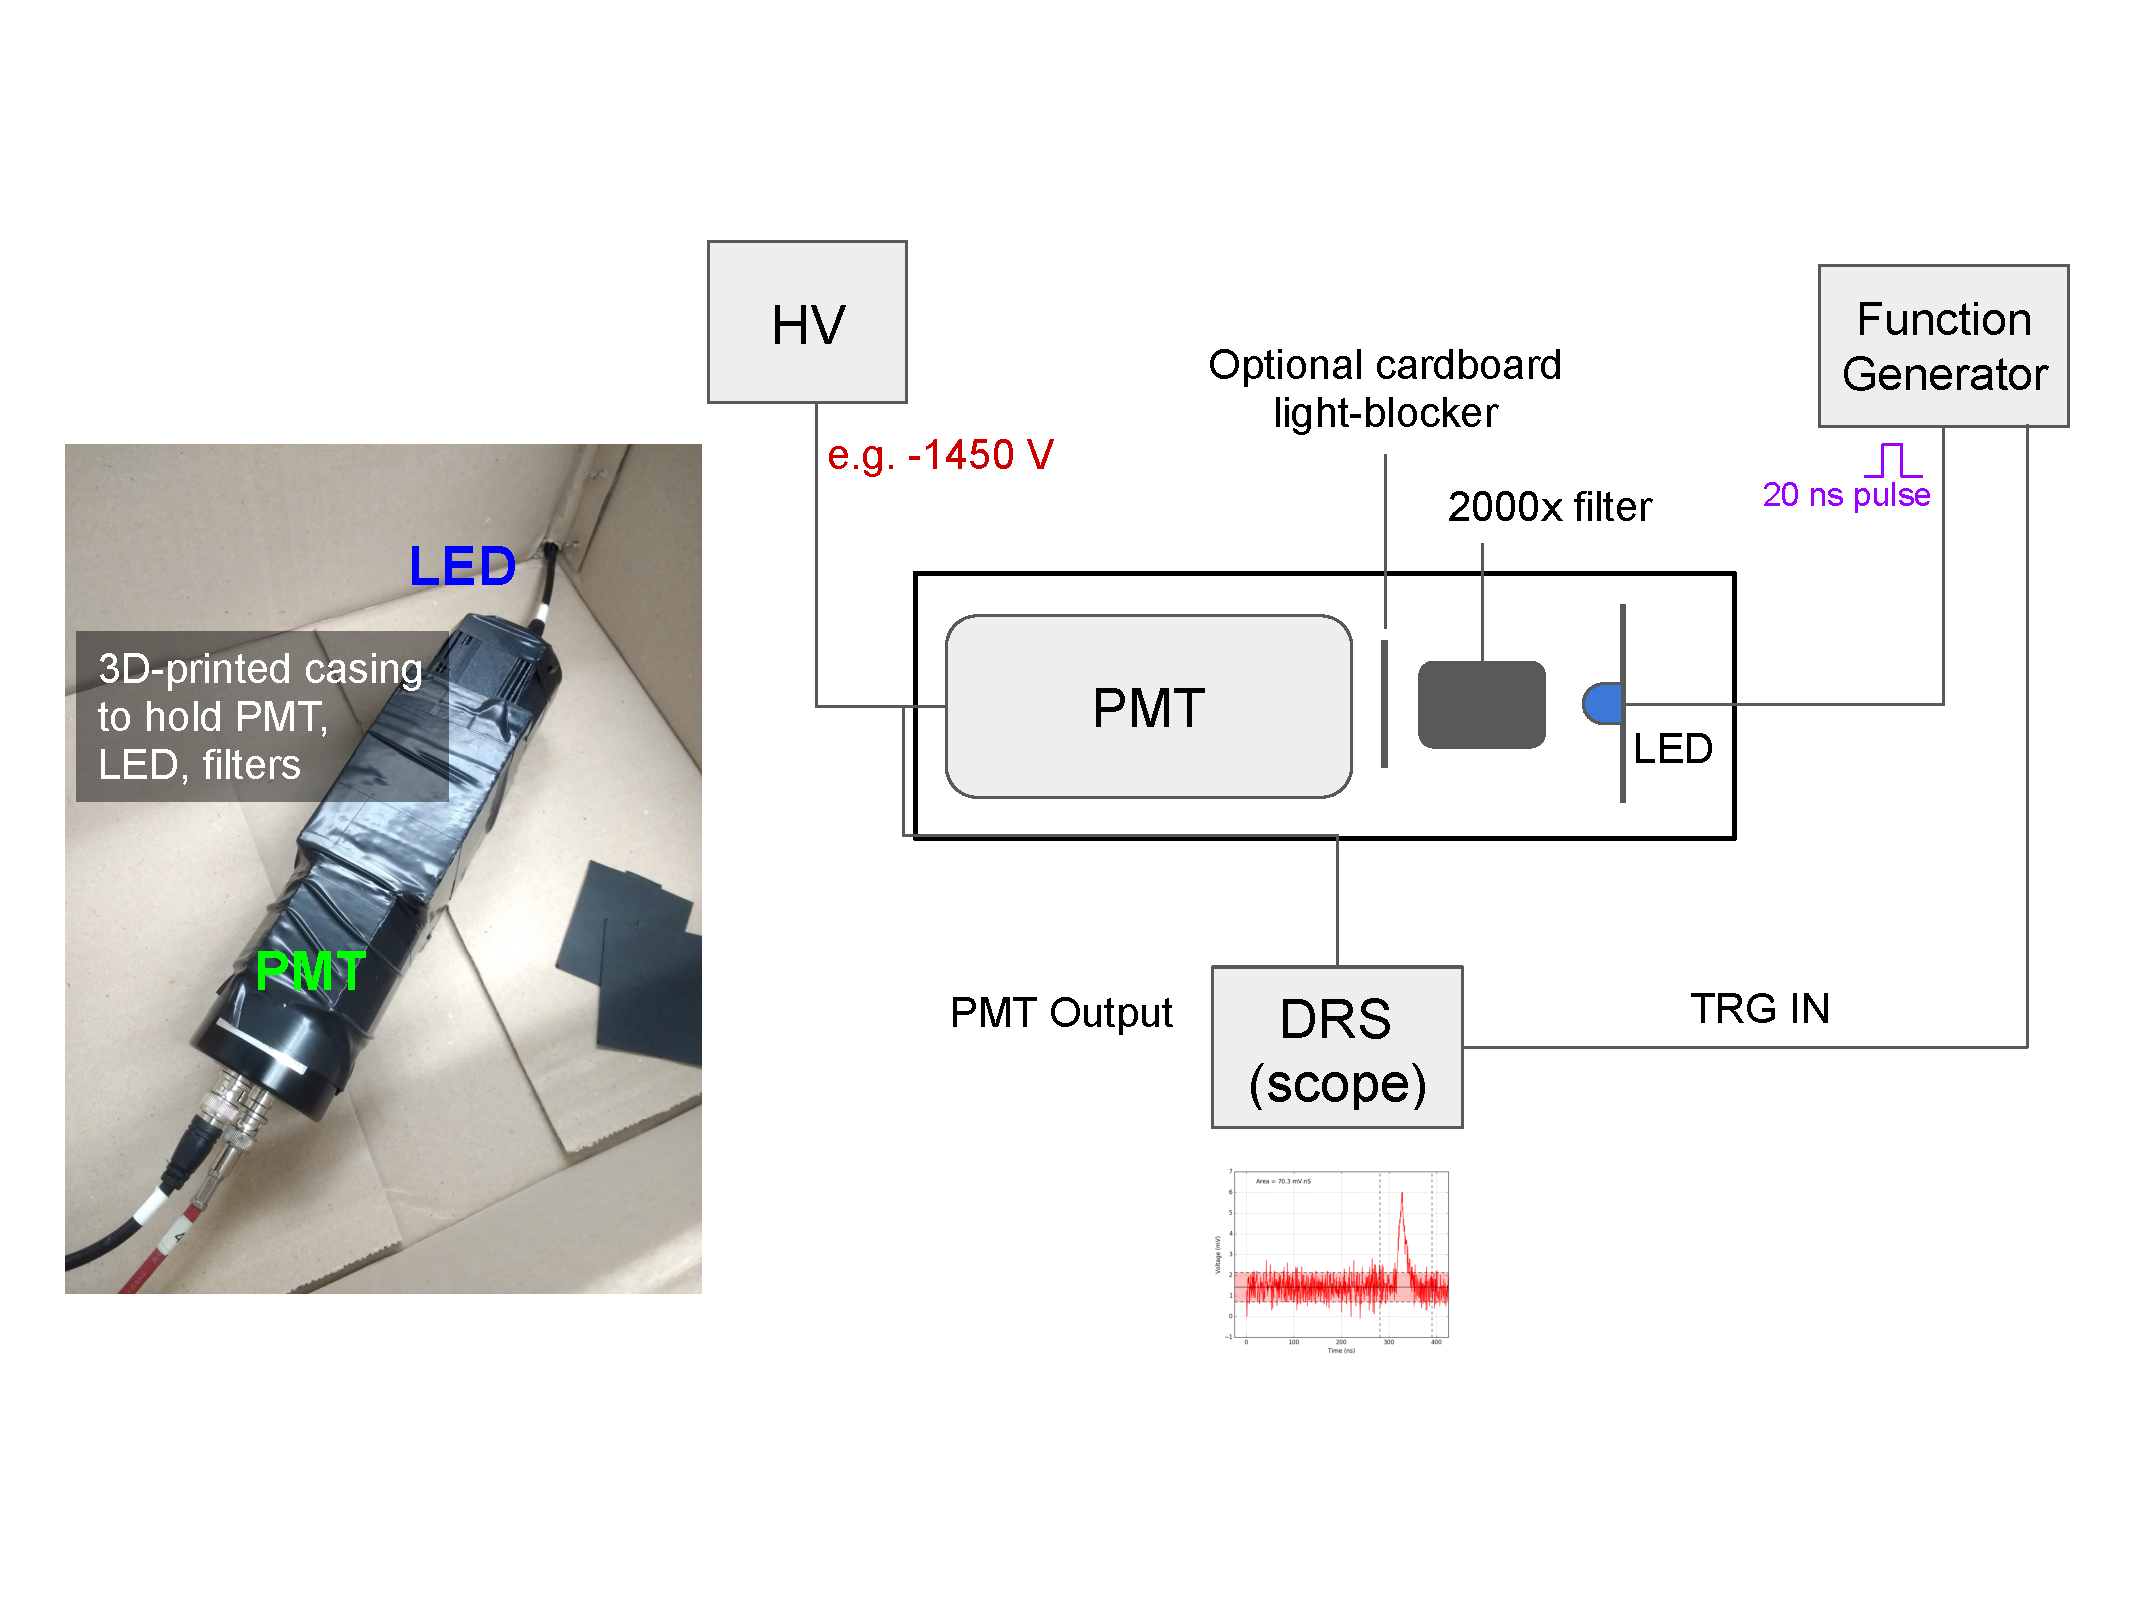
\includegraphics[width=0.8\textwidth]{figures/LEDsetup}
    \caption{\label{fig:LEDSetup} The experimental setup used for the LED bench studies. }
\end{figure}


\begin{figure}[ht!]
    \centering
    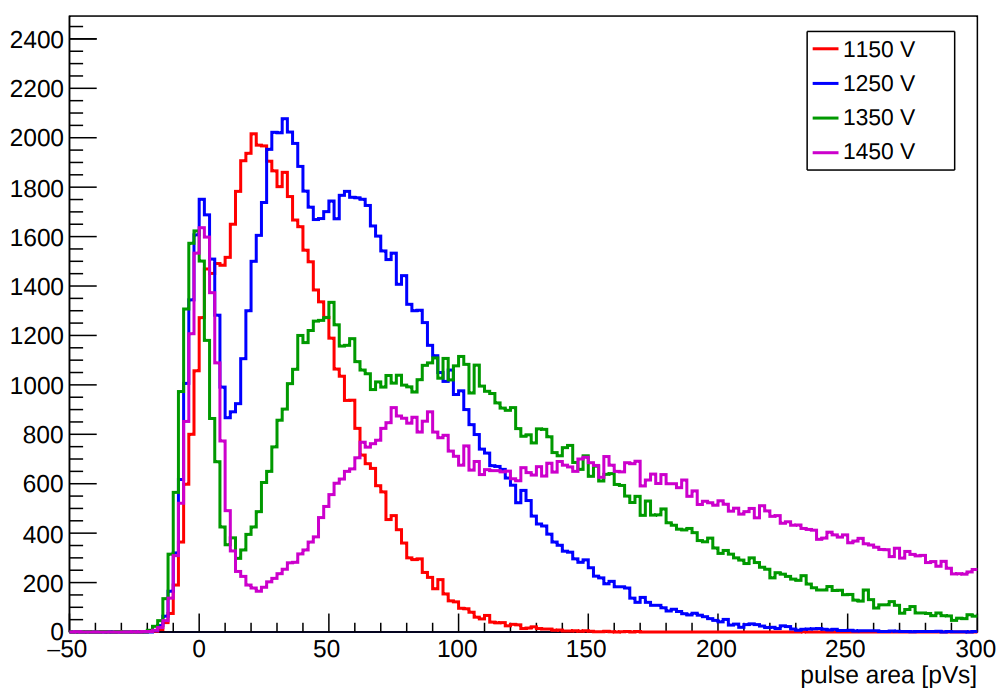
\includegraphics[width=0.8\textwidth]{figures/LEDareas}
    \caption{\label{fig:LEDPulseAreas} The area distributions for several R878 PMT HVs. The peaks correspond 
    to 0, 1 and 2 SPEs and their separation increases with HV.}
\end{figure}

\subsection{SPE area measurement}
\label{sec:ledarea}
The calibration of the SPE area using an LED allows the impact of "partial" SPE pulses to be considered.
Such pulses can occur in the PMT due to non-optimal trajectories such as the photon passing through the cathode and directly
striking the first dynode or a PE skipping a dynode. The calibration procedure follows the method described
in Ref.~\cite{Saldanha:2016mkn}. First, the zero SPE pulse area distribution is measured by taking data with the LED blocked.
Next, the pulse area distribution is measured with the LED on and the zero SPE distribution scaled to match the left edge of 
this distribution. This is shown in Figure~\ref{fig:SPEcalib}. The fraction of zero SPE events to be estimated and, assuming 
a Poisson distribution, the average \npe from the LED can be calculated as $\left< \npe \right> = -\log(f)$.

\begin{figure}[ht!]
    \centering
    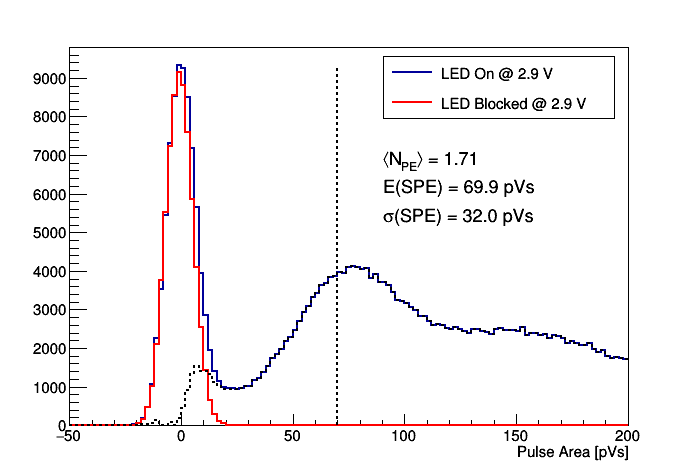
\includegraphics[width=0.8\textwidth]{figures/speCalib}
    \caption{\label{fig:SPEcalib} The pulse area distributions used to calibrate the SPE area for
    $\text{HV}=1450\unit{V}$.}
\end{figure}

The average SPE area can then be trivially calculated as 
$\left<\text{area}_\text{on}\right>-\left<\text{area}_\text{blocked}\right>/\left<\npe\right>$.
The result of this procedure is shown in Figure~\ref{fig:r878calib} for a range of HV values. 
The measured value for 1450\unit{V} is in good agreement with the 
in-situ measurement of the R878s described in Section~\ref{sec:npeCalibration}.

The measurement of the SPE area for an R7725 and an ET PMT 
is shown in Figure~\ref{fig:r7725calib} and~\ref{fig:etcalib} respectively.
In the case of the R7725 the SPE area is significantly larger compared to the R878 and
has a larger proportion of partial SPEs causing the mean response to be $\sim 20\%$ below the peak.
In addition there is a significant disagreement with the in-situ measurement described 
in Section~\ref{sec:npeCalibration}. This is likely due to the in-situ method 
neglecting the partial SPEs and the magnetic field in the cavern reducing the response 
by causing photoelectrons to be diverted.

\begin{figure}[ht!]
    \centering
    \subfloat[][$1250\unit{V}$]{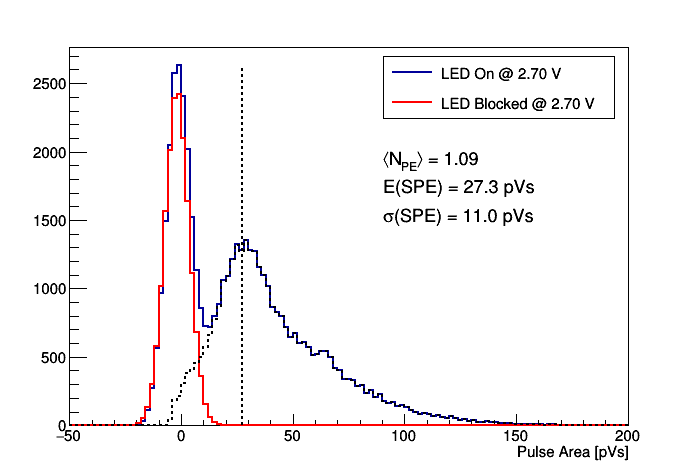
\includegraphics[width=0.49\textwidth]{figures/speAreaR8781250}}~
    \subfloat[][$1350\unit{V}$]{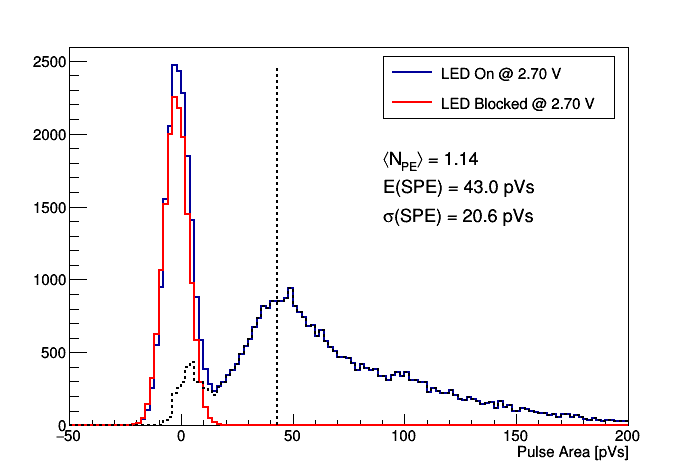
\includegraphics[width=0.49\textwidth]{figures/speAreaR8781350}}\\
    \subfloat[][$1450\unit{V}$]{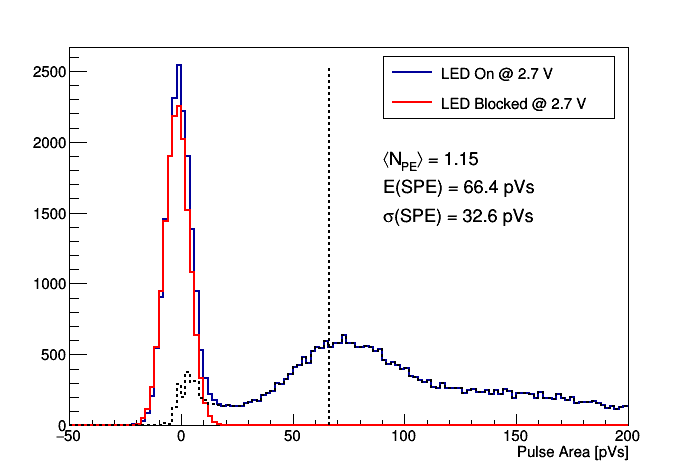
\includegraphics[width=0.49\textwidth]{figures/speAreaR8781450}}
    \caption{\label{fig:r878calib} The pulse area distributions used to calibrate the SPE area
    of an R878 PMT for a range of HV values.}
\end{figure}

\begin{figure}[ht!]
    \centering
    \subfloat[][$1250\unit{V}$]{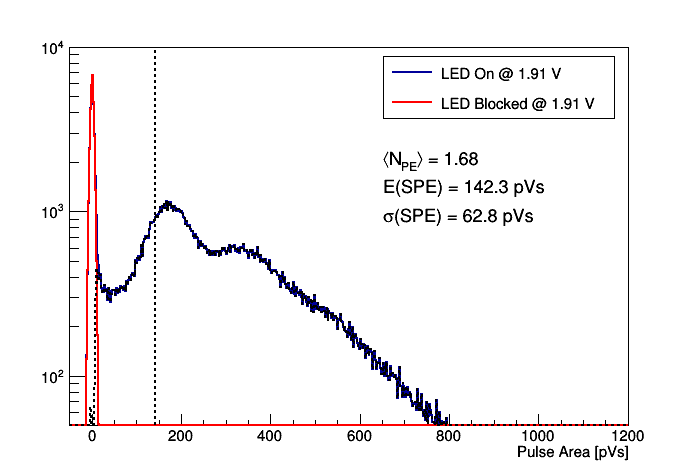
\includegraphics[width=0.49\textwidth]{figures/speAreaR77251400}}~
    \subfloat[][$1350\unit{V}$]{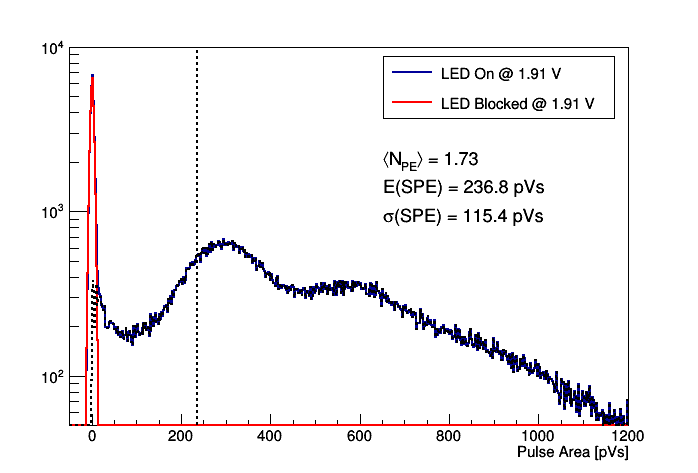
\includegraphics[width=0.49\textwidth]{figures/speAreaR77251500}}\\
    \subfloat[][$1450\unit{V}$]{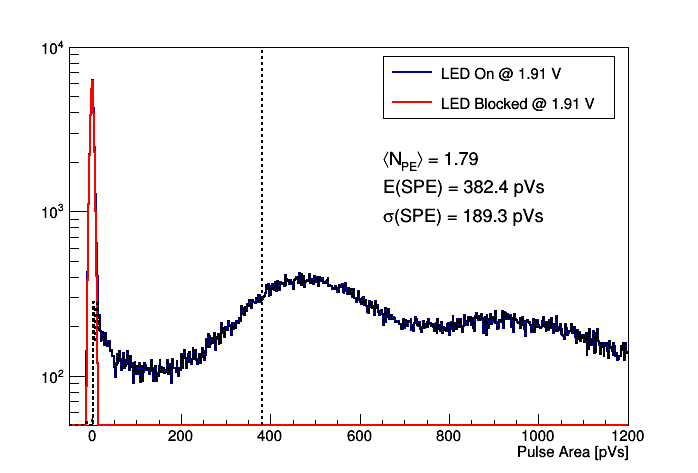
\includegraphics[width=0.49\textwidth]{figures/speAreaR77251600}}
    \caption{\label{fig:r7725calib} The pulse area distributions used to calibrate the SPE area
    of an R7725 PMT for a range of HV values.}
\end{figure}

\begin{figure}[ht!]
    \centering
    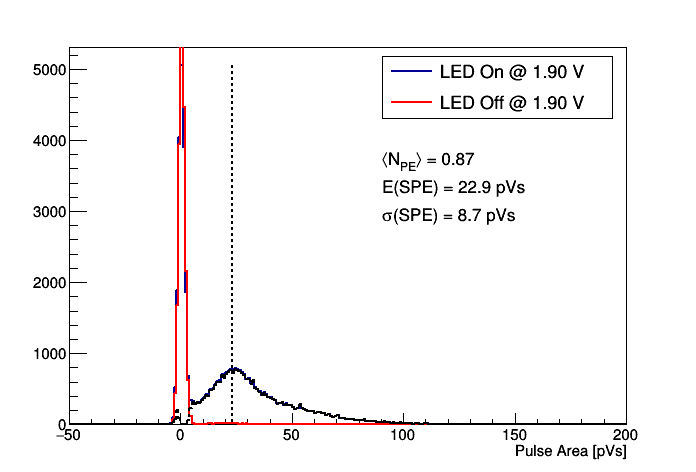
\includegraphics[width=0.49\textwidth]{figures/speAreaEt1700}
    \caption{\label{fig:etcalib} The pulse area distributions used to calibrate the SPE area
    of an ET PMT for a HV of 1700\unit{V}.}
\end{figure}

\subsection{Afterpulse characterisation}

Afterpulses are caused by the production of positive ions in residual
gases in the PMT tube. These ions return to the photocathode and produce
a significant number of photoelectrons. The amplitude and time delay
depend on the mass and charge of the ion as well as the position of the 
production of the ion. The time delay typically ranges from several 
hundred nanoseconds to a few microseconds or more. In the later case
this can cause a correlated background in the detector if there are
overlapping afterpulses from a single correlated source (which would lie outside
of the trigger window).

The afterpulse behaviour was studied for the R878 and R7725 PMT 
considered in Section~\ref{sec:ledarea}. The time window was expanded to
a microsecond and the afterpulse spectrum measured by
averaging the waveforms after subtracting the time of the initial pulse.
The results are shown in Figure~\ref{fig:afterpulse} for the R878 and R7725 PMTs.
The R878 shows several peaks with the largest occuring at $\sim 400\unit{ns}$ while 
the R7725 has a single large peak at $\sim 500\unit{ns}$. Finally, the average waveform
for various HV values is shown in Figure~\ref{fig:afterpulseVsHV}. The peak
time is expected to follow an inverse square root HV dependance~\cite{MA201193} and,
while this requires further study, can be seen in Figure~\ref{fig:peakTimeDep}.

\begin{figure}[ht!]
    \centering
    \subfloat[][R878]{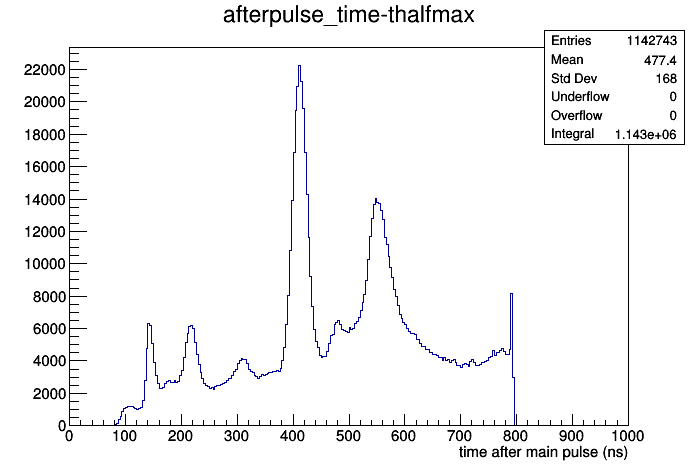
\includegraphics[width=0.49\textwidth]{figures/afterpulseLEDR878.png}}~
    \subfloat[][R7725]{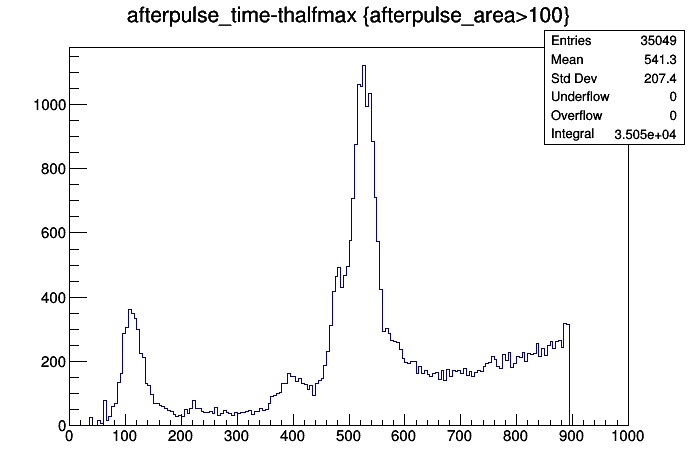
\includegraphics[width=0.49\textwidth]{figures/afterpulseLEDR7725.png}}
    \caption{\label{fig:afterpulse} The average waveform spectrum for two PMTs. The peaks correspond 
    to afterpulses.
    }
\end{figure}

\begin{figure}[ht!]
    \centering
    \subfloat[][\label{fig:afterpulseVsHV}]{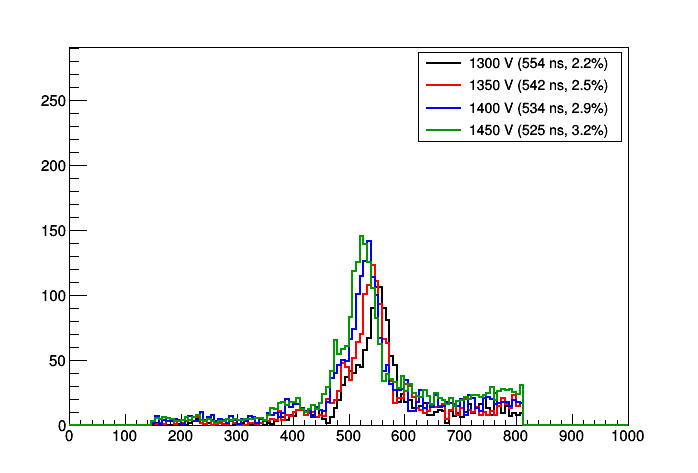
\includegraphics[width=0.49\textwidth]{figures/afterpulseLEDR7725VsHV.png}}~
    \subfloat[][\label{fig:peakTimeDep}]{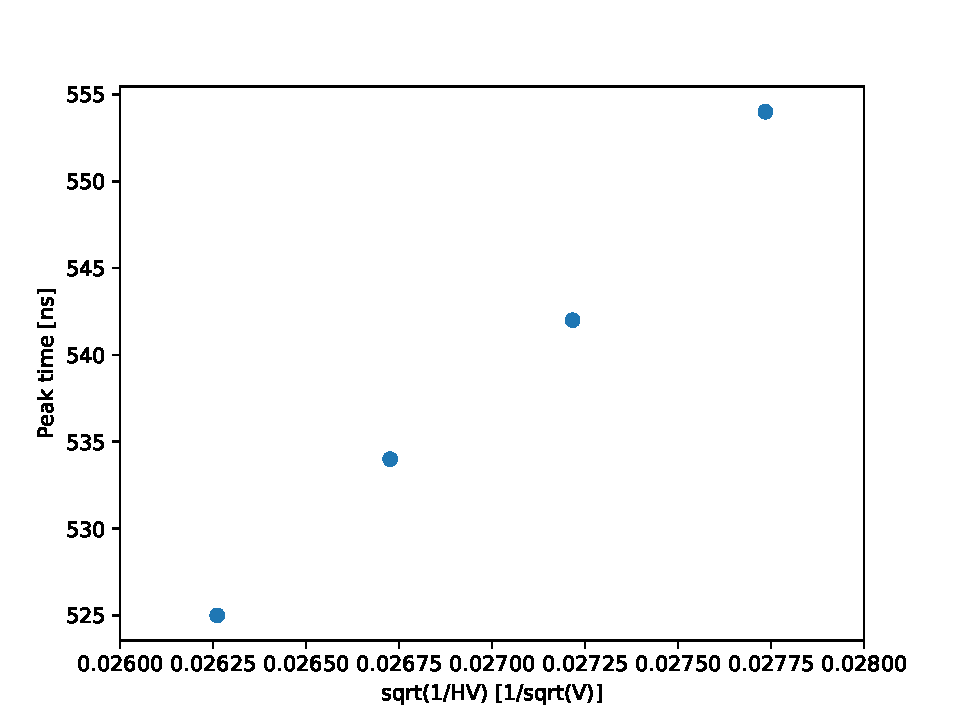
\includegraphics[width=0.49\textwidth]{figures/peakTimeDep}}
    \caption{(a) The average waveform spectrum for the R7725 PMT for
    several HV values. (b) The peak time follows an inverse square root dependence with the HV.}
\end{figure}

\subsection{SPE pulse shape and area spectrum}

The LED is finally used to measure the average SPE waveform and 
are spectrum. This is carried out for an R878 and R7725 PMT. 
The pulse shape is measured by averaging many individual 
pulses and the resultant templates are shown in Figure~\ref{fig:speTemplate}.
The average waveform for the R7725 is significantly narrower than for the R878.
The SPE area spectrum is measured by using a very low LED intensity to eliminate
contamination from 2 or more SPE events. The zero PE component is then subtracted following
the same procedure in~\ref{sec:ledarea} and the resultant SPE area distribution for the R7725 shown in 
Figure~\ref{fig:speareaspectrum}. There is an exponential tail from suboptimal trajectories at low
pulse areas and a Gaussian core around $\sim500\unit{ps}$. The contamination from 2 or more SPE events
is $\sim 3\%$.

\begin{figure}[ht!]
    \centering
    \subfloat[][R878]{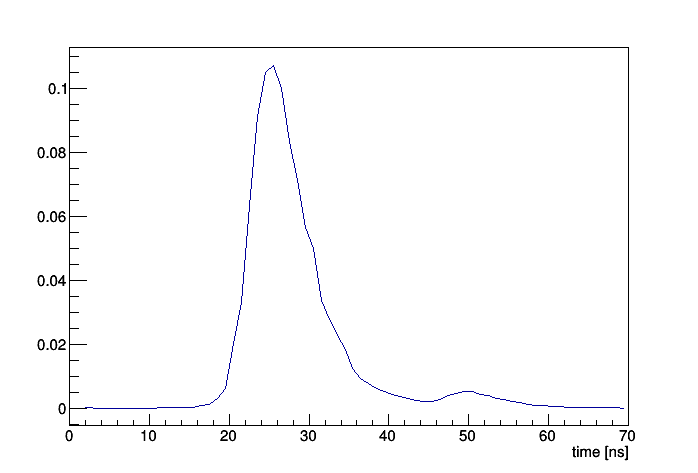
\includegraphics[width=0.49\textwidth]{figures/speTemplateLEDR878.png}}~
    \subfloat[][R7725]{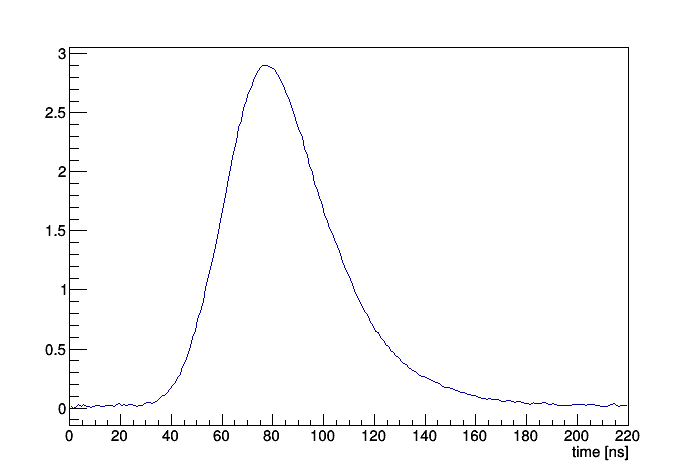
\includegraphics[width=0.49\textwidth]{figures/speTemplateLEDR7725.png}}
    \caption{\label{fig:speTemplate} The average waveform spectrum for the R7725 PMT for
    several HV values. The peak time follows an inverse square root de dependence pendance with the HV.}
\end{figure}

\begin{figure}[ht!]
    \centering
    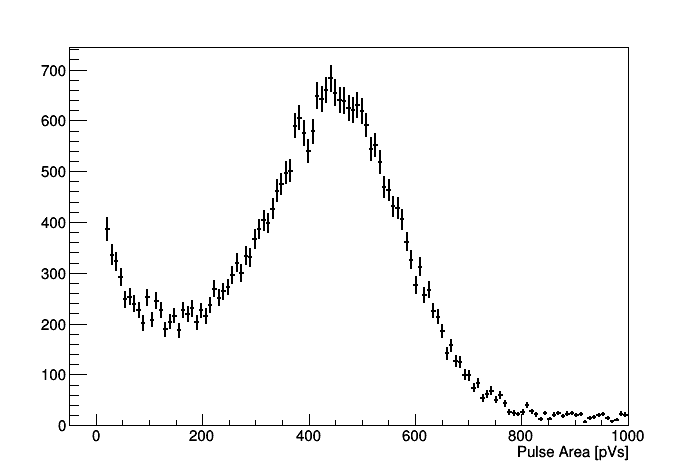
\includegraphics[width=0.49\textwidth]{figures/speAreaSpectrum}
    \caption{\label{fig:speareaspectrum} The measurement of the SPE area spectrum for an R7725 PMT.}
\end{figure}

\clearpage

\bibliographystyle{unsrt}
\bibliography{milliqanAnalysis}

\end{document}
